\documentclass[10pt]{article}
\usepackage[a4paper]{geometry}
\setlength\parindent{0pt}
\usepackage{enumitem}
\usepackage{comment}
\usepackage{float}
\setlength{\footnotesep}{0.4cm}
\usepackage{multicol}
\usepackage{blindtext}
\usepackage{changepage} 
\usepackage{lipsum} 
\setlength{\skip\footins}{0.5cm}
\renewcommand{\footnoterule}{%
  \kern -3pt
  \hrule width \textwidth height 0.1pt
  \kern 2.6pt
}
\usepackage{tabularx}
\usepackage {amsmath}
\usepackage{authblk}

\usepackage{hyperref}
\hypersetup{
	colorlinks=true,
    linkcolor=blue,
    filecolor=magenta,      
    urlcolor=cyan,
    pdftitle={Viral-Technical Whitepaper}
}

\usepackage{color}
\definecolor{light}{rgb}{0.5, 0.5, 0.5}
\def\light#1{{\color{light}#1}}


\usepackage{listings}
% Copyright 2017 Sergei Tikhomirov, MIT License
% https://github.com/s-tikhomirov/solidity-latex-highlighting/

\usepackage{listings, xcolor}

\definecolor{verylightgray}{rgb}{.97,.97,.97}

\lstdefinelanguage{Solidity}{
	keywords=[1]{anonymous, assembly, assert, balance, break, call, callcode, case, catch, class, constant, continue, constructor, contract, debugger, default, delegatecall, delete, do, else, emit, event, experimental, export, external, false, finally, for, function, gas, if, implements, import, in, indexed, instanceof, interface, internal, is, length, library, log0, log1, log2, log3, log4, memory, modifier, new, payable, pragma, private, protected, public, pure, push, require, return, returns, revert, selfdestruct, send, solidity, storage, struct, suicide, super, switch, then, this, throw, transfer, true, try, typeof, using, value, view, while, with, addmod, ecrecover, keccak256, mulmod, ripemd160, sha256, sha3}, % generic keywords including crypto operations
	keywordstyle=[1]\color{blue}\bfseries,
	keywords=[2]{address, bool, byte, bytes, bytes1, bytes2, bytes3, bytes4, bytes5, bytes6, bytes7, bytes8, bytes9, bytes10, bytes11, bytes12, bytes13, bytes14, bytes15, bytes16, bytes17, bytes18, bytes19, bytes20, bytes21, bytes22, bytes23, bytes24, bytes25, bytes26, bytes27, bytes28, bytes29, bytes30, bytes31, bytes32, enum, int, int8, int16, int24, int32, int40, int48, int56, int64, int72, int80, int88, int96, int104, int112, int120, int128, int136, int144, int152, int160, int168, int176, int184, int192, int200, int208, int216, int224, int232, int240, int248, int256, mapping, string, uint, uint8, uint16, uint24, uint32, uint40, uint48, uint56, uint64, uint72, uint80, uint88, uint96, uint104, uint112, uint120, uint128, uint136, uint144, uint152, uint160, uint168, uint176, uint184, uint192, uint200, uint208, uint216, uint224, uint232, uint240, uint248, uint256, var, void, ether, finney, szabo, wei, days, hours, minutes, seconds, weeks, years},	% types; money and time units
	keywordstyle=[2]\color{teal}\bfseries,
	keywords=[3]{block, blockhash, coinbase, difficulty, gaslimit, number, timestamp, msg, data, gas, sender, sig, value, now, tx, gasprice, origin},	% environment variables
	keywordstyle=[3]\color{violet}\bfseries,
	identifierstyle=\color{black},
	sensitive=false,
	comment=[l]{//},
	morecomment=[s]{/*}{*/},
	commentstyle=\color{gray}\ttfamily,
	stringstyle=\color{red}\ttfamily,
	morestring=[b]',
	morestring=[b]"
}

\lstset{
	language=Solidity,
	backgroundcolor=\color{verylightgray},
	extendedchars=true,
	basicstyle=\footnotesize\ttfamily,
	showstringspaces=false,
	showspaces=false,
	numbers=left,
	numberstyle=\footnotesize,
	numbersep=9pt,
	tabsize=2,
	breaklines=true,
	showtabs=false,
	captionpos=b
}

\usepackage{tikz}
\usetikzlibrary{shapes.geometric , arrows}
\usetikzlibrary{mindmap,trees}
\usepackage{adjustbox}
\usepackage[edges]{forest}
\usetikzlibrary{arrows.meta}

%tikzlibrary

\tikzstyle{st} = [rectangle, rounded corners, minimum width=3cm, minimum height=0.6cm, text width=3cm, text centered, draw=black, fill=red!15]
\tikzstyle{io} = [trapezium, trapezium left angle=70, trapezium right angle=110, minimum width=2cm,text width=3cm,  minimum height=0.6cm, text centered, draw=black, fill=blue!15]
\tikzstyle{pro} = [rectangle, minimum width=3cm, minimum height=0.6cm,  text centered,text width=3cm, draw=black, fill=orange!15]
\tikzstyle{dec} = [diamond, minimum width=3cm,  minimum height=0.6cm, text centered, draw=black,text width=3cm, fill=green!15]
\tikzstyle{arrow} = [thick,->,>=stealth]
\def\checkmark{\tikz\fill[scale=0.4](0,.35) -- (.25,0) -- (1,.7) -- (.25,.15) -- cycle;} 

%tikzlibrary

\usepackage{multirow}
\usepackage{tfrupee}
\usepackage{fancyhdr}
\pagestyle{fancy}
\fancyfoot[C]{
\begin{center}

\includegraphics[width=0.4cm]{logo}\\
\vspace{1mm}
\thepage\\
\vspace{0.3mm}
\footnotesize{\light{viralfoundation.org}}
\end{center}
}







\newlength{\Lnote}
\newcommand{\notte}[1]
     {\addtolength{\leftmargini}{1em}
        \settowidth{\Lnote}{\textbf{Note:~}}
        \begin{quote}
            \rule{\dimexpr\textwidth-2\leftmargini}{1pt}\\
                        \mbox{}\hspace{-\Lnote}\textbf{Note:~}%
                                            #1\\[-0.5ex] 
            \rule{\dimexpr\textwidth-2\leftmargini}{1pt}
        \end{quote}
        \addtolength{\leftmargini}{-4em}}
\graphicspath{ {./assets/images/} }

\title{\textbf{Viral - Next Gen Social Communication \& User Experience}}
\date{15 January 2022}
\author{Joby Reuben}



\begin{document}


\maketitle

\begin{abstract}
\lipsum[1]\lipsum[1]
\end{abstract}

\vspace{5mm} %5mm vertical space

\textbf{Contributors}
\begin{enumerate}
\item{Ajay Joshua}
\item{Naveen Jose}
\item {Samarth Kulkarni}
\end{enumerate}

\newpage
   \tableofcontents\pagebreak 
   
\section{User Problems and Basic Solutions}
This is a Sample Problems of the Viral Project.

\section{Fad of Decentralized Social Media Apps}

\section{Vision Statement}
To bring blockchain and crypto adoption to the masses we would got to bridge social communication with defi and tokenised economy. The Viral Network of Applications standards are designed in such a way that our vision to bring an proficient, user-friendly mobile application will combine several divisions of decentralized protocols that can lead to an ultimate tool for crypto acknowledgement. The divisions which we are focussing to rebuild is listed\\
\\
\textbf{\large Social Media}
\begin{enumerate}
\item To create a Real-world Decentralised Social Media
\item To construct an Autonomous self-evolving platform
\item To construct an Interactive Next-Gen Social Media
To form a clean people-owned platform appropriate for all age groups
\end{enumerate}
\textbf{\large Crypto Adoption}
\begin{enumerate}
\item To provide people to hop into crypto from fiat effortlessly and securely
\item To give access to use cryptocurrencies to internet people without investing
\item To bring all major crypto for individuals to adapt rapidly using a single wallet
\end{enumerate}
\textbf{\large NFT and Metaverse}
\begin{enumerate}
\item To democratize NFTs to Masses
\item To kickstart Metaverse adoption
\end{enumerate}
\textbf{\large Blockchain}
\begin{enumerate}
\item To supply the utmost speed of transactions through On-Chain and Off-Chain solutions
\item To Develop a feeless, fast, Zero Inflation, Deflationary, smart contract chain
\end{enumerate}

\newpage
\section{Unified Mobile Application - An Intro to Viral}


External Links : \hyperlink{https://sample.com}{App-Brouchure},\ \hyperlink{https://sample.com}{Intro-Video},\ \hyperlink{https://sample.com}{Light-Paper}\\


Viral is a Next-Gen Social Media platform bridging interactive media, NFTs, and blockchain technologies\textsc{\char13} underlying applications into an every-day user-based mobile app. Viral bridges Social Media with Blockchain, Wallets, Exchanges and NFT Markeplaces to bring the ultimate one-app for the common masses to adopt into the tokenised economy.\\

Every media shared on viral is an unique NFT where it can be utilized to create limitless achievable outcomes across the platform. Users can share ultra-short to short videos, thoughts through text, sell NFTs and additionally make communication between one-on-one, private groups and, open channels with total genuine privacy. App users will be benefitted from zero ads, cryptographic encryption, censorship-resistant and, also get to use various cryptocurrencies throughout the platform. Every user is an active contributor to the platform by which they receive rewards (payment) in Viral Coin for effectively utilizing the Viral Application and it\textsc{\char13}s child platforms.\\

\section{Viral Platform Architecture}

External Links : \hyperlink{https://sample.com}{ELI5-Explainer Video}\\

\begin{center}
\begin{adjustbox}{width=12cm}
    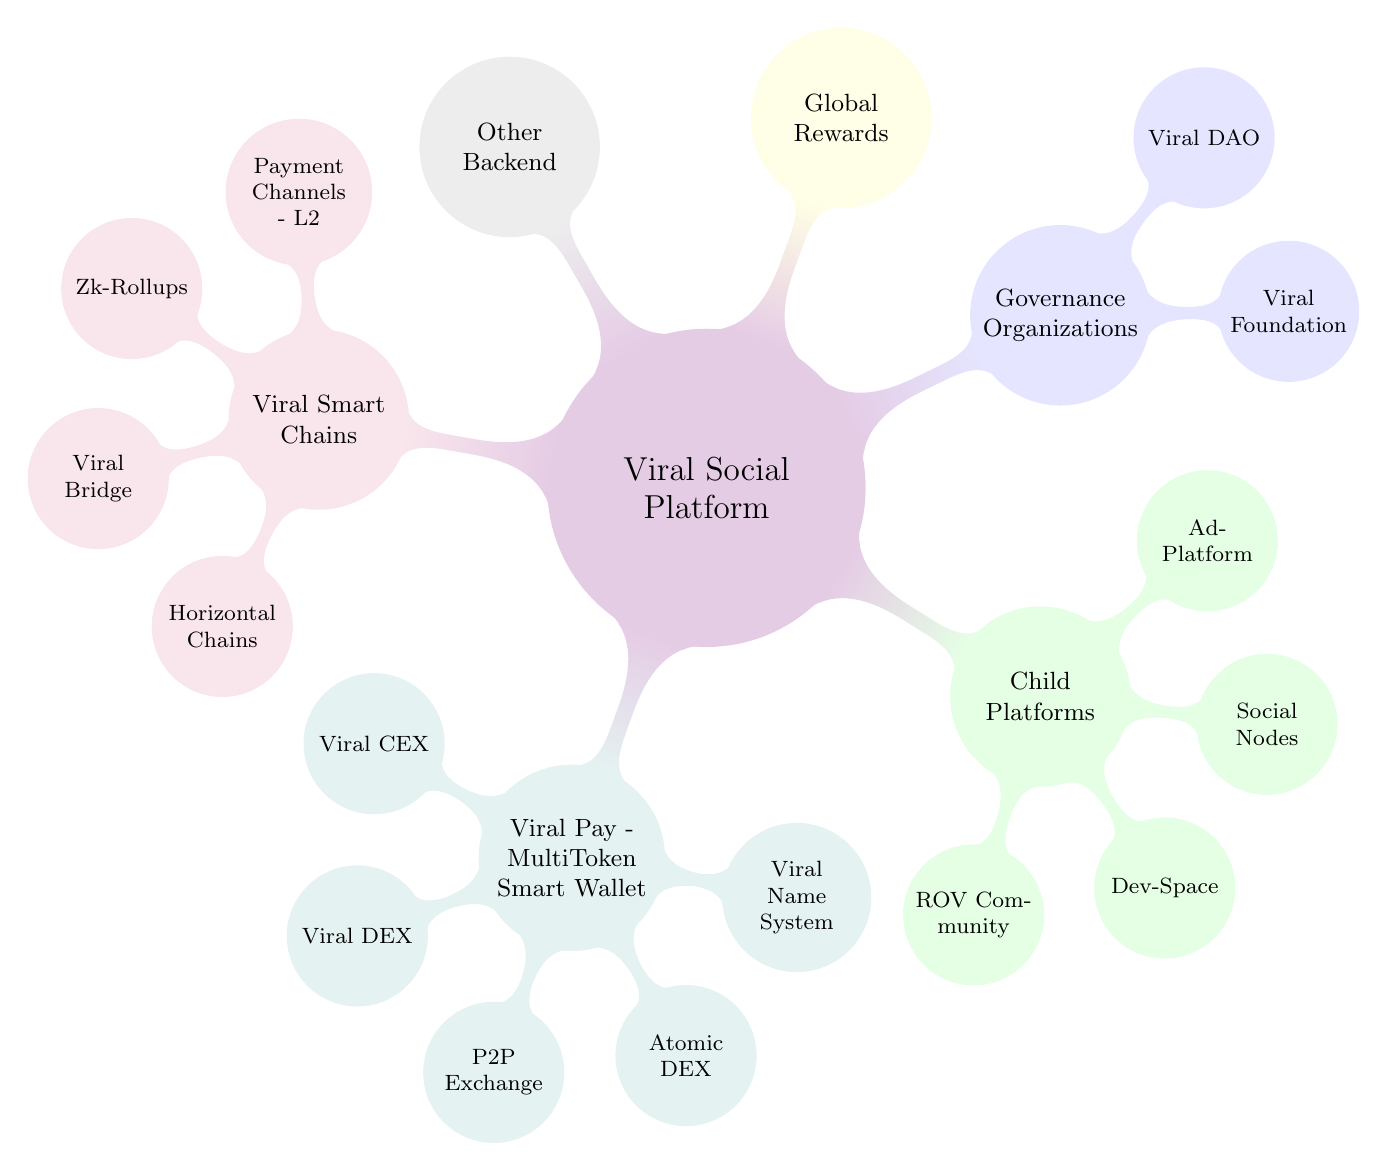
\begin{tikzpicture}
      [mindmap,
      grow cyclic,
      every node/.style=concept,
      concept color=violet!20,
      level 1/.append style={sibling angle=360/6},
      level 2/.append style={sibling angle=50},
      ]
      \node [root concept] {Viral Social Platform}
        child [concept color=purple!10, rotate=-40]{
          node    {Viral Smart Chains}
          child { node    {Payment Channels - L2} }
          child { node    {Zk-Rollups} }
          child { node    {Viral Bridge}}
          child { node    {Horizontal Chains} }
        }
        child [concept color=teal!10, rotate=-20]{
          node     {Viral Pay - MultiToken Smart Wallet}
          child { node    {Viral CEX} }
          child { node    {Viral DEX} }
          child { node    {P2P Exchange} }
          child { node    {Atomic DEX} }
          child { node    {Viral Name System} }
        }
        child [concept color=green!10, rotate=-2]{
          node  {Child Platforms}
          child { node {ROV Community} }
          child { node {Dev-Space} }
          child { node {Social Nodes} }
          child { node {Ad-Platform} }
        }
        child [concept color=blue!10, rotate=-4]{
          node  {Governance Organizations}
          child { node {Viral Foundation} }
          child { node {Viral DAO} }
        }
        child [concept color=yellow!10, rotate=-20]{
          node   {Global Rewards}%[clockwise from=45, level distance=8cm]
        }
        child [concept color=black!7, rotate=-30] {
          node {Other Backend}}
        ;  
        
        \end{tikzpicture}
\end{adjustbox}
\end{center}

\begin{enumerate}

\item \textbf{Viral App}: Decentralized Social Media Platform bridging Blockchain applications for limitless possibilities.

\item \textbf{Viral Smart Chains}: Horizontally Scalable EVM Smart Chain on Top of IOTA\textsc{\char13}s Tangle.

\begin{enumerate}

	\item \textbf{Payment Channels (L2)}: State Channels to move value off-chain for lightning fast micro-transactions.

	\item \textbf{Zk-Rollups (L2)}: Batching Multiple Off-chain NFT Standard Tokens (ERC721) to On-Chain,
	\item \textbf{Viral Bridge}: Interopability of various major cryotocurrencies by wrapping tokens decentralized such as Bitcoin, Ethereum,etc into Viral Smart Chains.
	\item \textbf{Horizontal Chains}: Additional of New Chains anchored to IOTA Tangle that communicates between multiple Viral Smart Chains for unlimited scaling

\end{enumerate}

\item \textbf{Viral Pay - Multi-Token Smart Wallet}: Viral\textsc{\char13}s App\textsc{\char13}s built in Non-Custodial Viral Smart Chain compatible hot wallet that allows user to send and hold tokens, mint NFTs and receive rewards.

\begin{enumerate}

\item \textbf{Viral CEX-Centralized Exchange}: Trustless Non-Custodial Exchange for Fiat-Crypto trading
\item \textbf{Viral DEX-Decentralized Exchange}: Automated Market Making Protocol for exchanging Viral tokens
\item \textbf{P2P Exchange}: Trustsless anonymous exchange leveraging Peer-to-Peer protocol
\item \textbf{Viral Name System}: Decentralized blockchain based username protocol for transfers instead of cryptographic public address.

\end{enumerate}

\item \textbf{Child Platforms}: Independent platforms anchored to the viral network for effective improvement of protocols

\begin{enumerate}

\item \textbf{Dev-Space}: Application for Developers to decide on reward allocation for improving Viral-Beta
\item \textbf{ROV Community}: Curator Platform to vote and remove reported content on Viral-Alpha
\item \textbf{Ad Platform}: Decentralized Ad platform connecting Influencers,businesses and users for trustless engagement-proof ads.

\end{enumerate}

\item \textbf{Global Rewards}: To incentivize all users, miners, developers using smart contracts for their content, validation of transactions, and continuous development through unbiased pointing strategy that offers more rewards to bigger contributors.


\item \textbf{Other Backend}: For contingencies which will be later decentralized in the further phases of the development roadmap

	

\end{enumerate}

	\subsection{Development Tech Stack}

	\begin{enumerate}

	\item \hyperlink{https://ipfs.io}{IPFS}: IPFS stands for Interplanetary File System is a peer-to-peer distributed file system that is used for maintaining and distributing files across our Viral IPFS Private network.

	\item \hyperlink{https://gun.eco/}{GunDB}: GunDB is a fully decentralized graph database to store information from user to user meaning that your changes are not affected by any centralized server.

	\item \hyperlink{https://webrtc.org/}{WebRTC}: WebRTC stands for Web Real-Time Communication, an open-source project built primarily for peer-to-peer real-time connections.

	\item \hyperlink{https://www.javascript.com/}{Javascript}: JavaScript is a text-based programming language used both on the client-side and server-side that allows you to make web pages interactive.

	\item \hyperlink{https://nodejs.org/}{NodeJS}: Node.js is an open-source, cross-platform, back-end JavaScript runtime environment that runs on the V8 engine and executes JavaScript code outside a web browser.

	\item \hyperlink{https://reactjs.org/}{ReactJS}: React is a free and open-source front-end JavaScript library for building user interfaces based on UI components.

	\item \hyperlink{https://docs.soliditylang.org/}{Solidity}:Solidity is an object-oriented, high-level language for implementing smart contracts, mostly used for executing code in Ethereum Virtual Machine

	\item \hyperlink{https://wiki.iota.org/smart-contracts/overview}{IOTA Smart Contract Protocol}: The IOTA ecosystem allows to spin up a smart contract blockchain and anchor it to the IOTA tangle
	
	\end{enumerate}


\section{How Whitepaper Structured}
For an efficient understanding, we have seperated the Viral Architecture/Ecosystem\textsc{\char13}s major sectors.\\

\begin{itemize}[leftmargin=+0.2in]
\item Social Media and User Experience (Page 1-10)
\item Blockchain, Token Ecosystem (Page 10-15)
\item Viral Pay - Multi-Token Smart Wallet (Page 15-20)
\item Child Platforms (Page 20-25)
\item Revenue and Incentives (Page 25-30)
\item Viral DAO  and Governance
\end{itemize}

\section{Social media and User Experience}
Viral is a multi-media sharing decentralized social network that brings meta-experience with friends, family and other people to communicate, share posts and send messages across the globe with absolute privacy. Viral sets Non-Fungible-Tokens (NFT) as a standard for every post that shared in the network which intends to bring interactive social experience and utility use cases of blockchain environment.\\

\notte{To bring NFT as a standard for a social media post doesn\textsc{\char13}t essentially implies it ought to be sold for tokens, rather it conveys that each post in Viral is a unique piece of data in the blockchain that gives the power of ownership of the user which if needed can be opted to transfer in exchange for tokens inside the Viral Platform.\texttt{notte}.}

\subsection{Types of Post}
\hyperlink{https://sample.com}{ELI5 Explanatory Video - Viral NFTs}\\

Please read \hyperlink{App Brouchure}{https://sampel.com/} to have a visual experience of the Viral Social Network\\

\textit{Image for all Post Types in a Visualized Manner}

\textbf{Shots}

Shots are \textbf{10 sec motion pictures} with added loop transitions to bring life to photos. Pictures can be shared as shots, an exciting looped motion picture.\\

People can share their
\begin{enumerate}[leftmargin=+0.2in]
\item Personal Sneak-Peek, Moments and Events
\item Exclusive Photoshoots, commercials, to your fans
\item Turn photos into lively shots by adding shot animations through Viral
\end{enumerate}

\textbf{Thoughts}\\
Thoughts are \textbf{text-based sharing} for micro-blogging. Attach photos, long/short videos, documents, etc. There is no limit on words or media. People can share other users thoughts to their followers using re-Thought feature.\\


\textbf{Drops}\\

Drops are \textbf{20 second disappearing stories} shared to followers which auto-disappears once seen. It features AR filters, texts, shot elements, links, music, transitions and, much more. Every Drops will be purged in 30 days\\

\notte{Drops will not be minted as unique NFT due to it\textsc{\char13}s nature of disappearing media\texttt{notte}.}

\textbf{Interactive Videos}\\

IVs are short 30sec full-screen\textbf{narration based videos}. It is based on\textbf{gamification of videos} to interact within the videos.\\


\textbf{NFT Utilities}\\

Minting (Creating) an NFT in Viral is\textbf{as easy as creating a social media post}. Viral provides multiple NFT utilities for users to mint, buy, sell with an easy user experience.Viral will take a\textbf{1.5\% commission} selling NFTs which will be reverted to the reward pool\\


\textbf{Tunes}\\
Artists can\textbf{sell their music albums}, singles as NFT for the fans/people to buy and own it\\


\textbf{Sketch}\\
\textbf{Digital arts}, paintings, sketches can be sold through NFTs\\

\textbf{Originals}\\
\textbf{Physical assets} can be sold through Viral\textsc{\char13}s Original NFTs where people can buy and flex\\

\textbf{Tickets}\\
\textbf{Exclusive passes} for events, ownership of clubs, a digital ticket for everything can be sold as NFT. See Listing \ref{single-asset}\\

\textbf{Filters}\\
Filters can be sold, and owned by user\textsc{\char13}s thereby get rewards for it\\

Please read \hyperlink{App Brouchure}{https://sampel.com/} to have a visual experience of the Viral Social Network

\newpage

\begin{lstlisting}[language=Solidity, caption={NFT Snippet for Enable/Disable Open Sale}, numbers=none]

pragma solidity ^0.8.10;

contract HelloWorld {

    string public greet = "Hello World!";
    
}
\end{lstlisting}

\begin{lstlisting}[language=Solidity, caption={NFT Snippet To Sell Multiple Copies}, numbers=none]

pragma solidity ^0.8.10;

contract HelloWorld {

    string public greet = "Hello World!";
    
}
\end{lstlisting}

\begin{lstlisting}[language=Solidity,label={single-asset}, caption={NFT Snippet to sell single asset}, numbers=none]

pragma solidity ^0.8.10;

contract HelloWorld {

    string public greet = "Hello World!";
    
}
\end{lstlisting}

\begin{lstlisting}[language=Solidity, caption={NFT Snippet to provide extra information such as Name, Address, Mobile Number, before transferring coins with end to end encryption between seller}, numbers=none]

pragma solidity ^0.8.10;

contract HelloWorld {

    string public greet = "Hello World!";
    
}
\end{lstlisting}

\begin{lstlisting}[language=Solidity, caption={NFT Snippet to distribute shares Just like company share where if 100 NFTs is sold, the person who holds 50 NFT will hold 50\% of the company}, numbers=none]

pragma solidity ^0.8.10;

contract HelloWorld {

    string public greet = "Hello World!";
    
}
\end{lstlisting}

\pagebreak

\subsection{Avatars}

Personalized Avatars are generated free for every viral user using a selfie. Users can edit their avatar skin, outfit, hair, etc. These avatars will be shown in their public profile where other users can see them 3D View.\\

\textit{Image}\\

These avatars are brought into Viral to integrate metaverse and to provide an \textbf{interactive experience}\\

\hyperlink{https://sample.com}{Avatar Demo-Video}\\

\begin{lstlisting}[language=Solidity]

// ReadyPlayerMe Integration Examples

1. ReadyPlayerMe WebView- How creating Avatars work using Partner API
2. Downloading Asset- GLB File using Event Listener
3. Mapping skeletons and face
4. Animating and storing the file as a 3D Viewer File inside the application using IPFS Public/Clusters
5. How Animations will work

\end{lstlisting}

\subsubsection{Meta-Chat}

Meta-Chat is a feature to \textbf{show your facial reactions} in real-time when you chat with your friend. Viral captures your face reactions and transfer it to your avatar which the mutual friend can see on \textbf{top of his/her chat page}.

\textit{Image}\\

This gives you a \textbf{virtual experience} of videocalls through avatars and text chat.

\hyperlink{https://sample.com}{Meta-Chat Demo}\\

\textbf{SDKs and APIs Used} : List the APIs\\

\textit{Formula\\
Flowcharts}

\subsubsection{Live and Rooms}

Decentralized \textbf{Live Video Events and Audio Rooms using Avatars} (or) Normal Cams. Celebrities can host live events with their fans using their avatars\\

\textit{Image}\\
\hyperlink{https://sample.com}{Live-Events Demo}\\

\textbf{SDKs and APIs Used} : List the APIs\\

\textit{Formula\\
Flowcharts}

\subsection{Engagements}

\textbf{Like, Comment, Share, Tip}\\

Users can like, comment, share, reThought, and also tip Tokens to their favorite posts and influencers. The number of likes will influence the recommendations list of other users.\\

Additionally a hidden engagement dislike will be added to every post but won\textsc{\char13}t be visible to the users/nor owners, which is exclusively utilized for interest-based algorithm to filter out disliked content\\

\textit{Algorithm/Mathematical formula for recommendation engine}\\

\textbf{Tip}\\

The tipping feature in Viral engagements tip/support user\textsc{\char13}s favourite influencers\textsc{\char13} contents. It works as a donation/reward where all the tips will be directly sent to the receivers wallet. Users can send tokens of their own choice to reward other users content on the platform.

Viral will charge commisions on Tips and deposits it to the reward pool. These commissions are calculated in such a way where the percentage varies depending on the end face value.\\

The tipping amount will be round of to tens and will leave the commision on both seperated amounts.\\

$Formula$\\

The Charges are\\


(Ending with 1,2)\$ tips     - 22\%      i.e., 11, 62, 761, 952\\
(Ending with 3,4,5)\$ tips   - 19\%      i.e., 23, 64, 765, 953\\
(Ending with 6,7,8,9)\$ tips - 17\%      i.e., 16, 48, 27,  79\\
(Ending with 0)\$ tips       - 12\%      i.e., 10, 60, 720, 1000\\


For example: If a user is tips worth 57\$ then the commissions charged will be:\\

For the first     50\$ - 12\%\\
And the remaining 7\$  - 17\%\\
\begin{figure}[H]
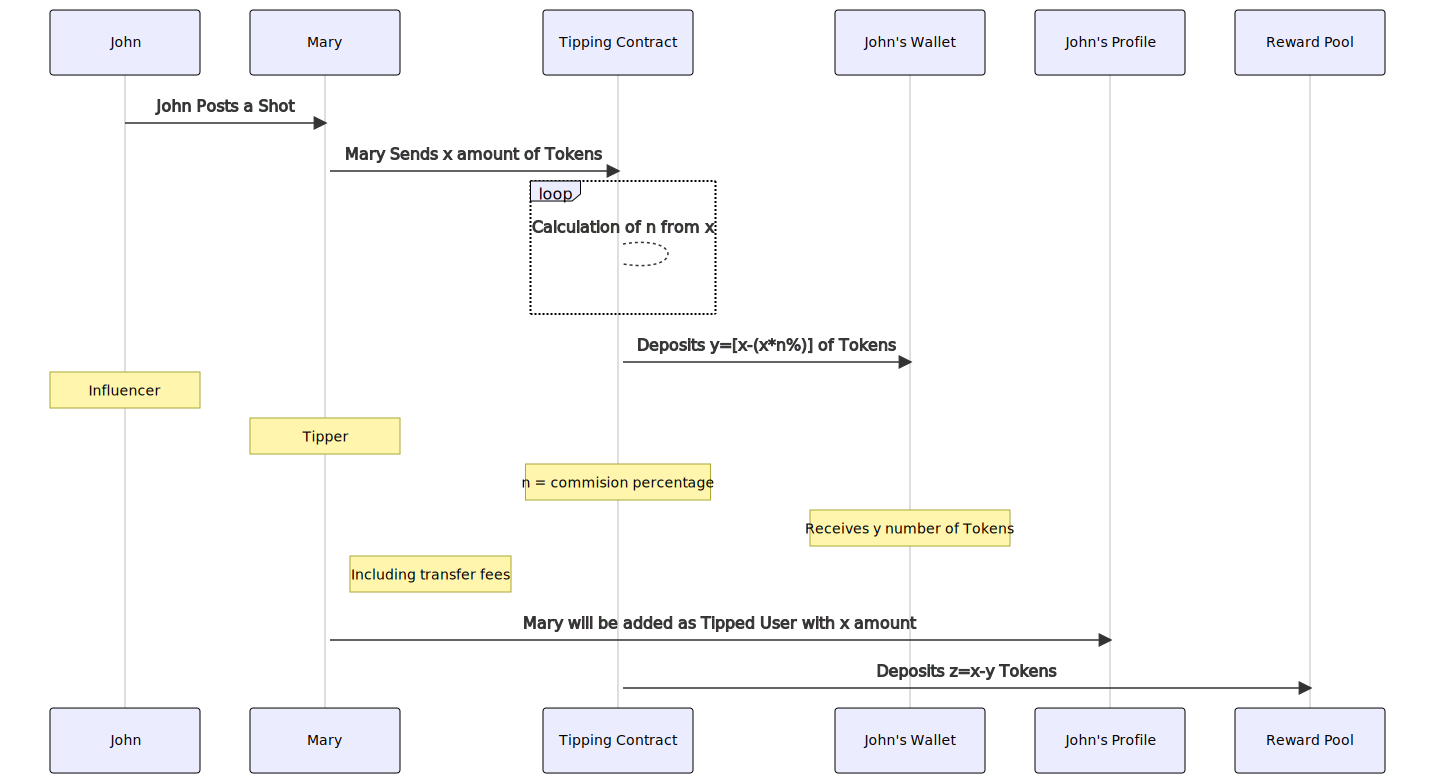
\includegraphics[width=\textwidth]{tips}\\
\caption{Tips Flowchart}
\end{figure}

\begin{comment}%mermaid

sequenceDiagram

    participant John
    participant Mary
    participant Tipping Contract
    participant John's Wallet
    participant John's Profile
    participant Reward Pool
    

    John->>+Mary:John Posts a Shot
    Mary->>+Tipping Contract:Mary Sends x amount of Tokens
    loop 
    Tipping Contract-->Tipping Contract:Calculation of n from x
    end
    Tipping Contract->>+John's Wallet:Deposits y=[x-(x*n%)] of Tokens
    Note over John: Influencer
    Note over Mary: Tipper
    Note over Tipping Contract: n = commision percentage
    Note over John's Wallet: Receives y number of Tokens
    Note right of Mary: Including transfer fees
    Mary->>+John's Profile: Mary will be added as Tipped User with x amount
    Tipping Contract->>+Reward Pool: Deposits z=x-y Tokens

\end{comment}


\begin{lstlisting}[language=Solidity, caption={Tipping Solidity Snippet}]

pragma solidity ^0.8.10;

contract HelloWorld {

    string public greet = "Hello World!";
    
}

\end{lstlisting}

\subsection{Other Features}

\subsubsection{Privacy Groups}

Privacy Groups is a unique feature in Viral to create unlimited friend\textsc{\char13}s groups list to ensure maximum privacy for users to post and share to particular groups of users i.e., Family, Friends, Close Friends, Besties, etc. This feature can empower complete privacy over viewers for certain posts.\\

\begin{figure}[H]
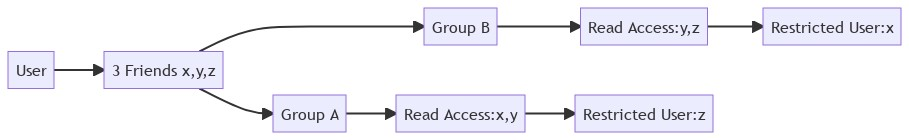
\includegraphics[width=\textwidth]{privacygroups}\\
\caption{Privacy Groups}
\end{figure}

\begin{comment}%mermaid
flowchart LR
    A[User]-->0
    0[3 Friends x,y,z]-->B[Group A]
    0--->C[Group B]
    B-->D[Read Access:x,y]
    C-->E[Read Access:y,z]
    D-->F[Restricted User:z]
    E-->G[Restricted User:x]
\end{comment}

\begin{lstlisting}[language=Solidity, caption={GunDB Privacy Group Snippet}]

pragma solidity ^0.8.10;

contract HelloWorld {

    string public greet = "Hello World!";
    
}
\end{lstlisting}

\subsubsection{Audio Emoji}

This is a short feature where all the emojis in Viral if touched will give a \textbf{short sound of the emoji}. This will be accessible on chats and comments section of a post.\\

\subsubsection{Interest Based Recommendation}

To make the viral platform more user-friendly interest-based recommendations are utilized. We have numerous ways to fetch interest from a user \textbf{without collecting data on a centralized server}, a few of them are\\

\begin{itemize}[leftmargin=+0.2in]
\item Like and Dislike
\item Hashtag Follows
\item Search-Based Interests
\item Based on Activity
\item Shares with other friends
\item Following interests
\item Based on Comments
\end{itemize}

All the user interests will be \textbf{stored locally} on the device to ensure \textbf{maximum security} and will be taken to show recommendations.\\

$Flow chart$

\subsection{User Security and Privacy}

At current world, privacy of user's in social media is being exploited by several centralized monopoly companies that run major social netwroking mobile applications that tracks user's data regarding their interests. These datas are being stored in a centralized database that is prone to attacks and breaches of private information. While targeted-manipulation plays a huge role in advertising industry, the collection of data is still prominent for almost 99\% social media business models except those run in donations. Viral focusses on maximum privacy of user's data by eliminating a central point of storage and heavily encrypts the media content circulating in the platform. It is possible to say Viral collects zero data of users and maintain a secure, trustable application in a generation where our mobiles are who we are.\\

This is classified into
\begin{enumerate}[leftmargin=+0.2in]
\item Media Storage
\item Chats or Private Messages
\item Interests of User
\item Chat backups
\end{enumerate}

\textbf{1. Media Storage}\\

All Media uploaded to Viral is End-to-end Encrypted where all the files are encrypted using Symmetric AES-256 Encryption Standard on the device and gets uploaded to Trustless IPFS Public Nodes and Trusted IPFS Cluster Nodes. Thus promising the security of media.\\

\textbf{Storing Files using IPFS}\\



\textbf{Encryption}\\

\begin{figure}[H]
\begin{center}
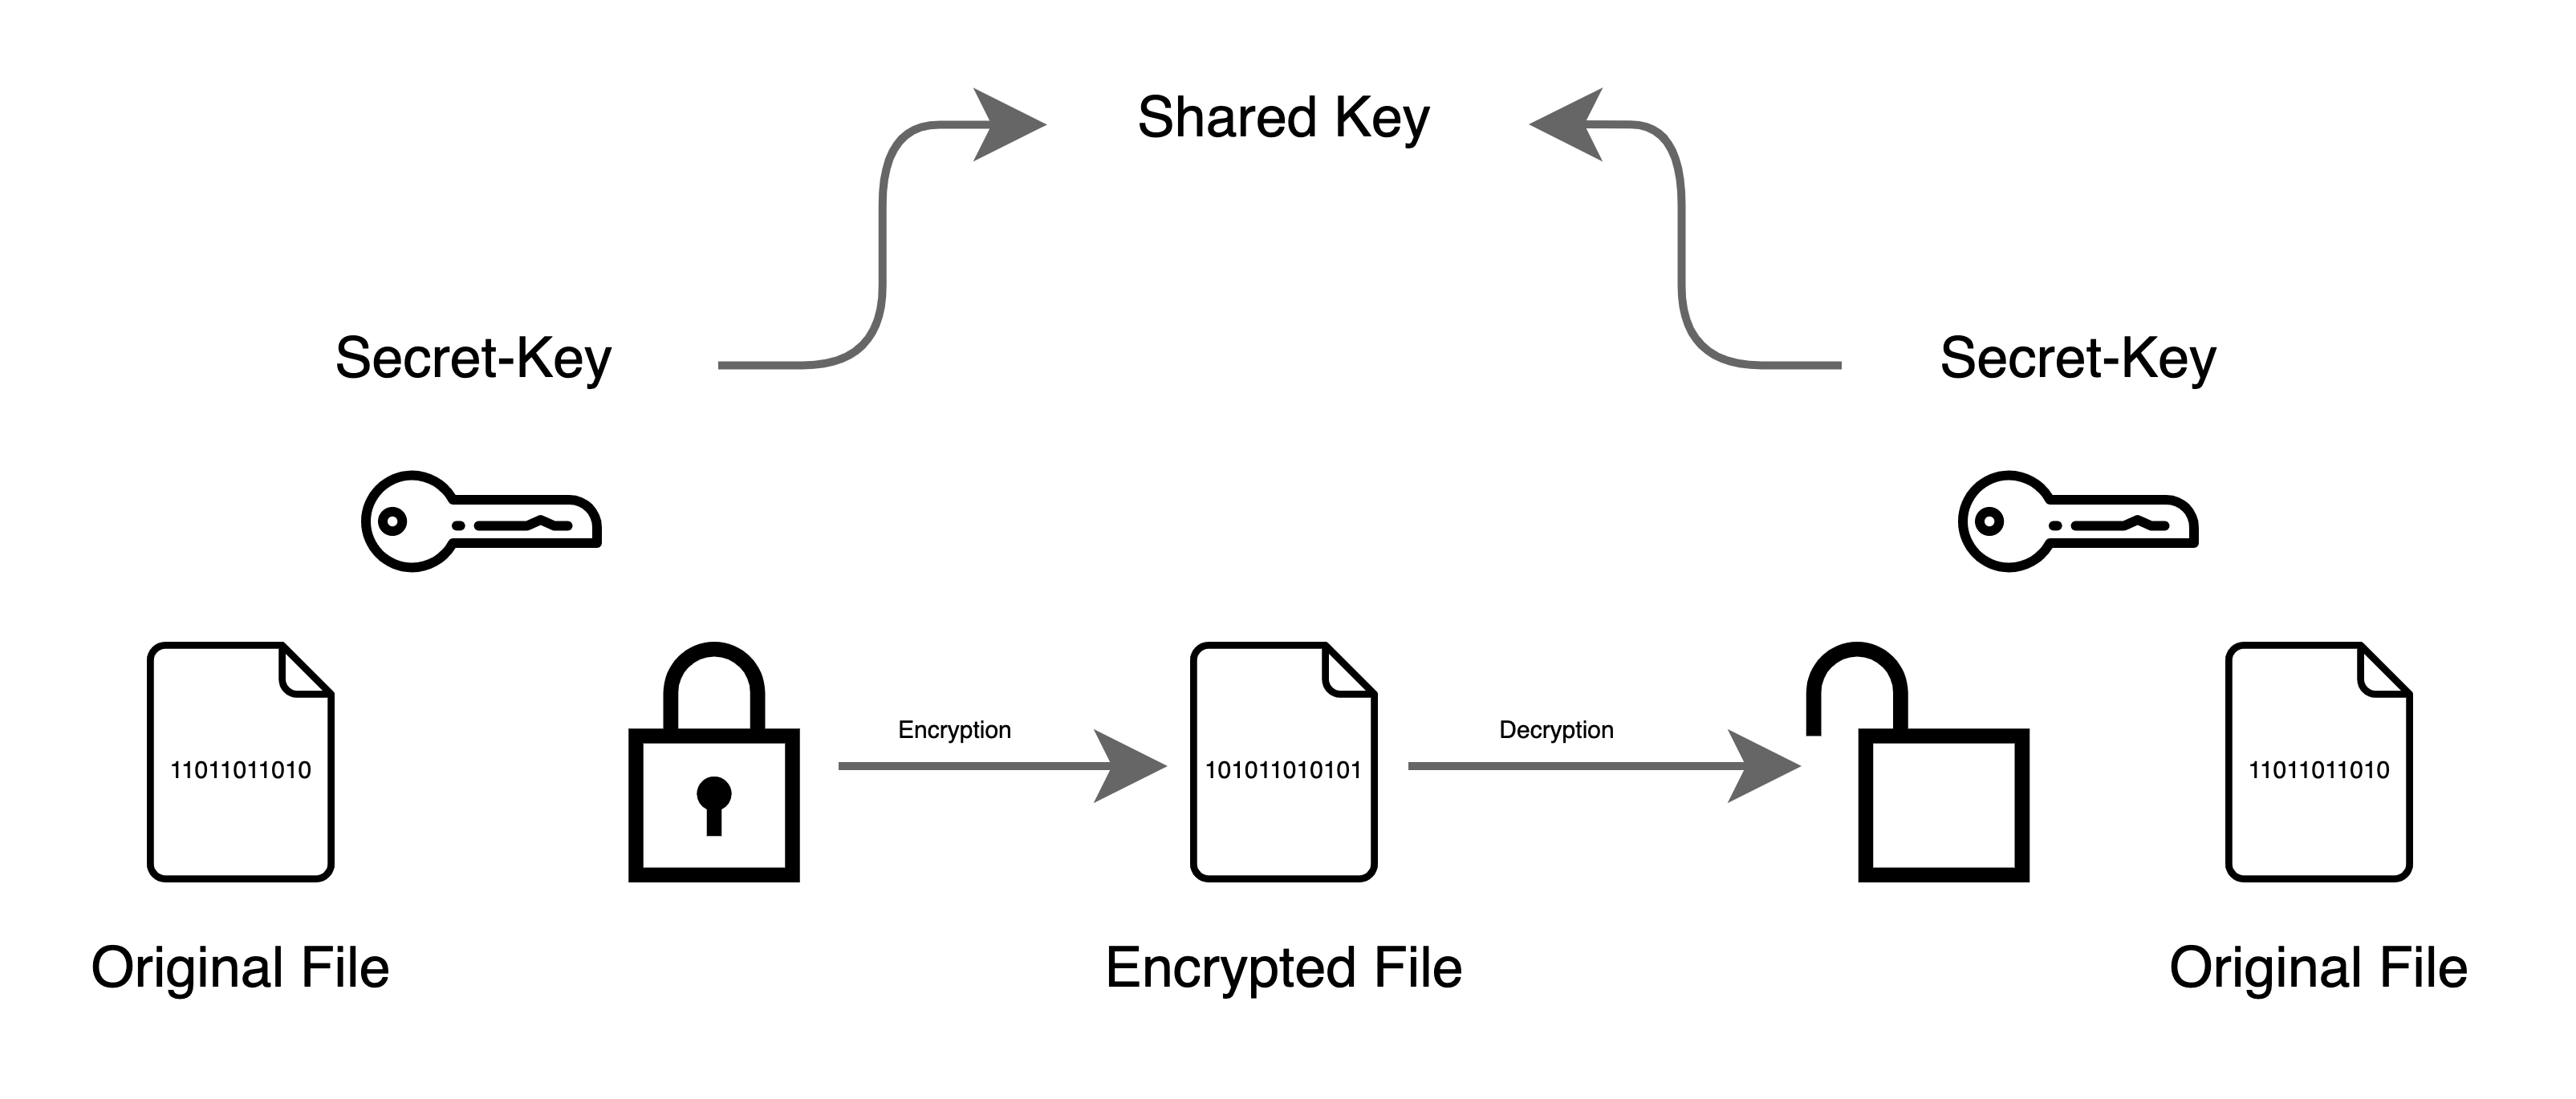
\includegraphics[width=10cm]{aes}
\caption{Symmetric Encryption}
\end{center}
\end{figure}

Viral media contents are encrypted using the Advanced Encryption Standard (AES), also known as Rijndael is a specification for the encryption of electronic data \& information established by the U.S. National Institute of Standards and Technology (NIST) in 2001. The algorithm described by AES is a symmetric-key algorithm, meaning the same key is used for both encrypting and decrypting the data. AES is the first publicly accessible cipher approved by the U.S. National Security Agency (NSA) for encrypting top secret information. AES encryption is used in our daily life mobile communications which is responsible for a large amount of security of our personal data, it is the most commonly used secure cryptographic algorithm.\\

The major reason why Viral makes use of symmetric cryptographic algorithm for securing user's data is due to the threat of quantum supremacy. If quantum computers go mainstream most encryption used in emails, secure messaging, banking services will be compromised and will be subjected to attacks. While an encryption algorithm is basically a math problem that involves a large number of bits making the most common attack (bruteforce) requiring a immeasurable amount of computing power to find the possible combinations to decipher the encrypted data, the possibilities to bruteforce are finite which puts a quantum level computing as a threat to weak encryptions that cannot be cracked by classical computers.\\

There are currently countable quantum algorithms that posses a threat to current cryptography security. Some are
\begin{enumerate}[leftmargin=+0.2in]
\item \textbf{Shor's Algorithm} : Originally discovered by American Mathematician Peter Shor in 1994 is a quantum computer algorithm for finding prime factors of an integer. It can target asymmetric cryptography algorithms like RSA, ECDSA, DSA, etc that uses a public-private key pair for encrypting and decrypting cipher texts. The algorithm reduces the time complexity of Integer Factorization and Discrete Logarithm from sub-exponential to polynomial, and targets keys that can have long cryptoperiods. Since, asymmetric encryption standards such as RSA heavily relies on the fact that classical computers cannot find prime factors swiftly, they are secure for now. US National Academy of Sciences, Engineering and Medicine (NASEM) predicted that a powerful quantum computer using Shor’s algorithm would be able to crack a 1024-bit encryption implementation RSA in less than 24 hours.
\item \textbf{Grover's Algorithm} : The Grover's algorithm discovered by Lev Grover, could theoretically weaken the security of symmetric cryptographic algorithms, such as Advanced Encryption Standard (AES). Grover's algorithm could brute-force a 128-bit symmetric cryptographic key in roughly 2$^{64}$ iterations, or a 256-bit key in roughly 2$^{128}$ iterations. As a result, it is sometimes suggested that symmetric key lengths be doubled to protect against future quantum attacks.  In short, Grover's algorithm reduces the brute-force attack time to it's square root, so the attack time for a 128bit AES encryption is decreased to 2$^{64}$, where the 256bit encryption is reduced to 2$^{128}$ which is considered secure.
\end{enumerate}

Since AES-256 is proven to be the best well-used algorithm currently during post-quantum era, Viral encrypts all the user data using 256bit key symmetric encryption. \\


\begin{figure}[H]
\begin{center}
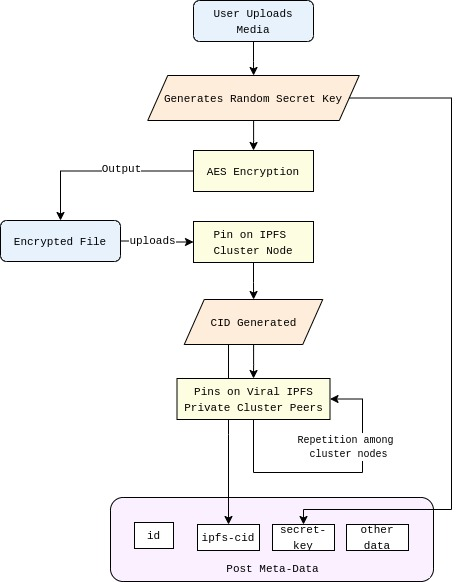
\includegraphics[width=8cm]{encryption}
\caption{Encryption of Media in Viral}
\end{center}
\end{figure}

The steps for Encryption, Media Uploading, IPFS Pinning, Cluster Repetition, Post-Meta-Data Update are given as following
\begin{itemize}[leftmargin=+0.2in]
\item After the media is done for preparation it will begin the encryption process by generating a 256-bit random key.
\item The encryption is done locally inside the device and the encrypted file is generated
\item The encrypted file later hosted to a server that takes the file and pins it to a series of IPFS Public nodes
\item After it is hosted to the Public Nodes via a common IPFS-CID (content-identifier) that CID is pinned on to the IPFS Private Clusters which tracks pins across a cluster of IPFS daemons and uses a leader-based consensus algorithm Raft to coordinate storage of a pinset, distributing the set of data across the participating private nodes.
\item The file is pinned on both Public and Private CLuster Nodes
\item The Repetition of Files among the cluster nodes are determined and configured previously. In summary, the file will be repetitively stored across IPFS-Private-Cluster Nodes. The repetition is monitored by configuring a minimum and a maximum repetition level.
\item After pinning to a single IPFS-Private-CLuster the CID is updated in the post meta-data along with the secret-key which is generated while encrypting the media content
\item The Content is stored in a decentralized, secure and encrypted manner where neither an exploiter nor the developers on Viral can able to view user's content inside publicly available IPFS nodes.
\end{itemize}

\begin{lstlisting}[caption={Post Meta-Data}, numbers=none]

	post id:12 {
    	"cid": "hefTFbifw5P4gXftAwvA4eXQ89f9w7Rv9dCaQRRVQPn93bA",
   		"caption": "This is a sample caption",
    	"gateway": "https://cluster.viral.com/",
    	"secret-key" : "PdSgVkYp3s6v9y$B?E(H+MbQeThWmZq4"
	}
\end{lstlisting}

\textbf{Decryption}\\

Decryption is classified into two categories
\begin{enumerate}[leftmargin=+0.2in]
\item \textbf{Private Account Media Decryption} : Decrypting Private Media which can be only accessed by white-listed user approved followers with maximum privacy and security
\item \textbf{Public Account Media Decryption} : Decrypting Public Media which can be accessed by anyone instantly by openly allowing users to fetch the secret keys.
\end{enumerate}

\textbf{Private Account Media Decryption}\\

\begin{figure}[H]
\begin{center}
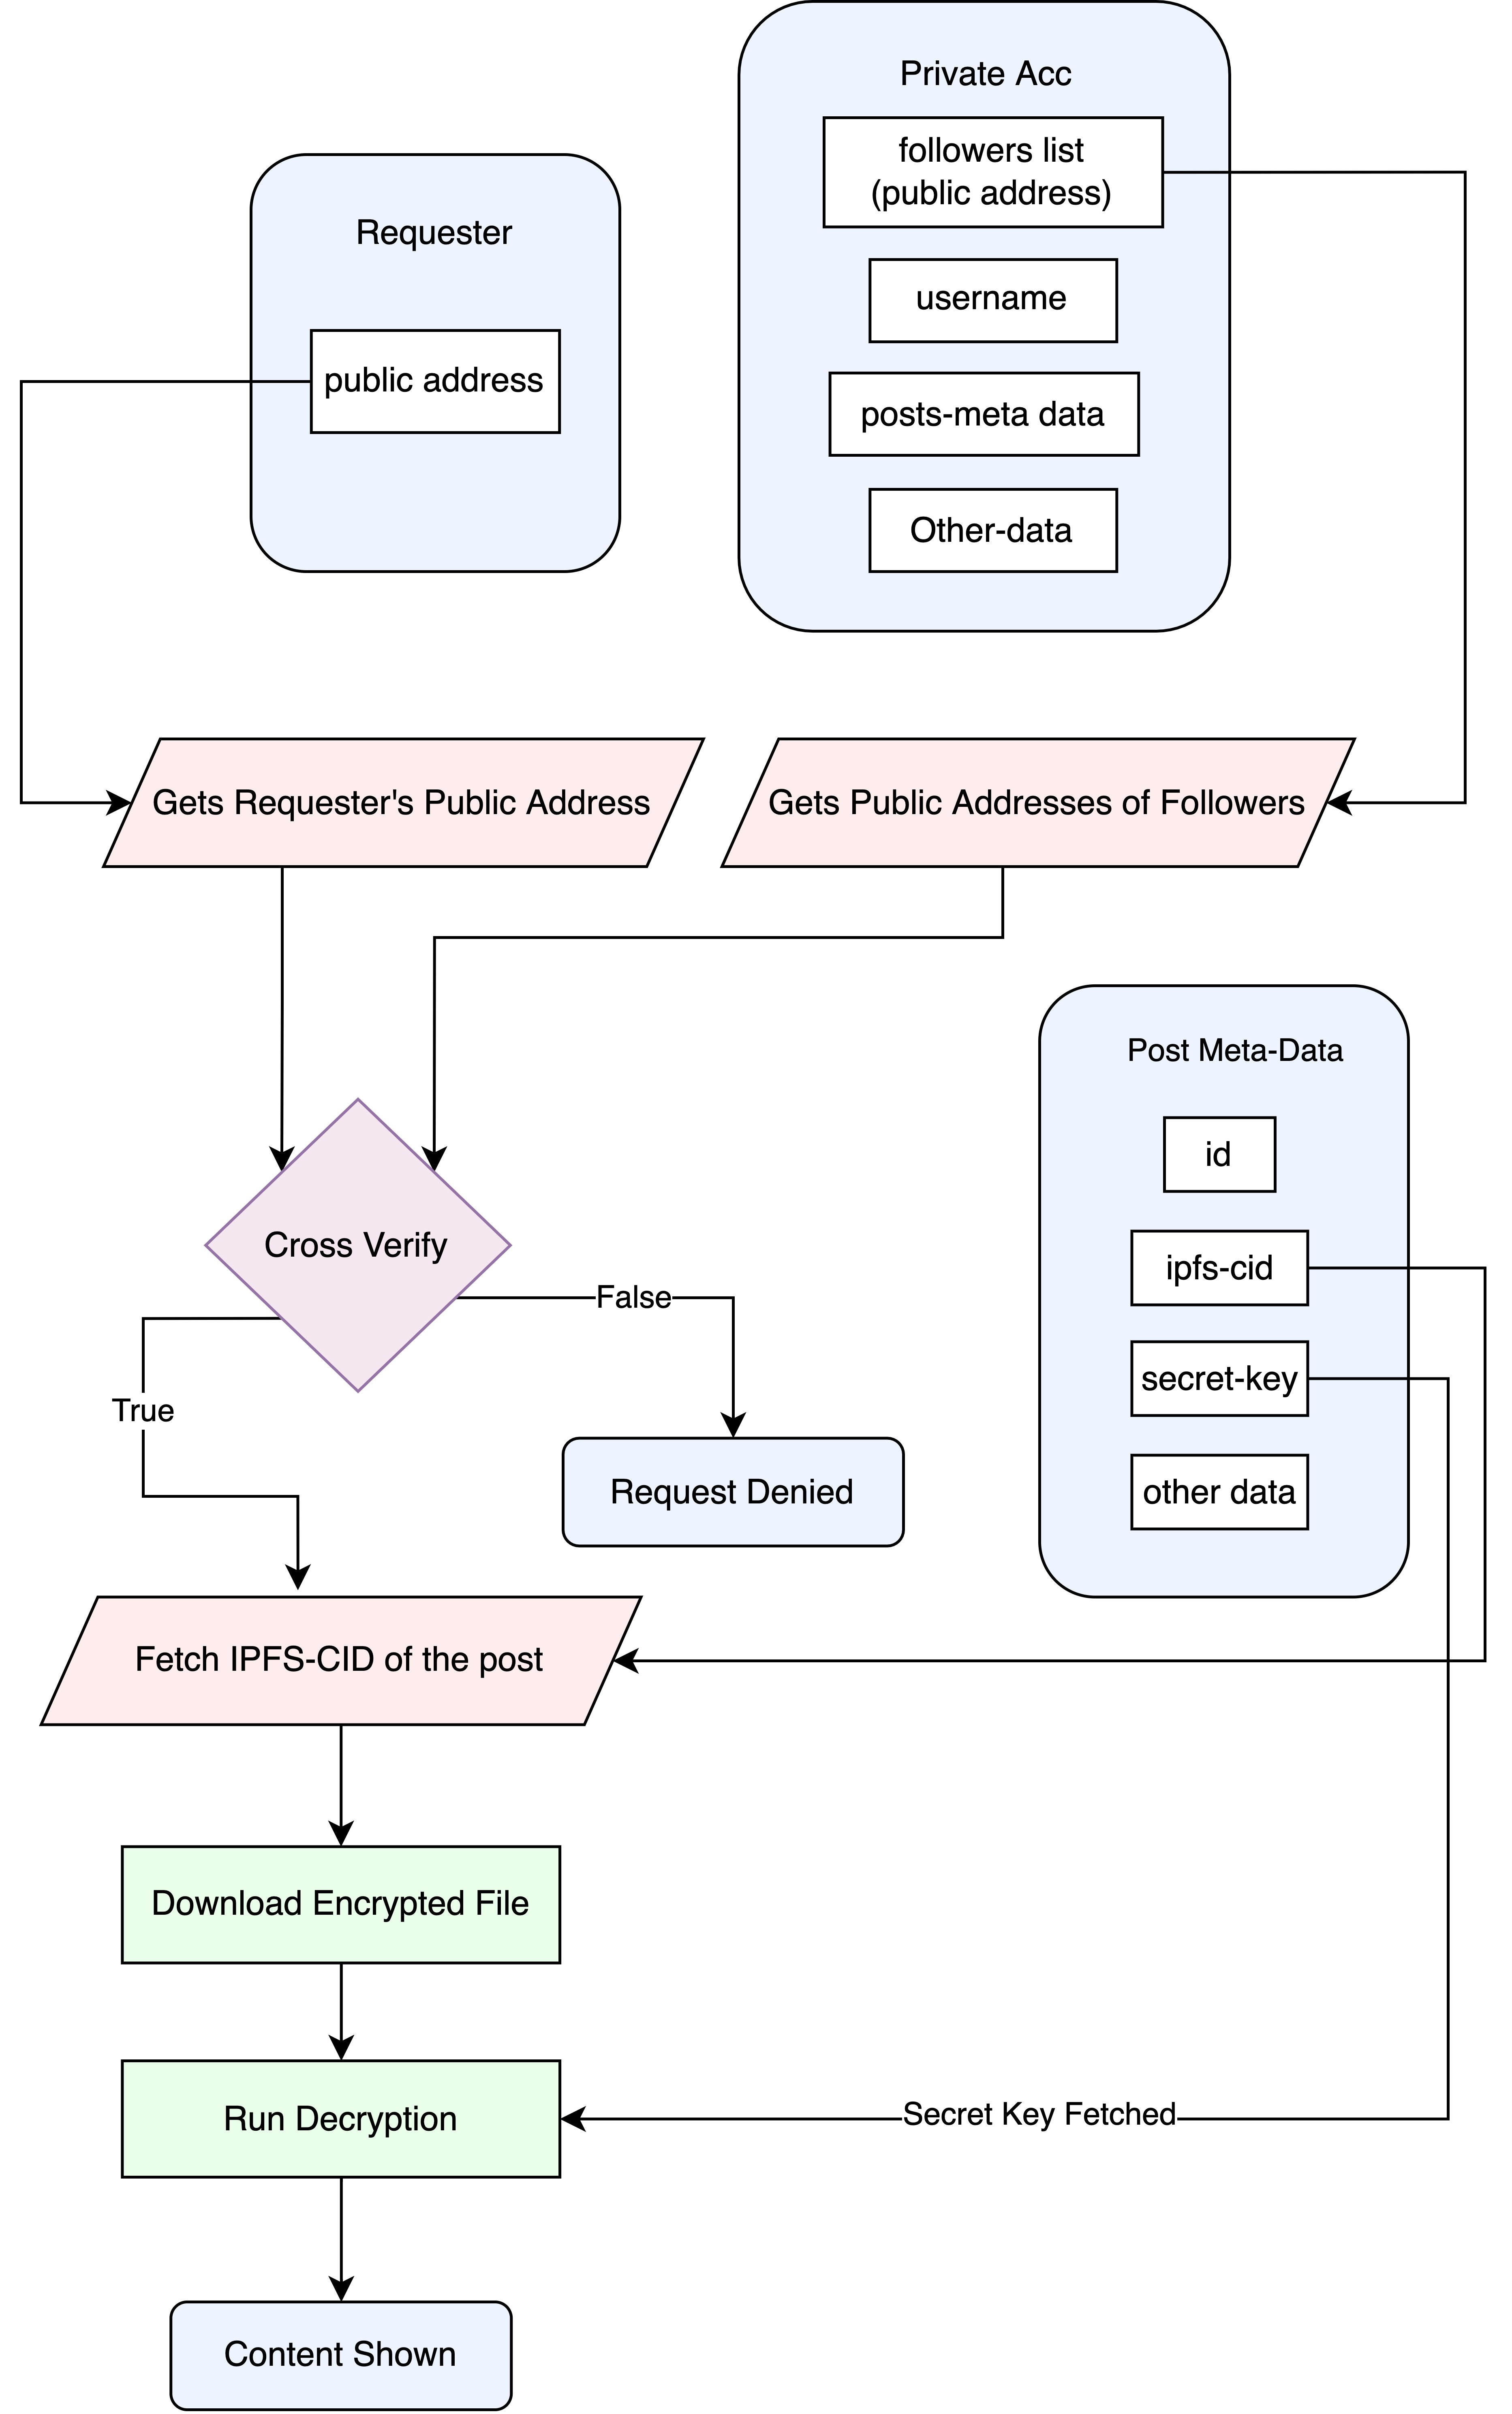
\includegraphics[width=8cm]{decryption-private}
\caption{Decrypting Media of Private account in Viral}
\end{center}
\end{figure}

The Steps on Fetching Public Addresses of content view requester, verification, fetching IPFS CID, downloading and decrypting content is specified below
\begin{itemize}[leftmargin=+0.2in]
\item A Private Account will be limiting it's content access to certain white-listed users that is been approved/accepted by the admin user. Every Viral account shall have a public address which will be added to the white-listed users list.
\item The Public address of the Requester shall be fetched and cross verified with the white-listed user list of the private account. Only the white=listed user will be able to unlock the private account.
\item The meta data of the posts will be decrypted to the white-listed user and the user shall fetch the IPFS-CID and the secret-key of the encrypted file
\item The file is downloaded and decrypted using the symmetric secret-key and the content is shown
\end{itemize}


\textbf{Public Account Media Decryption}\\

Viral ensures that all the content in the social application is securely encrypted compared to current poorly encrypted social media platforms that takes a stealthy look on to people's content even if the account is configured as private. While Public accounts are not encrypted, the storage of files is done centralized on the entity's server farms. Viral is a decentralized social media service that allows anyone to contribute as a storage node and receive rewards in return for the contribution towards the network. This positively puts a violation of storing individual/organizations data which can be used for multiple exploitation attempts due to the growing adoption on big data, machine learning, artificial intelligence, etc.  Neverhtless Viral needs to encrypt public accounts data/content in the most secure manner for nodes to collectively host as a decentralized open network and also providing trust and security to users data.

\begin{figure}[H]
\begin{center}
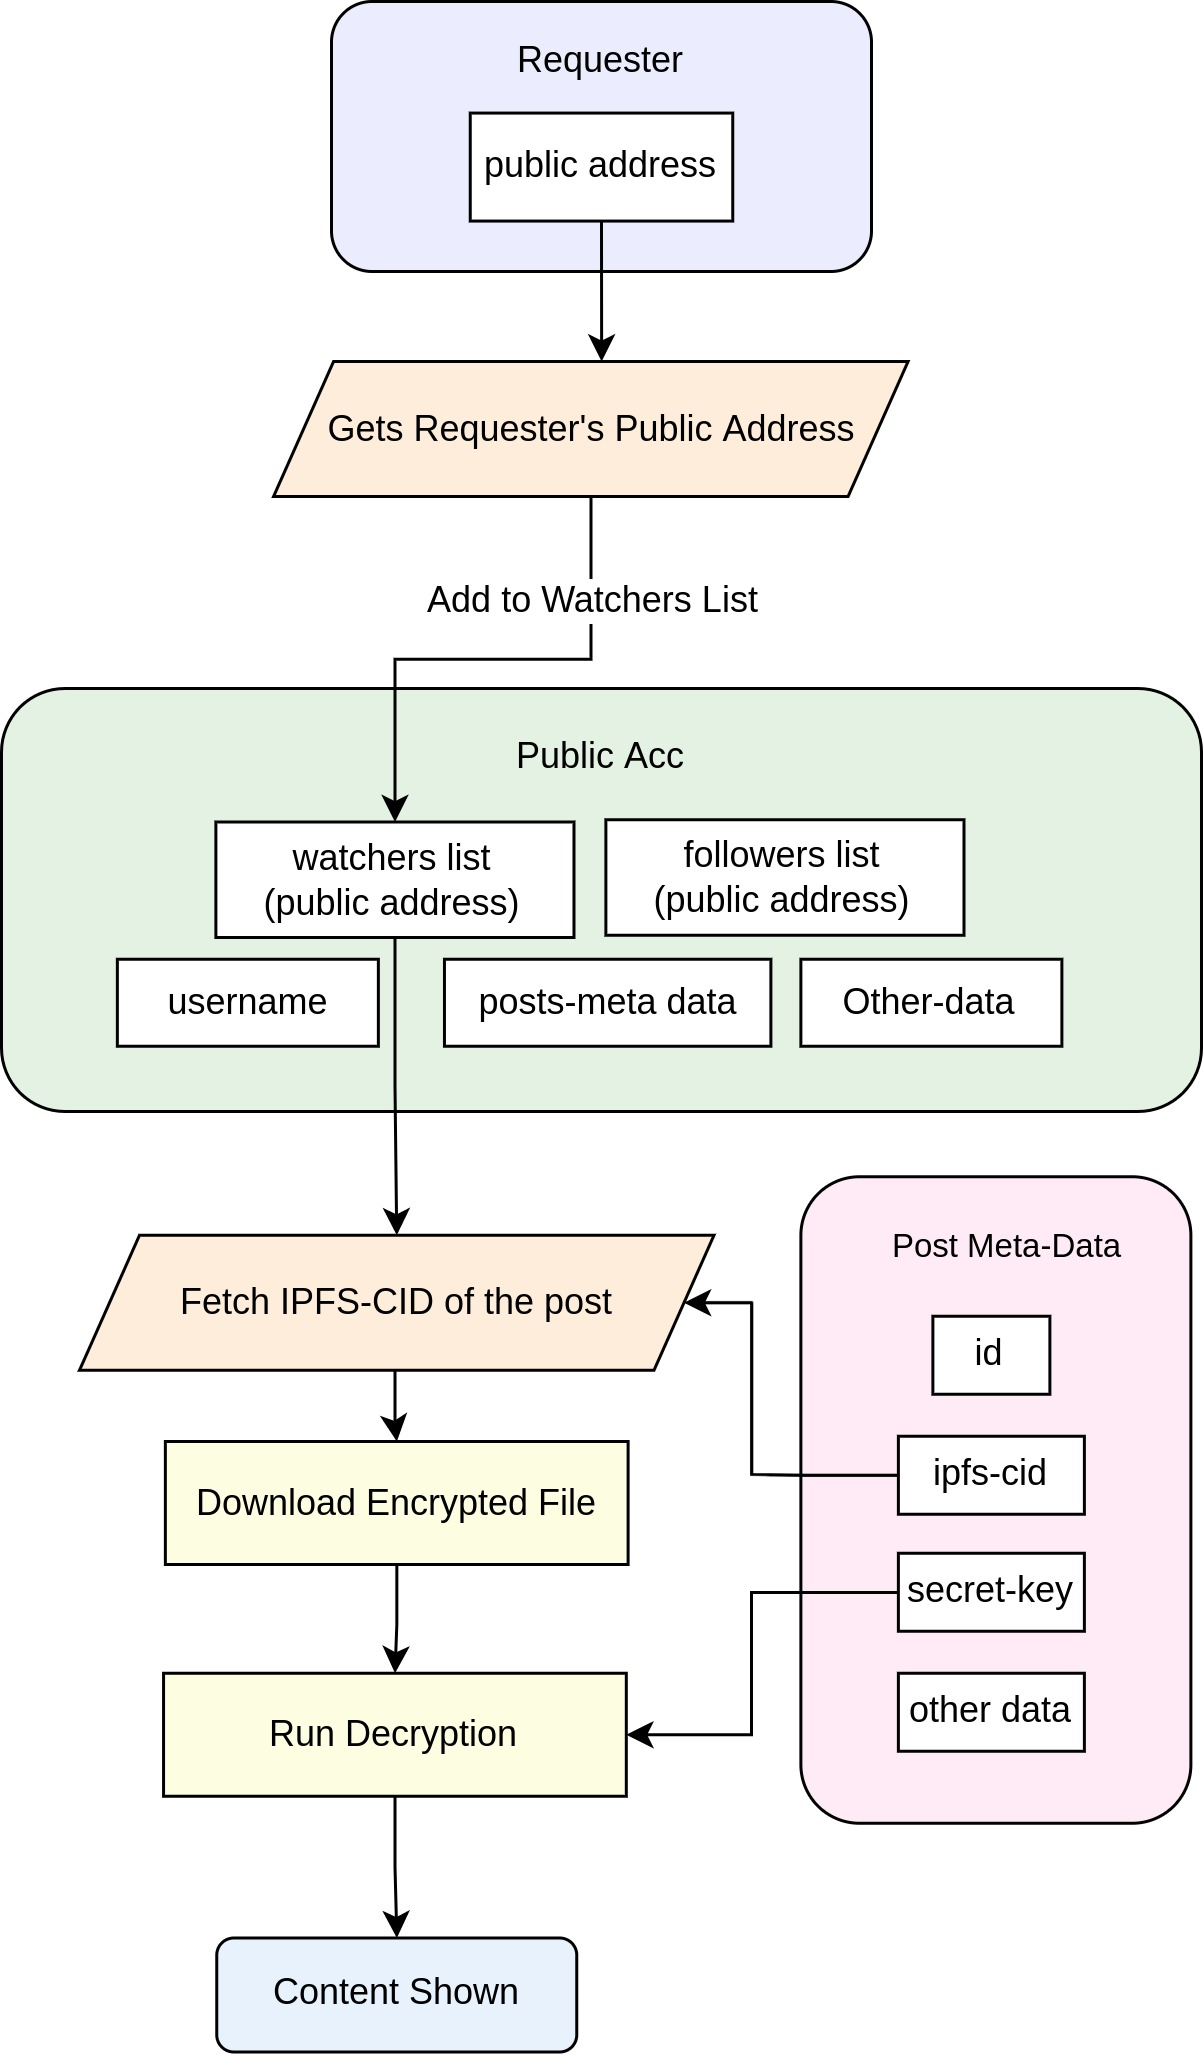
\includegraphics[width=8cm]{decryption-public}
\caption{Decryption Media of Public account in Viral}
\end{center}
\end{figure}

The process of decrypting a public account post is done by maintaining a real-time white-list of users public addresses called "Watchers-list". Viewer's public addresses shall be added in the watchers list to fetch the cid and the secret-key from posts that can decrypt the downloaded content. This way we can ensure the exact security we have in private accounts in public accounts as well.\\


\textbf{2. Chats and Private Messages}\\

For Chat-based encryption, Viral uses \textbf{public and private key} encryption method. Viral Chat is an Offline-First chat messenger which doesn't comprises of centralized cloud-based servers involved in storing messages which can potentially trigger breaches. Every single message is encrypted and can be only decrypted by the receiver.\\

\begin{figure}[H]
\begin{center}
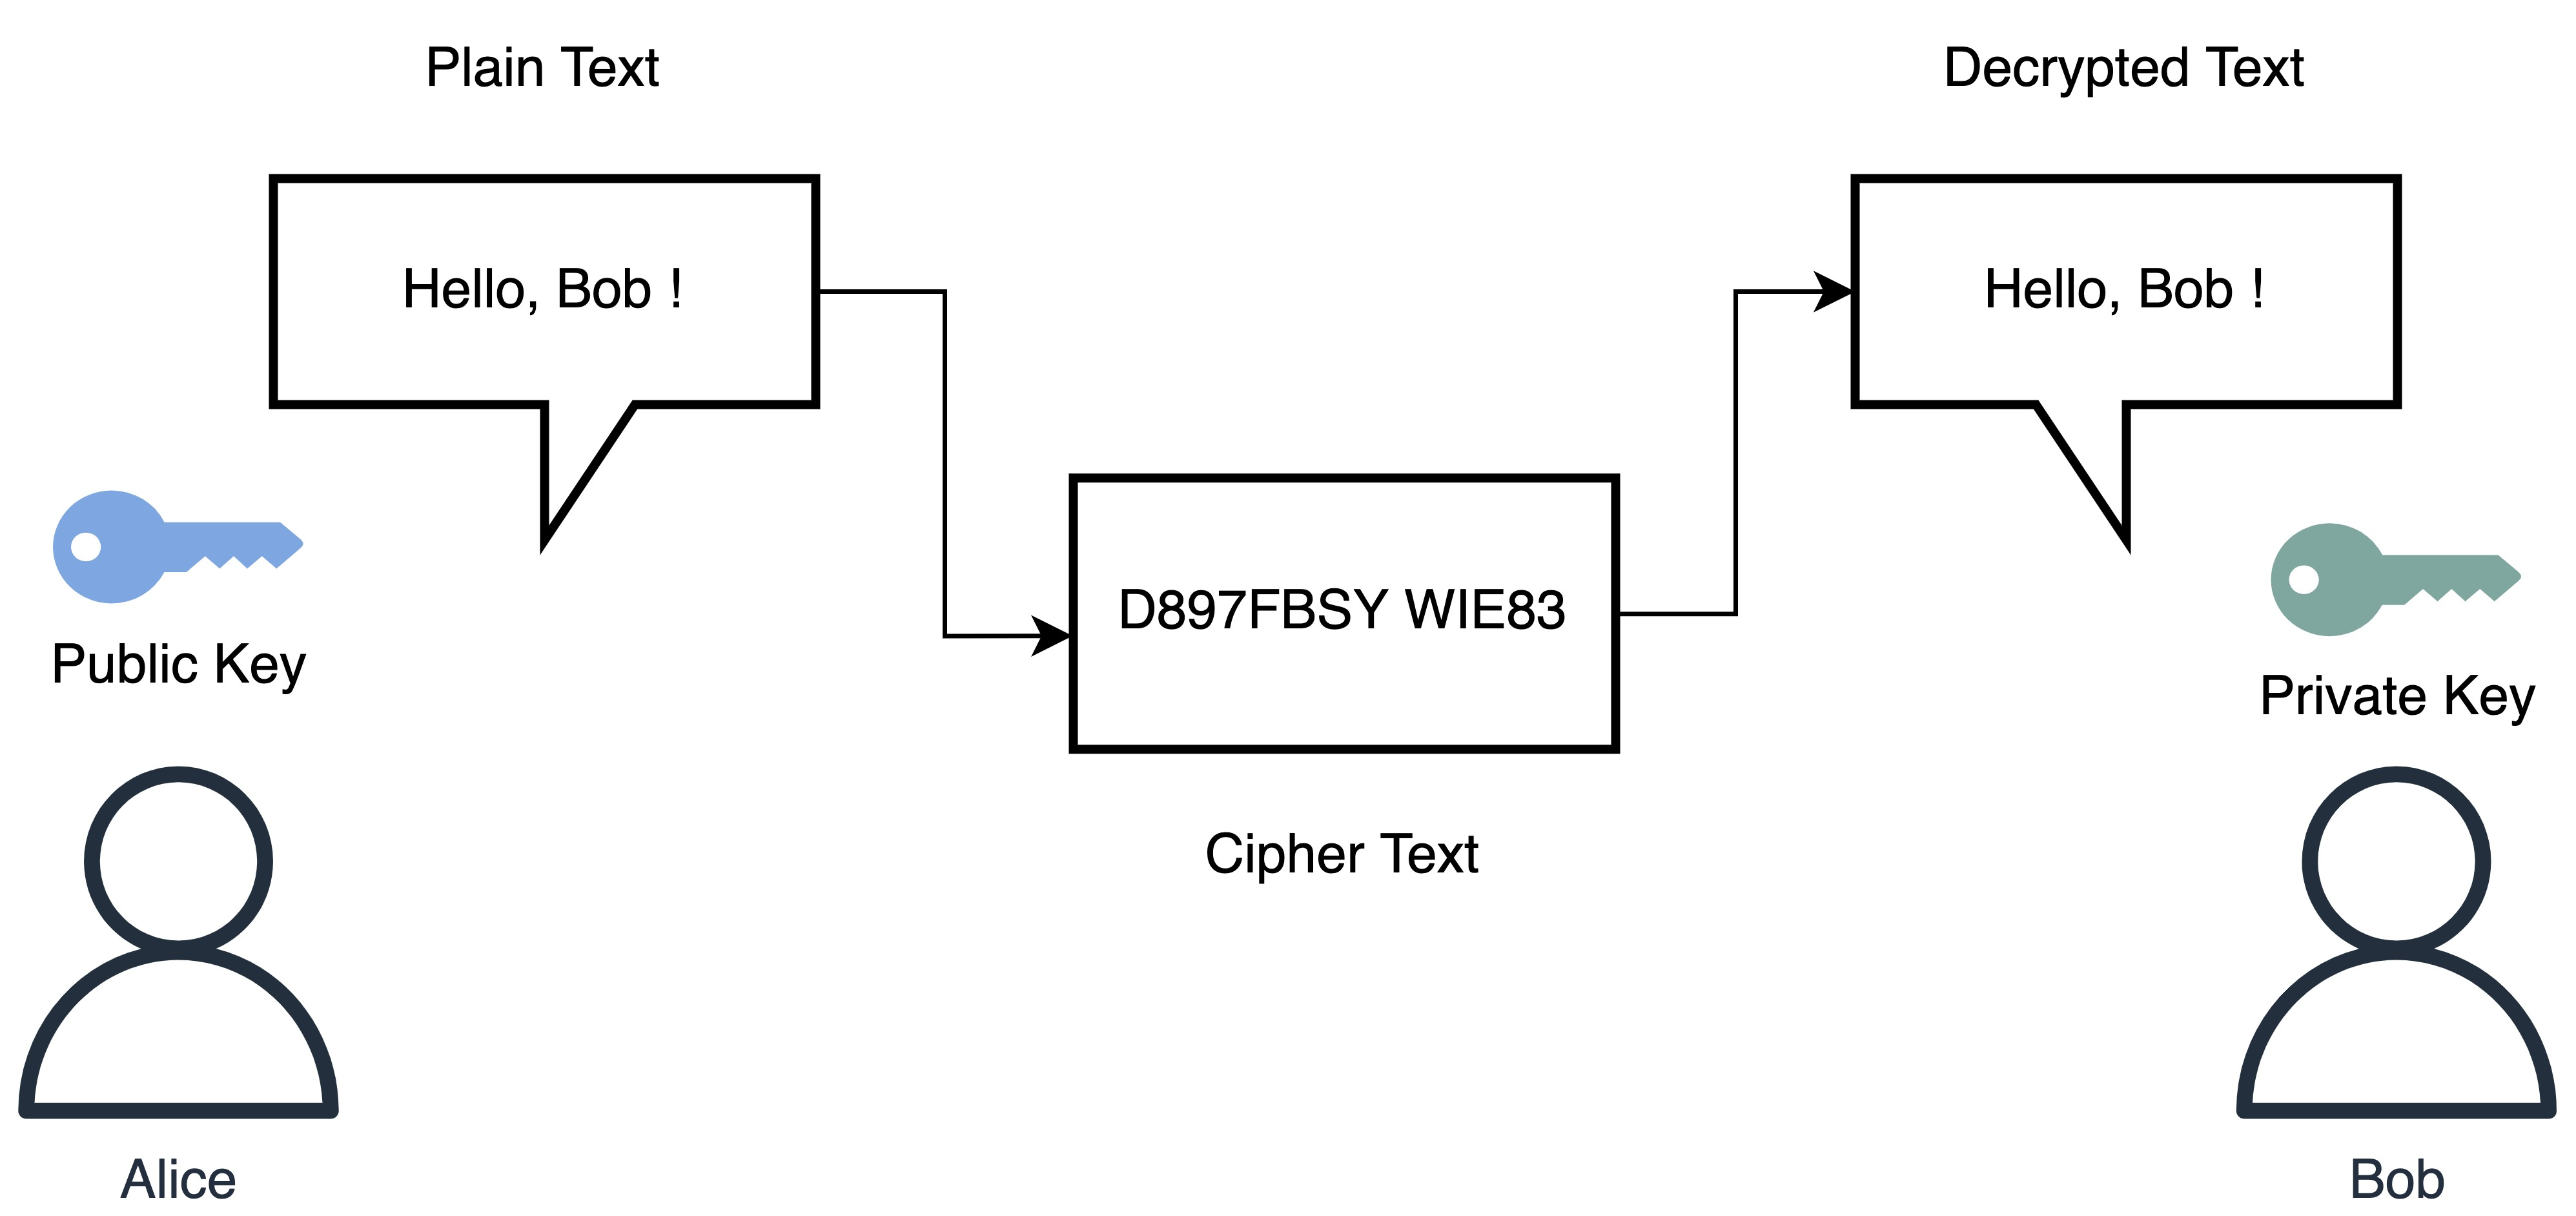
\includegraphics[width=9cm]{chat}
\caption{Asymmetric Chat Encryption}
\end{center}
\end{figure}

External Links : \hyperlink{https://youtu.be/-SiLnaSDkh4}{GunDB Explanatory Video}\\

\textbf{3. Interests of User}\\

Users\textsc{\char13} interests will be \textbf{saved locally} on their devices ensuring full privacy of personal data.\\

\textbf{4. Chat Backup}\\

Since Viral is a \textbf{Offline-First Chat} messages will not be stored in cloud. To Backup messages Viral will offer \textbf{cloud options} such as Google Drive/Dropbox where you can securely encrypt and save your \textbf{backup}. While Migrating to another mobile we will be providing a feature to transfer existing messages/interest to your new device.\\

\textbf{Phase 2 Development}\\

We will be focussing on Quantum Resilience of all media encryption used in Viral while commencing the Phase 2 of Development Roadmap\\

\subsection{TOR/VPN Anonymity}

Viral will be a safe haven for anonymity, privacy, and security in eliminating the tracing of users\textsc{\char13} identities by exploiters . Users can benefit from TOR and VPN Routing Features built in our Decentralized application to hide their IP address and go fully anonymous.\\

TOR routes you through several additional nodes while encrypted, no one can trace it back to you. VPN will redirect your internet traffic through a secure tunnel, hiding your IP address and encrypting your data in the process.\\

\textbf{Content Delivery}\\

Visualization with changes to minting as NFT\\

\textbf{IPFS Cluster}\\

Visualization of Repetition\\

Addition of Nodes – Trusted Way\\

Phase 2 – Trust less Way (IPFS-VM)\\

\section{Blockchain, Token Ecosystem}

\subsection{Viral Smart Chain – Short Intro}

Viral Smart Chains, is a network of parallel Smart Contract Chains on top of a altered Tangle (IOTA) used for Viral Social network with fully deployed defi ecosystem. Viral Smart Chains aim to provide an easy understandable one-platform for all the non-crypto users who are subjected to higher gas fees, congestion in network, volatility and scattered defi solutions. \\

\subsection{Tangle}

The Tangle (by IOTA Foundation) is a next generation Distibuted Ledger Technology that utilizes a new data structure based on Directed Acyclic Graph. Tangle by contrast, does not consist of transactions grouped into blocks and stored in sequential chains, but as a stream of individual transactions entangled together. To do transactions in the network a participant should need to carry out a small computation work to verify two previous transaction. This makes tangle a linearly scalable ledger by network activity implementing participants/users as miners. Transactions in Tangle are completely feeless where miner incentives/rewards are eliminated by providing validation for their own transaction. Instant confirmations and transaction finality is achieved within seconds with low computation requirements.

\subsection{IOTA Smart Contract Protocol}

IOTA provides an Off-Chain Smart Contract Solution for developers to create multiple-chains on Top of Tangle. Since Ethereum transactions are processed On-chain by every single node on its network, it faces additional congestion, slow transaction time and subject to higher miner fees. IOTA\textsc{\char13}s off-chain smart contract solution makes use of blockchains anchored to the Tangle where the smart contracts are ran and achieved consensus with small set of committee nodes. This achieves a high scalable throughput and immutable records since the states of smart contracts such as Account Balances, Input Conditions and Consequences over time are updated on the Tangle. There are several components to understand more about IOTA\textsc{\char13}s Smart Contracts Protocol. It gives us multi-chain functionality to run smart contracts from different chains which allows a horizontal scaling of blockchains without a need for plasma or side chains.\\

\textbf{Consensus and Validators}\\

IOTA\textsc{\char13}s Smart Contract Chain uses a Byzantine Fault Tolerant \(BFT\) Algorithm, which guarantees consistency and byzantine fault tolerance if less than $1/3$ of nodes are malicious. So the verification process runs on Nodes within a chain committee.The validators of the chain \(Nodes\) form a committee, a bound together closed set of nodes. The committee of the chain can allow new validators and validator nodes to be added or replaced. This also makes the chain itself agnostic to its validators \(the committee\).\\

Only when a supermajority of the validators (the quorum) of a chain reaches consensus, the results get added to the chain where a new state update can be signed, which unlocks the AliasOutput for the chain and produces the next state UTXO which is stored on the Tangle as an immutable record. In summary, the chain\textsc{\char13}s state (data) will be stored on Tangle as an immutable record.The amount of the validators to reach a consensus is configurable for each chain. The committee itself can also be variable in size - from a few nodes up to hundreds of nodes, and each node can be part of many different committees.

\begin{itemize}[leftmargin=+0.2in]
\item \textbf{Validators} – Each Single Node running the Chain
\item \textbf{Committee} – The Group of Nodes running a chain
\item \textbf{Quorum} – Number of Nodes to be in consensus to validate a transaction
\end{itemize}

To know more about IOTA\textsc{\char13}s Smart Contracts : \hyperlink{https://files.iota.org/papers/ISC_WP_Nov_10_2021.pdf}{Whitepaper}, \hyperlink{https://wiki.iota.org/smart-contracts/overview}{Documentation}, \hyperlink{https://blog.iota.org/iota-smart-contracts-beta-release/}{Blogs}\\

\subsection{Viral \& IOTA}

While Tangle with Multi-chain functionality is the future of decentralized applications and scalable contract executions, there is still room for improvements because of developers facing a multitude of disagreements inside the protocol which also applies for running a user-focussed application like Viral. \\

\textbf{Dust Protection}\\

The huge disagreement of the various IOTA Protocols is the Dust protection scheme that requires every wallet to have a returnable deposit of Tangle's native asset IOTA in order to successfully transfer various tokens both fungible and non-fungible. In simple terms if a user would want to hold a Non-Fungible-Token in his/her wallet, the user should have a deposit of a certain IOTA coins. This dust protection scheme is introduced to avoid bloating the distributed ledger's size due to fee-less micro-transactions. By eliminating fees the utility for the native asset will decrease if various tokens are being constantly deployed. Viral users are aimed to be common social media users who may not able to deposit a certain IOTA to mint NFTs, send Viral Coins (assuming it's on Tangle) to their friends and family. The Dust protection scheme of the new tokenization framework avoids the usage of IOTA Foundation's Smart Contract Protocol due to Viral's fundamental vision of dissolving preplexing rules of using a crypto wallet and democratize into a simple solution in blockchain applications that feel the same as current simple web 2.0 applications.

\subsection{Viral - Side Tangle}

During disagreements and inability to change the native protocol due to lack of votes, developers fork native block-chains to run a separate block-chain with added functionality that dissolves the disagreement by bringing required changes to the forked(new) protocol. While forked block-chains takes a snapshot of user's balances until a certain block number in the native protocol to convert current coins into newly forked coins that's circulated. Some forks doesn't take snapshots but only forks the source-code to bring necessary changes to the protocol and run independently starting from the genesis block. Since dust-protection scheme of the tokenization framework is a huge concern for a seamless usage of the Viral Application, a source-code fork of the Tangle and the ISC is intend to happen with added functionalities that tie up with the vision of a non-complex crypto solution for the common people and a better framework for existing problems that IOTA encounters such as dust protection, increasing ledger size, decentralization and security of user's funds on less secure chains on top of Tangle.











\subsection{Viral Smart Chains}

\begin{figure}[H]
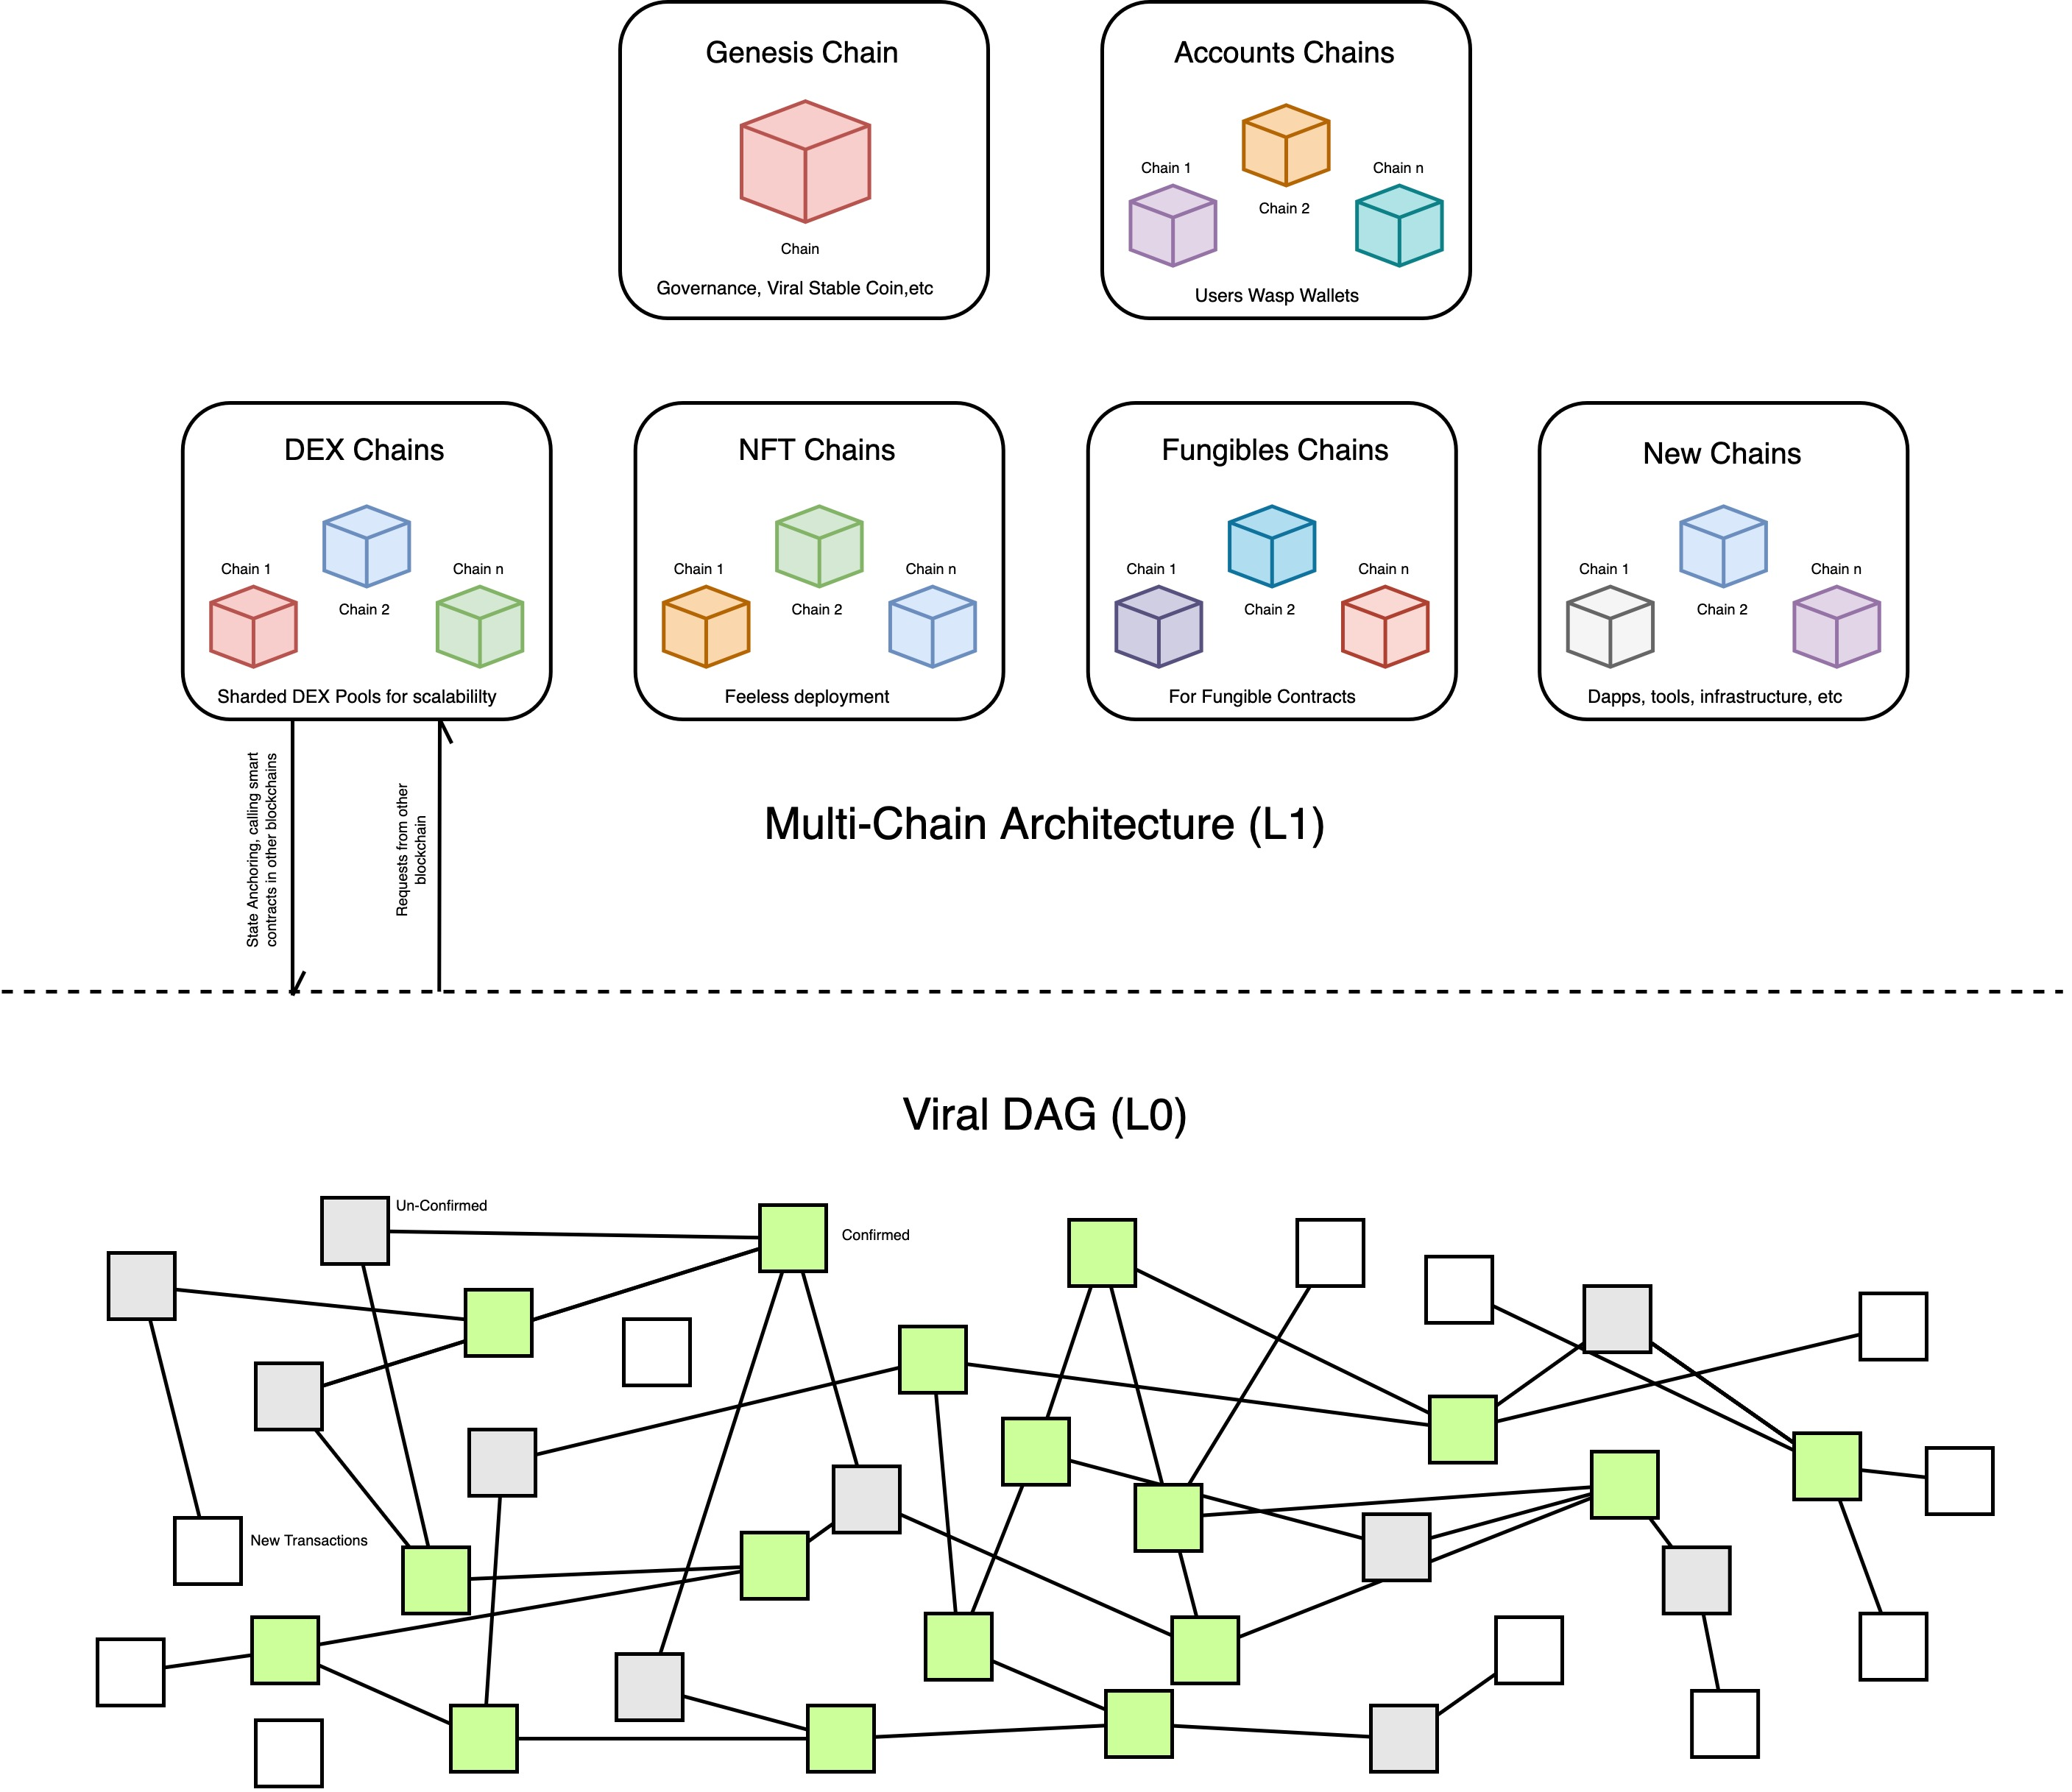
\includegraphics[width=\textwidth]{Architecture}
\caption{Viral Multi-Chain ELI9 Architecture}
\end{figure}

Viral Smart Chains are a family of separate chains anchored to the IOTA\textsc{\char13}s Tangle where each chain can communicate with each other via intermediary L1 Value Tangle.\\

\textbf{Viral's Approach}\\

A Single chain will seem complex for setting different fees for different actions on the blockchain i.e Smart Contract Calls/Deployment, Sending Tokens to other Address, etc. Viral\textsc{\char13}s approach is to bring multiple chains categorized by its purpose to serve the Viral Application with fee structure thereby also creating separate chains to provide zero network fees for minting NFTs on Viral App (ERC721 and ERC1155) while rewarding the validators of all Viral chains (including zero fee chains) from the miner pool (total collected fees of all chains) based on validator\textsc{\char13}s total validated transactions for the day through an automated smart contract.\\

\textbf{Family of Chains}

\begin{itemize}[leftmargin=+0.2in]
\item \textbf{Genesis Chain} : Initialization of First Chain with Viral Coin and Stable Coin Deployment with Smart Contracts that defines governance, fees, etc\\

\item \textbf{Accounts Chains} : For Every n number of active Viral Wallet users a new general chain is deployed. These chains are used to store user funds and create new accounts on the blockchains. So Users can do intra and inter chain transactions with high throughput and flexible scaling.\\
\end{itemize}
\textbf{De-Fi Chains}\\
Smart Contract Deployment Chains specifically for categorized DApps
\begin{itemize}[leftmargin=+0.2in]

\item \textbf{DEX Chain} : Running smart contracts for Viral Wallet\textsc{\char13}s Decentralized Exchange

\item \textbf{ERC20 Chain} : To Deploy new ERC20 Tokens that can be transacted between chains and accounts

\item \textbf{Viral NFT Chain} : Feeless Viral ran Smart Contract Chain specifically to deploy user\textsc{\char13}s NFTs on-chain

\item \textbf{ERC721/115 Chain} : To deploy new Non-Fungible Tokens for other platforms outside the Viral Application

\item \textbf{Marketplace Chain} : To create smart contract based marketplaces for NFTs and much more

\item \textbf{Viral DAO Chain} : For Viral DAO Governance contracts

\item \textbf{Other Chains} : For creating Dapps for lending, asset tokenization, yield farming, tools and infrastructure, etc
\end{itemize}

\textbf{Consensus}\\

ISC Chains uses a BFT consensus where 


\textbf{Validators}\\

Viral Chains will require validators to stake their Viral Coins in order to participate in the network for validating transactions. Chance of validating transactions depends on the amount of coins a validator is stakes. Participants who stake more Viral Coins will be most likely to be chosen to add more blocks. When a transaction is validated and attain consensus by the quorum of validators (Read IOTA Protocol), the state of the transaction/smart contract will be recorded in the Value Tangle\textsc{\char13}s UTXO Ledger which makes the state immutable and impossible to fork. The Transaction will be secured by the validators inside the Viral chain and also the L1 UTXO Ledger.\\

\textbf{Permisionless Validators}\\

\textbf{Wasp Nodes}\\

\textbf{Immutable State Anchoring}\\

\textbf{Core Chain Contracts}\\

\textbf{Chain Ownership}\\


\textbf{On-Chain Accounts}\\





\textbf{Fees}\\

Viral Smart Chain is built primarily to ease the need for gas-based transaction fees like other smart contract blockchains. Transaction fees are only leaved as a fixed percentage as transfer fee in Viral Smart Chains for Sending, receiving tokens between accounts and smart contracts. Transfer fees are fixed at 0.05\% of transfer value of the tokens paid in Viral native coin. The minimum fee is capped at \$0.0005 of the fiat value of Viral Coin which is determined using price oracles. While these fees aren't set for all the Viral Smart Chains, different blockchains served for different purposes will require different fee model. Fee model can be intialized in each chain while deploying the governance core-contracts. Such fee model is proposed below\\

\textbf{NFT Chains}\\

Currently on popular smart contract blockchains such as Ethereum, Polygon the amount of gas required for a transaction is determined by the demand for the transaction to be included, regardless of what type of transaction it is where it is dynamically adjusted based on number of user\textsc{\char13}s interacting with the network at the time.\\

This brings us to an effect that a single blockchain cannot set certain fees or eliminate gas fees for a particular type or category of a transaction regardless of it\textsc{\char13}s nature i.e, smart contract, account transfer. Multiple parallel state blockchains can solve this issue by altering few blockchains as permissioned for a certain use cases and can make it feeless without hindering the other fee-based chains.\\

Viral\textsc{\char13}s aim to democratize NFT to the masses and bring massive NFT Adoption we will be running separate zero-fee chains for deploying ERC721 and ERC1155 Token directly from the Viral Application. The Validators for the chain will be open to join the network where they\textsc{\char13}ll be rewarded from the miner pool (total fee collected) based on the total transactions they validate in a day.\\


Development

\begin{lstlisting}

      _Root_

      - _Initialization of the chain_
      - _Deployment of new contracts_
      - _Registary of contracts_
      - _Chain ownership management and Access control list_
      - _Fee management_

      _Accounts_

      - _On Chain ledger accounts_
      - _Securely moving tokens between accounts_
      - _Ensuring consistency of the on-chain ledger_

      _Eventlog_

      - _Keeping timestamp immutable log of On-Chain events_

      _Blob_

      - _Keeping registry of Binary objects of arbitrary sizew_

      _Configuration of Committee and quorum_

      _Wasp Nodes_

      _EVM Plugins_

      _Configuring Fees_

      _Smart Contract Deployments_

      _State Updates on Tangle_

      _Multi-Chain Integration_

      _Core-Contracts_

\end{lstlisting}

\subsection{Token Ecosystem}

\subsubsection{Viral Coin - Native Token}

Viral Coin is the native currency, a digital coin that does all the operations inside the Viral Smart Chains. It is used to store value, send and receive funds within the Multi-Chain Viral Blockchains. Viral Coin is used for paying fees inside the network, staking, governance, rewards and much more.\\

\subsubsection{Viral Stable Coin}

Viral Stable Coin is a sub-native token, an algorithmic stable coin pegged to the US Dollar that is widely used in the Viral Application for sending and receiving tokens across users wallets. Due to constant volatility of the crypto market there is a barrier for the common people and businesses to get into cryptocurrencies. As Viral\textsc{\char13}s aim to become the one-stop crypto solution for the masses we are providing a way for the user\textsc{\char13}s to automatically transact in Stable Coin without any complex need for swapping their current tokens. In Short, when an user transact in Viral Coin, he can opt to send the receiver viral stable coins to avoid depreciation of the asset while transacting.\\

As far as we know there are several stable coins are in the market 1.Fiat-Peg Centralized, 2.Crypto Collateral 3. Algorithmic. In our case we can take 3 coins 1. USDC 2. DAI 3. AMPL. USDC maintains the peg but holds the funds on its reserves centralized which comes with its demerits. DAI aims to maintain the peg using collateral of several crypto coins, in which USDC hold the reserve of more than 50\% of the DAI\textsc{\char13}s crypto backing, which also makes DAI a centralized cryptocurrency. AMPL is an algorithmic stable coin which maintains it\textsc{\char13}s peg by contracting and expanding it\textsc{\char13}s supply of tokens to achieve stability, this achieves true decentralization but fails to operate swiftly for sudden price movements due to it\textsc{\char13}s rebase function ran in a stipulated time and also rebases in a slow, long way which takes upto a week after a sudden price movement. This is where most crypto projects fail to provide a decentralized stable currency for the masses.\\

Terra blockchain is the most successful running algorithmic stable coin which maintain its stability by changing the stable coin\textsc{\char13}s supply by burning and minting it\textsc{\char13}s native token LUNA. In better words, when Terra (Stable Coin) demand increases to more than \$1, Luna (Native token) will be burned and New Terra tokens will be minted, where increase in supply of tokens resolves the demand and maintains the peg of the stable coin and vice versa. Viral Stable Coin adopts the algorithmic stable coin algorithm used in many of Terra\textsc{\char13}s stable coins.\\

Viral Coin and Viral Stable Coin will be the two primary coins in the Viral Social Platform. The supply and demand of Stable Coin is always balanced by making Viral Coin as it\textsc{\char13}s variable counterweight that absorbs it\textsc{\char13}s volatility.\\

\textbf{1 VSC - \$1 (Expansion)} : When Viral Stable Coin trades at a price that is high relative to it\textsc{\char13}s \$1 peg i.e., \$1.15, the demand for VSC is higher than the circulating supply. To bring the peg back to \$1, the supply of VSC should be increased to balance the demand. During Expansion State trading bots will mint VSC by burning VRL, which has an effect of lowering Viral Stable Coin Price (by expanding the supply) and increases the Viral Coin price (by reducing it\textsc{\char13}s supply). The smart contracts will trade until the price peg of 1 VSC = \$1 is achieved.\\

$Formuka for Expansion$\\

\textbf{1 VSC - \$1 (Contraction)} : When Viral Stable Coin trades at a price that is low relative to it\textsc{\char13}s \$1 peg i.e., \$0.95, the demand for VSC is lower for the circulating supply. To bring the peg back to \$1, the supply of VSC should be decreased to balance the demand. During Contraction State trading bots will burn VSC and mints VRL, which has an effect of increasing Viral Stable Coin Price (by reducing it\textsc{\char13}s supply) and lowering the Viral Coin price (by expanding it\textsc{\char13}s supply). The smart contracts will trade until the price peg of 1 VSC = \$1 is achieved.\\

\textbf{Viral Stable Trading App}\\

High Frequency trading cannot be run using automated smart contracts to maintain price peg of Viral Stable Coin. Users can stake their Coins, run automated arbitrage trading and receive profits using the Viral Stable Trading Application a separate application to maintain the peg of Viral Stable Coin\\

Users will be able to stake both coins VRL and VSC proportionally to a smart contract in the mobile app which process all transactions of burning and minting VRL for VSC automatically without the need for user signature and receive profits from arbitrage opportunities by minting and burning the coins to balance the volatility. The Smart Contracts will add and subtract coins on each pools to maintain stability.\\

\subsubsection{Wrapped Tokens}

To acknowledge the tokenized economy Viral will bring popular cryptocurrencies such as Bitcoin, Ethereum, Dogecoin, etc into the Viral Smart Chains using wrapped token method. Since interoperability of blockchains are not possible (blockchains cannot talk to each other), centralized exchanges are used to exchange cryptocurrencies between each other using order books where the exchanges act as a custodian maintaining the user’s crypto holdings (E.g.: Bitcoin to Ethereum). To eliminate centralized processes, tokenization of other blockchain coins are introduced. Original Tokens will be reserved in it's native blockchain and a copy of the tokens, new wrapped tokens will be minted (created) on Viral Smart Chains. The wrapped tokens will be 1:1 pegged with the native cryptocurrency and can be used in various de-fi applications. Viral Smart Chain's approach is to develop several wrapped tokens of popular cryptocurrencies for its users to invest and exchange in a decentralized manner.\\

\textbf{Viral Decentralized Bridge}\\

Intro\\
Type of Viral Bridges\\
ERC20 Bridge\\
Abstract\\
List of Cryptocurrencies\\
Mechanisam\\
Flowcharts\\
UTXO Bridge\\
Abstract\\
List of Cryptocurrencies\\
Mechanism\\
Flowchart\\
Conclusion\\
Hence Users can invest in Bitcoin and other popular cryptocurrencies if they want to, without any hassles of other wallet applications or other blockchain wallets.


\section{Viral Pay - Smart Wallet}

From early days of bitcoin, crypto wallets serves the one-stop solution to hold and transfer cryptocurrencies through an easy user experience model. There is so much to crypto wallets other than holding coin. Wallets can send, receive digital money, store NFT collectibles, connects to exchanges and a lot more to be integrated in the upcoming future, probably your one account hub for everything in the internet. In,short wallet applications are a place to store your cryptocurrencies securely. 

\begin{figure}[H]
\begin{center}
\begin{forest}
  forked edges,
  for tree={edge+={-Latex}},
  [Crypto Wallet
    [Non-Custodial
        [Hot Wallet]
        [Cold Wallet]
        [Paper Wallet]
    ]
    [Custodial
    ]
  ]
\end{forest}
\caption{Types of Wallet}
\end{center}
\end{figure}


Wallets are classified into centralized custodial wallets and decentralized non-custodial wallets. Decentralized wallets offer high security and total freedom, while custodial wallets in exchanges comply to regulations. Hot wallets are non-custodial wallets that's always connected to the internet and the blockchain network using various APIs to send, receive, view tokens  easily through a browser or a mobile application. Cold wallets are offline physical wallet devices that stores tokens in a storage device i.e., USB Drive that is secure to over the internet attacks. Viral provides hot wallet services to users through an integrated wallet application inbuilt inside the social application.\\ 

\textbf{Pros of Hot Wallets}
\begin{enumerate}[leftmargin=+0.2in]
\item \textbf{Access assets anywhere} : Hot wallets provide you the ability to access user's digital assests anywhere, using compact mobile/browser applications
\item \textbf{Free to use} : It takes zero cost to create a wallet address and generate private keys to access the wallet
\end{enumerate}

\textbf{Cons of Hot Wallets}
\begin{enumerate}[leftmargin=+0.2in]
\item \textbf{Loss of Private Keys} : Since Non-custodial wallets are decentralized user will hold his private keys and no banks or intermediary custodians will hold on behalf of them. This puts an undeniable risk of losing a cryptographic key or a mnemonic phrase.
\item \textbf{Less Secure than Cold Wallet} : Hot wallets are connected to internet which leaves a vulnerability of potential hacks and threats unlike a cold storage which stores tokens offline.
\end{enumerate}


\textbf{Viral Smart Wallet}\\

Viral Smart wallet is an integrated open-source EVM based hot wallet application that is used to store, send, receive, by \& sell Viral ecosystem of tokens and also used to receive rewards for their contribution towards the decentralized network. Users can create, import multiple wallets and get access to fiat-exchange, decentralized swap pools and zero fee L2 transfers for micro-transactions. \\

\textbf{Create Wallet on Viral}\\




\subsection{Viral Decentralized Exchanges}

Decentralized exchanges (DEX) are a type of cryptocurrency exchange that allows for direct peer-to-peer cryptocurrency transactions to take place online securely and without the need for an intermediary or a custodian, unlike Centralized exchanges. Decentralized exchanges are simply a set of automated smart contracts (code). They establish the prices of various cryptocurrencies against each algorithmically and use “liquidity pools” — in which investors lock funds in exchange for interest-like rewards — to facilitate trades. While transactions on a centralized exchange are recorded on that exchange’s internal database, DEX transactions are settled directly on the blockchain itself. There will be no custodian or any services which need to be maintained by a certain company to run a truly decentralized crypto exchange.DEXs are usually built on open-source code, meaning that anyone interested can see exactly how they work. That also means that developers can adapt existing code to create new competing projects — which is how Uniswap’s code has been adopted by an entire host of DEXs with “swap” in their names like Sushiswap and Pancakeswap.\\

\textbf{Automated Market Makers}\\

An automated market maker (AMM) is a type of decentralized exchange (DEX) protocol that relies on a mathematical formula to price assets. Instead of using an order book like a traditional exchange, assets are priced according to a pricing algorithm.This formula can vary with each protocol. Most AMMs usesa constant product formula: $x  \times  y = k$, where $x$ is the amount of one token in the liquidity pool, and $y$ is the amount of the other. In this formula, k is a fixed constant, meaning the pool’s total liquidity always has to remain the same. Liquidity providers (LPs) add funds to liquidity pools. In return for providing liquidity to the protocol, LPs earn fees from the trades that happen in their pool. LPs deposit an equivalent value of two tokens – for example, 50\% of Token A and 50\% of Token B to the A/B Lquidity pool.\\

\textbf{Pros of AMMs}
\begin{enumerate}[leftmargin=+0.2in]
\item \textbf{No KYC Procedures}: Decentralized exchanges are similar to peer-to-peer exchanges but rather taking from an individual the user can withdraw funds from a trustless liquidity pool that requires no ID verification and other complex processes
\item \textbf{Secure} : DEXs are secure as the funds are withdrawn, deposited and held on-chain through smart contracts that is secure and immutable
\item \textbf{Non Custodial}: Liquidity Providers can provide liquidity and withdraw them whenever they need to, making it a non-custody protocol where user's funds will be held on a smart contract rather than a central custodian.
\item \textbf{Zero Manipulation}: Since user's funds are stored in a trustless manner, the smart contracts cannot freeze any account, transfer data to anyone nor manipulates price like a centralized exchange
\end{enumerate}

\textbf{Cons of AMMs}
\begin{enumerate}[leftmargin=+0.2in]
\item \textbf{Scalability}: Various DEXs are suffered from network congestions which delays the execution of trades. This is been solved by making DEXs on top of scalable high throuoghput blockchains, but the DEXs are limited to the scalability of the blockchain itself and cannot scale on it's own.
\item \textbf{Price Impacts}: Price impact is the influence of user's individual trade over the market price of an underlying asset pair. It is directly correlated with the amount of liquidity in the pool/Automated Market Maker (AMM).
\item \textbf{Limited Functions}: AMM based DEXs offers only to execute buy and sell orders and doesn't offers advanced trading features like limit orders aren't available on current exchanges.
\item \textbf{Volatility}: As price impacts being created, on an illiquid trading pair the volatility always reach new highs to stabilize the constant $k$ in the constant product formula $x \times  y=k$ to satisfy demands. This creates high volatile market while user's only use DEXs go for high liquid, low volatile market.
\item \textbf{Impermanent Loss}: Impermanent loss describes the temporary loss of funds occasionally experienced by liquidity providers because of volatility in a trading pair. Liquidity Providers suffer negative returns comparing to holding tokens outside the pool. Volatility and Price Impacts are the major aspects of impermanent loss. The loss becomes permanent if a provider decides to withdraw their liquidity from the pool.
\end{enumerate}

\textbf{Problem 1 : Price Impacts \& Volatility in AMMs}\\

The difference between the current market price and the price a user will pay to perform a swap in a decentralized exchange is known as Price Impacts. This happens when the ratio of the assets in the pool changes where one asset is more liquid and another is illiquid. When a large swap is conducted a maximum portion of the swapped asset is erased from the liquidity pool, supplying more of the provided asset, to maintain the $k$ of the constant product formula $x \times y=k$ the smart contract will ask for a increased supply of tokens to balance the $k$. This will create a impact on the current price, making the trade much more expensive than centralized trades and spiking the volatility of the pool.\\



For example\\

Two Coins $X$ and $Y$\\


\textbf{Pool Info/Before Swap}:
\begin{itemize}[leftmargin=+0.2in]
\item Before Swap $X$=20
\item Before Swap $Y$=45,000
\item Constant Product $K=X \times  Y$ = 900,000 
\item Before Swap Price $M=\frac{Y}{X}$ = 2,250 
\end{itemize}

\textbf{Trade $n$}: $n$= 9,000 y for x\\

\textbf{After Swap}:
\begin{itemize}[leftmargin=+0.2in]
\item After Swap $Y_n$=54,000 
\item Constant Product ($K$) = 900,000 (Stays Same)
\item After Swap $X_n=\frac{K}{Y_n}$ = 16.666  
\end{itemize}
\textbf{Results}:
\begin{itemize}[leftmargin=+0.2in]
\item Received $X_f={{X}-{X_n}}$ = 3.334 
\item Price paid per X / After Swap Price $M_n={\frac{n}{X_f}}$  = 2,699  
\item \textbf{Price Impact} $P={\frac{M - M_n}{M} \times  100}$ = \textbf{19.95\% }
\end{itemize}


\textbf{Conclusion}:\\

To take 9,000 Y Tokens from XY Pool having 20:45000 Tokens, user have to pay \textbf{19.95\% more} than the market price. \textbf{Market Price = 2,250} , \textbf{User Price = 2,699}\\


Huge price impacts happens only in pools that has less liquidity when a maximum percentage of a token in a pool is withdrawn. These price impacts are being neutralized by arbitrage traders who buys token at lower prices on other exchanges and sell the same token high on decentralized exchanges which will has a maximum price impact, these arbitrage traders will continue to make trades for profits until the market price is achieved. Although arbitrage traders are available to minimize the price impacts, users cannot always wait for the arbitragers to stabilize the pools. DEX aggregators offer users a better solution by buying the token across all pools in order to minimize price impact on each one of them. Instead of spreading the trade over time in a single market, this order executes at once, spread over many possible markets. Aggregators also command substantially higher gas costs than a single trade, similar to splitting trades manually. To conclude there are different secondary solutions that minimizes the price impact through secondary trades (trades after the price impact maximizes), the first trader after it neutralizes will always execute orders with price impacts and slippage of prices while multiple trades happen in the middle.\\

\textbf{Problem 2 : Limited Functions}\\

Order book centralized exchanges offers advanced trading features such as limit orders where traders can bid and ask at different prices from the current market prices. DEXs doesn't offer limit orders and only offers instant market orders with a possible price impact. Order book exchanges are better in terms when it comes to live exchanges and better prices for buying and selling. AMMs has its own benefit compared to order books by providing liquidity at anytime regardless of number of orders.\\

\textbf{Problem 3 : Impermanent Loss}\\

Impermanent loss is the most common loss a liquidity provider experience and a risk of using Automated Market Maker (AMM) based Liquidity Pools. Impermanent loss deals with pairs of the liquidity pools, usually while contributing to a liquidity pool a liquidity provider shall equally provide both tokens according to it's market price that will determine the liquidity providers share of the pool in percentage. For example in a pool of XY Tokens for every X token \$100 tokens of Y should be provided taking Y token as a Stable Coin with Y=\$1, when a LP provide 1:100 worth \$200 to the pool with a final ratio of 10:1000 has 10\% of the pool where the LP will be rewarded extra with the transaction fees (usually 0.3\%) according to the percentage the the LP holds. To represent his liquidity the LP will be offered with LP Tokens of the specific pool which the LP can claim and withdraw his tokens.\\

When trades happens the volatility of the two pairs is a nightmare to LPs due to changes in prices that leads to impermanent losses. Impermanent losses are not permanent until the LP withdraw his pool's liquidity. From the above example after the LP provided XY Tokens with 1X = 100Y if the price of X token appreciates to 1X = 400Y, the ratio of the pool would haved changed to 5:2000 maintaining the constant of total liquidity. When the LP withdraws his tokens from the pool he is entitled to his 10\% of funds withdrawing 0.5X and 200Y which totals to \$400. The LP made a profit of \$200, but would have gained more by simply holding the funds of 1X and 100Y worth \$500. The losses compared to holding and providing to a liquidity pool is often termed as impermanent loss but sometimes will be substituted by trading fee rewards. Effects of huge price volatility and impacts creates impermanent losses of LP's funds.\\

\textbf{Problem 4 : Scalability of DEXs}\\

Decentralized exchanges suffer greater scalability issues during frequent network congestions of blockchains. The scalability of DEXs is directly related to the scalability of blockchains. Without a highly scalable blockchain DEXs cannot prepare for a mainstream adoption where trading volume would increase by radical margins.\\

\textbf{Solution to Current Risks}\\

Current AMMs gives the opportunity for non-simultaneous series of buys and sells where two traders can buy A tokens freely which will increase the price impact thereby making the pool's token price to change drastically compared to the original market price. To eliminate price impacts for the next buyer (buy-buy trade) the following swaps (next swap order) should be opposite to the previous swap (sell) i.e., While first swap takes A tokens for B , the following trade should be taking B tokens for A, thereby minimizing price impact by stabilizing the pool for the next (buy) traders. A simultaneous matching of buyers and sellers can minimize the price impact for the next set of buyers and sellers. This matching is in centralized exchanges are done through order books where it matches traders for their input price .i.e, a limit order. The solution is to maintain a swap book on top of the liquidity pool to match buyers and sellers to maintain the stability of the pool and eliminate price impacts.\\

\begin{figure}[H]
\begin{center}
\begin{tabularx}{\textwidth} { 
  | >{\centering\arraybackslash}X 
  | >{\centering\arraybackslash}X 
  | >{\centering\arraybackslash}X 
  | >{\centering\arraybackslash}X 
  | >{\centering\arraybackslash}X 
  | >{\centering\arraybackslash}X 
  | >{\centering\arraybackslash}X 
  | >{\centering\arraybackslash}X 
  | >{\centering\arraybackslash}X
  | }
 \hline
 \textbf{Sl.no} & \textbf{Type} & \textbf{Buy} & \textbf{Sell} & \textbf{Trade Price (per A)} & \textbf{Price Impact (from Market Price = 2)} & \textbf{Pool Ratio}\\
 \hline
 1 & Buy & 20A & 50B & 2.5  & +25\% & 80/250   \\
  \hline
 2 & Buy & 10A & 35.7B & 3.5  & +75\%  & 70/214.2   \\
  \hline
 3 & Sell & 10B & 27.9A & 0.3  & -85\%  & 97.9/204.2   \\
  \hline
 5 & Sell & 10B & 5A & 0.5 & -75\% & 102.9/194.2   \\
\hline
\end{tabularx}
\caption{Simulation of Simultaneous AMM Orders on current DEXs using Constant Product Formula on low liquidity pools}
\end{center}
\end{figure}


While conducting an alternate(buy-sell) swap, it leaves significant price impacts on either of the trades for maintaining the $k$ in the Constant Product Formula $x \times  y=k$, it will not be useful to minimize the price impacts by doing two trades one after each other. Also when two trades match it is best in case to make a decentralized atomic swap instead of taking from a Liquidity pool that will revert to it's previous pool price before the trade. This comes to a conclusion that Traders with matching swaps doesn't provide any results for reducing price impacts, changing the pool's price to market price, etc.\\


To give solution to all the existing AMM risks and problems we should be allowing traders to only withdraw if they match with their corresponding opposite trader (buy-sell) while changing the traders buy/sell amount to change the pool's price to market price by traders acting as a smaller liquidity providers. \\

\begin{figure}[H]
\begin{center}
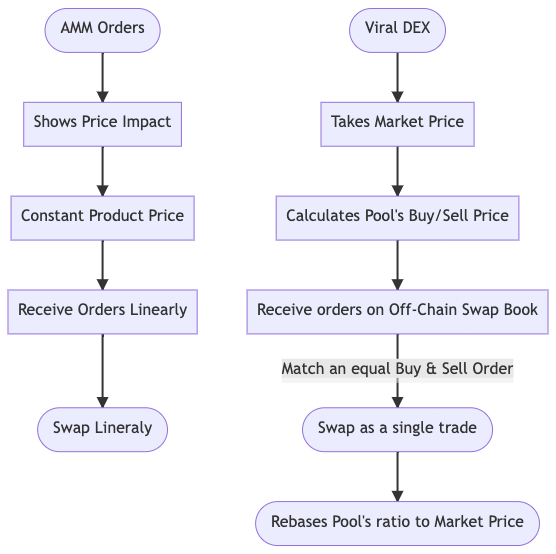
\includegraphics[width=7cm]{dex}
\caption{AMMs vs Viral DEX}
\end{center}
\end{figure}

\begin{comment}%mermaid
graph TD


    A([AMM Orders])
    C[Shows Price Impact]
    Z[Constant Product Price]
    D[Receive Orders Linearly]
    E([Swap Lineraly])

    A-->C-->Z-->D-->E
    F([Viral DEX])
    G[Takes Market Price]
    H[Calculates Pool's Buy/Sell Price]
    I[Receive orders on Off-Chain Swap Book]
    K([Swap as a single trade ])
    L([Rebases Pool's ratio to Market Price])

    F-->G-->H-->I--Match an equal Buy & Sell Order -->K-->L

    

\end{comment}

\textbf{Intro to Viral DEX}\\

Viral DEX is a Liquidity Pool exchange that matches buyers and sellers through it's swap book on top of it's Liquidity Pools while automatically rebasing the pool to it's live market's price thereby minimizing price impacts and proving faster and scalable trades using its micro-pool architecture\\

\textbf{Swap Book}\\

An Off-Chain Swap book similar to an order matching book will match buyers (Buy Primary Coin) and sellers (Buy Secondary Coin) and commence orders to a liquidity pool to swap between tokens. This order book is maintained on top of a liquidity pool to reduce price impacts and give a fair price for each token swap near to market price. 

\begin{figure}[H]
\begin{center}
\begin{tabularx}{0.8\textwidth} { 
  | >{\centering\arraybackslash}X 
  | >{\centering\arraybackslash}X 
  | >{\centering\arraybackslash}X 
  | >{\centering\arraybackslash}X | }
 \hline
 \textbf{Sell B} & \textbf{Buy A} & \textbf{Sell A} & \textbf{Buy B}\\
 \hline
 48.929687  & 1  & 0.43  & 21.869531\\
  \hline
 19.571875  & 0.4  & 0.946  & 48.112968\\
  \hline
 63.608593  & 1.3  & 0.344  & 17.495625\\
  \hline
 0.978593  & 0.02  & 1  & 50.859375\\
   \hline
   \hline
 133.088748  & 2.72  & 2.72  & 138.337499\\
\hline
\end{tabularx}
\caption{An Example Swap Book}
\end{center}
\end{figure}

To read a swap book one must need to determine the primary (A) and secondary Token (B). The token which has more value (typically in dollars) is a primary token compared to the lesser value secondary token. The buyers of primary tokens and sellers of secondary tokens are collectively considered as \textbf{Buyers} and the sellers of primary tokens and buyers of secondary tokens are considered as \textbf{Sellers}.

\begin{figure}[H]
\begin{center}
\begin{tabularx}{0.8\textwidth} { 
  | >{\centering\arraybackslash}X 
  | >{\centering\arraybackslash}X 
  | >{\centering\arraybackslash}X 
  | >{\centering\arraybackslash}X | }
 \hline
 \textbf{Sell DAI} & \textbf{Buy ETH} & \textbf{Sell ETH} & \textbf{Buy DAI}\\
\hline
\end{tabularx}
\caption{Example of an ETH/DAI Pool}
\end{center}
\end{figure}

Swap books contains prices derived from liquidity pool's current price and the trading pair's market prices. These continuous swaps determine the execution of orders into the liquidity pool and rebases the current liquidity pool's price to market price.\\

\textbf{Pricing Strategy}\\

In AMMs prices of swaps determined by the constant product formula $x \times  y=k$ where to swap $x$ tokens the liquidity pool will simulate the pool's after trade liquidity and by maintaining the $k$ constant it determines the amount of $y$ tokens a trader must provide. Whereas, in Viral DEX the constant product formula isn't used. Viral's Liquidity Pool execution of providing pool's liquidity will always require two simultaneous buy and sell of tokens with an addition of extra tokens to change the current price of pool to market price.

\begin{figure}[H]
\begin{center}
\caption{AMMs vs Viral DEX Swap match}
\end{center}
\end{figure}

\begin{center}
$Current\:Price\:of\:A = \frac{B}{A}$
\end{center}

A Pool's current price is determined by the ratio of the total tokens in the liquidity Pool. Since the current price isn't derived exactly from the market price, it might vary. Usual AMMs doesn't promises buy and selling of tokens in market rates, rather it is manually rebased to current market prices by arbitrage traders. Viral DEX doesn't provides the current buy price and sell price by calculating the ratio, rather it calculates the difference between the current market price and the current pool price and determines the buy and sell prices with conditions that can make the pool rebase to it's market price automatically when trades execute.\\

The Buy and Sell Price will always in regards to the market price because of the Viral's constant rebasing mechanism. The difference of market and current price is calculated by subtracting both prices. For Example in a ETH/DAI pool of ratio 5:2000 the current price is $\frac{B}{A}=\frac{2000}{5}=400$ where if the market price rose to 402 then the difference would be $Market\:Price - Current\:Price=402-400=2$

\begin{equation}
Difference\:D = Market\:Price - Current\:Price
\end{equation}

Thus a difference is taken into account to determine the buying and selling price of the current pair to rebase the price. The buy and sell price is determined by whether the difference is positive or negative. During bull market the difference will come in a positive integer when the $M.P>C.P$ market price is more than current price. Here the buy price of primary token will be added with the difference, where the sell price is the current price. During bear market the difference will come in a negeative integer when the $M.P<C.P$ market price is lesser than current price. Here the buy price of primary token will be the current price, where the sell price will be calculated by subtracting the difference\\

If D = positive $+$
\begin{equation}
Buy\:A=Current\:Price+Difference
\end{equation}
\begin{equation}
Sell\:A=Current\:Price
\end{equation}
If D = negative $-$
\begin{equation}
Buy\:A=Current\:Price
\end{equation}
\begin{equation}
Sell\:A=Current\:Price-Difference
\end{equation}

\textbf{Example Problem}\\

To understand how prices are calculated let's take an example problem. Find the pool's current price, buy \& sell price and difference while it's market price is less than 5\% of it's current price\\

\textit{Given} : Pool = 256/12526\\

\textit{Solution}\\
Here C.P = Current Price , M.P = Market Price\\
Given A = 256 , B = 12526 ;
To find current price 
\begin{equation}
C.P\:of\:A=\frac{B}{A}=\frac{12526}{256}=\frac{48.9296875}{1}=\frac{B}{A}
\end{equation}
Currently 1A=48.9296875B\\

Find M.P by subtracting 5\% of C.P $48.9296875 - ((48.9296875)(5\%))$ \\
\begin{equation}
M.P = 46.483203125
\end{equation}

Now, Find Difference between C.P and M.P $Difference\:D = Market\:Price - Current\:Price$
\begin{equation}
Difference\:D = -2.446484375
\end{equation}
If D = negative , $Buy\:A=Current\:Price$, $Sell\:A=Current\:Price-Difference$
\begin{equation}
Buy\:A = 48.9296875
\end{equation}
\begin{equation}
Sell\:A = 51.376171875
\end{equation}

\textit{Proof}
\begin{equation}
Final\:Price=\frac{C.P+Buy\:Price - Sell\:Price}{A} = 46.483203125
\end{equation}\\

Taking (7) \& (11) : $M.P=F.P$ Hence the buy and sell price is found and proved to move the token price to the market price. Similarly when the D (Difference) is positive the outcome will be achieved. \\


\textbf{Conditions and Requirements}\\

In centralized Order Books buyers are matched with sellers on the same price rate where in a swap book an order is executed when the sum of all buyers amount (Buy A or Buy B) should equal sum of all sellers amount (Sell A or Sell B) regardless of which token it is. This is a condition in a swap book for it to execute the order to a Liquidity Pool. Off-Chain Trading engines shall match summations of both buy \& sell amounts randomly and execute order and send funds to the users.\\

\begin{equation}
\sum_{n}^{\infty} BA_n = \sum_{n}^{\infty} SA_n
\end{equation}
\begin{center}
(or)
\end{center}
\begin{equation}
\sum_{n}^{\infty} BB_n = \sum_{n}^{\infty} SB_n
\end{equation}\\

In Equation (12) \& (13) the final index of the summations $\infty$ represents the limit of total number of table rows in the swap book e.g., $BA_1$ represents 1st row and Buy A column. The initial index $n$ indicates the swap book tables rows serial numbers where it's numbers are taken i.e., the swap amounts. The Summation term $BA_n, SA_n, BB_n, SB_n$ represents the addition of values taken from the tables. Here the Equation (12) constitutes that the summation of BA should be equal to summation SA and vice versa to be able to execute the swap. Where Equation (13) constitutes that the summation of BB should be equal to summation SB and vice versa to be able to execute the swap.\\

\textit{Example Swap Order}\\

A swap order in a Pool ratio of 256:1256 where it satisfies equation (12) to commence an order to the liquidity pool
\begin{center}
A = 256, B= 12526, C.P = 48.9296875, M.P=47,\\
D=-1.9296875, Buy 1 A=48.9296875 B , Sell 1 A=50.859375 B
\end{center}
\begin{figure}[H]
\begin{center}
\begin{tabularx}{0.8\textwidth} { 
  | >{\centering\arraybackslash}X 
  | >{\centering\arraybackslash}X 
  | >{\centering\arraybackslash}X 
  | >{\centering\arraybackslash}X 
  | >{\centering\arraybackslash}X | }
 \hline
 \textbf{Sl.no} & \textbf{Sell B (SB)} & \textbf{Buy A (BA)} & \textbf{Sell A (SA)} & \textbf{Buy B (BB)}\\
 \hline
 1 & 48.929687  & 1  & 0.43  & 21.869531\\
  \hline
 2 & 19.571875  & 0.4  & 0.946  & 48.112968\\
  \hline
 3 & 63.608593  & 1.3  & 0.344  & 17.495625\\
  \hline
 4 & 0.978593  & 0.02  & 1  & 50.859375\\
   \hline
   \hline
 Total & 133.088748  & 2.72  & 2.72  & 138.337499\\
\hline
\end{tabularx}
\caption{Example Swap Book matched order for $\sum_{n}^{\infty} BA_n = \sum_{n}^{\infty} SA_n$}
\end{center}
\end{figure}

\begin{equation}
Final\:Price=\frac{B+\sum SB - \sum BB}{A} = \frac{12526+133.088748-138.337499}{256}= 48.9091845664
\end{equation}\\

Here the total $\sum BA = \sum SA$ $2.72=2.72$ executes the order and changes the current price of 48.9296875 to  a final price of 48.9091845664 (Eq 14). After this trade the buy and sell price will be changed according to the difference $D=-1.9091845664$ Buy 1A=48.9091845664 and Sell 1A=50.8183691328 to bring the M.P to 47. Until the M.P is achieved the buy and sell price will change after each order execution.\\

Swap book order that satisfies equation (13) to commence an order to the liquidity pool\\
\begin{center}
A = 256, B= 12526, C.P of B = 0.02043749, M.P=0.015,\\
D=-0.00543749, Buy 1 B=0.02043749 A , Sell 1 B=0.02587498 A
\end{center}
\begin{figure}[H]
\begin{center}
\begin{tabularx}{0.8\textwidth} { 
  | >{\centering\arraybackslash}X 
  | >{\centering\arraybackslash}X 
  | >{\centering\arraybackslash}X 
  | >{\centering\arraybackslash}X | }
 \hline
 \textbf{Sell B (SB)} & \textbf{Buy A (BA)} & \textbf{Sell A (SA)} & \textbf{Buy B (BB)}\\
 \hline
 3297.339273  & 85.3185877421  & 39.0858162828  & 1912.45677834\\
  \hline
 2110.29713472  & 54.6038961549  & 47.172536893  & 2308.1374911\\
  \hline
 1187.04213828  & 30.7146915872  & 48.5203236614  & 2374.08427656\\
   \hline
   \hline
 6594.678546  & 170.637175484  & 134.778676837  & 6594.678546\\
\hline
\end{tabularx}
\caption{Example Swap Book matched order for $\sum_{n}^{\infty} BB_n = \sum_{n}^{\infty} SB_n$}
\end{center}
\end{figure}
\begin{equation}
Final\:Price=\frac{A+\sum BA - \sum SB}{B} = \frac{256+134.778676837+170.637175484}{12526}= 0.017574764
\end{equation}\\

Here the total $\sum SB = \sum BB$ $6594.678546=6594.678546$ executes the order and changes the current price of 0.02043749 to  a final price of 0.0175747644 (Eq 15). After this trade the buy and sell price will be changed according to the difference $D=-0.0025747644$ Buy 1B=0.0175747644 A and Sell 1B=0.0201495288 A to bring the M.P to 0.015. Until the M.P is achieved the buy and sell price will change after each order execution.\\

\textbf{Liquidity Limits for Rebase}\\

Using Viral DEX's pricing strategy for buying and selling by adding a difference $D$ rebasing, a necessary condition is needed to change the pool's current price to market price. The Total liquidity should be equal to the swap orders total volume i.e., In a 200/100 pool the sum of either buy or sell should attain it's pool's liquidity limit of 200 and 100 Tokens to change the pool to market price. While smaller pools rebases quickly, larger pools usually takes more time to get matched swap orders. To counter this liquidity and swap order issue the concept of Micro-Pools, Time Average Market Price (TAMP), Reserve Pools, Automated Pool Finding Algorithm are implemented.\\

\textbf{Micro Pool Architecture}\\

Viral DEX Pools implies a micro pool architecture for it's unlimited scalability and high throughput on swap orders. Since the protocol implies a swap book which will be matching total buys and total sells, the orders may get delayed in bigger pools which will require higher amounts of matches. Sharding the pools may increase the likeliness of getting matched and execution of users orders on the swap book. \\

Pools are sharded in percentages where the last added micro pool will be divided equally in to two parts $\frac{X}{2}$. This sharding will commence everytime a new blockchain is added to the Viral Smart Chain's -DEX Chains. Pool creators can able to shard their pools into existing number of DEX blockchains.


\begin{figure}[H]
\begin{center}
\begin{forest}
  forked edges,
  for tree={edge+={-Latex}},
  [100\%
    [50\%
		[50\%
			[50\%
				[50\%
					[50\%]				
				]				
				]		
		]    
    ]
    [50\%
    	[25\%
			[25\%
				[25\%
					[25\%]				
				]			
			]    	
    	]
    	[25\%
			[12.5\%
				[12.5\%
					[12.5\%]
				]
			]
			[12.5\%
				[6.25\%
					[6.25\%]				
				]
				[6.25\%
					[3.125\%]
					[3.125\%]				
				]			
			]    	
    	]
    ]
  ]
\end{forest}
\caption{Pool Shards after each new DEX blockchain addition}
\end{center}
\end{figure}

Each Micro-Pool determines each DEX blockchain added to the Viral Smart Chains where smaller pools can get increased volume in smaller transactions. When trade amount is lower the swap book will place the orders in smaller pools which may get matched faster whereas larger trades may get placed in larger pools or the trades will be divided among several pools to get matched and execute the swap successfully \\


The pools are represented in tables with rows mentioning number of pools where each pool will run on different blockchains and columns are represented to determine the cell value and percentage. Here $C_{11}, C_{22}, C_{33}, C_{44}.....C_{rc}$ are the pools that will be separated into two divisions equally ($50\%+50\%$) to form the new pool\\


\begin{figure}[H]
\begin{center}
\begin{tabularx}{1\textwidth} { 
  | >{\centering\arraybackslash}X 
  | >{\centering\arraybackslash}X 
  | >{\centering\arraybackslash}X 
  | >{\centering\arraybackslash}X 
  | >{\centering\arraybackslash}X
  | >{\centering\arraybackslash}X
  | >{\centering\arraybackslash}X
  | >{\centering\arraybackslash}X 
  | >{\centering\arraybackslash}X | }
 \hline
 \textbf{Chains} & \textbf{1} & \textbf{2} & \textbf{3} & \textbf{4} & \textbf{5} & \textbf{6} & \textbf{7} & \textbf{8}\\
 \hline
 \textbf{1}  & 100\% & & & & & & & \\
  \hline
 \textbf{2} & 50\%   & 50\%  & & & & & & \\
  \hline
 \textbf{3} & 50\%   & 25\%  & 25\%  & & & & & \\
   \hline
 \textbf{4} & 50\%   & 25\%  & 12.5\%  & 12.5\%  &  &  & & \\
    \hline
 \textbf{5} & 50\%   & 25\%  & 12.5\%  & 6.25\%  & 6.25\%  & & & \\
     \hline
 \textbf{7} & 50\%   & 25\%  & 12.5\%  & 6.25\%  & 3.125\%  & 3.125\%  & & \\
     \hline
 \textbf{8} & 50\%   & 25\%  & 12.5\%  & 6.25\%  & 3.125\%  & 1.5625\%  & 1.5625\%  & \\
      \hline
 \textbf{9} & 50\%   & 25\%  & 12.5\%  & 6.25\%  & 3.125\%  & 1.5625\%  & 0.78125\% & 0.78125\% \\
\hline
\end{tabularx}
\caption{Micro-Pool Table}
\end{center}
\end{figure}

\textbf{TAMP - Time Average Market Price}\\

As discussed in the earlier paragraphs the rebases successfully happen only if the trading volume equals the pool's total liquidity. This places a limitation of slower rebases due to the massive segregation of price impacts to every trader who wishes to buy/sell on the trading pair until the total trades rebases. To solve this limitation the concept of Micro-pools and Time Average Market Prices are introduced to traders. Micro-Pools fortunately split up the pools to rebase the smaller pools at first for the retail traders, where the smaller pools will rebase swiftly in real-time than larger pools. To benefit the large pool traders and to eliminate the real-time volatility during constant changes in rebase prices Time Average Market Price (TAMP) is brought out.\\

Each sharded pool will have different market prices derived from real time and delayed market prices in a following time period. Each sharded pool will have a time period configuration which will be determined by the number of DEX chains. For the first sharded pool $50\% + 50\%$ the time period will start with $2 seconds + 2 seconds$ where the market price shall be reflected every 2 seconds and calculated the buy and sell price of the current pool. Since most of the swap orders are instant swaps other than limit orders used by advanced traders, the buy and sell price of the pool will not affect the retail traders which changes every time period specified (in the example 2 seconds) regardless of pending swap orders left in the swap book.\\

Every Pool will have strict time period after which it can able to fetch the market price and update the buy/sell price. For Example., In 5 total sharded pools if Pool 5 has a time period of 16 seconds, the market price will be fetched every 16 seconds once and the buy/sell price will be altered according to the difference in the market and the pool's price. In short, according to the time period the market price is fetched from a decentralized oracle and will be used to determine buy/sell price for rebasing the pool. \\



\begin{figure}[H]
\begin{center}
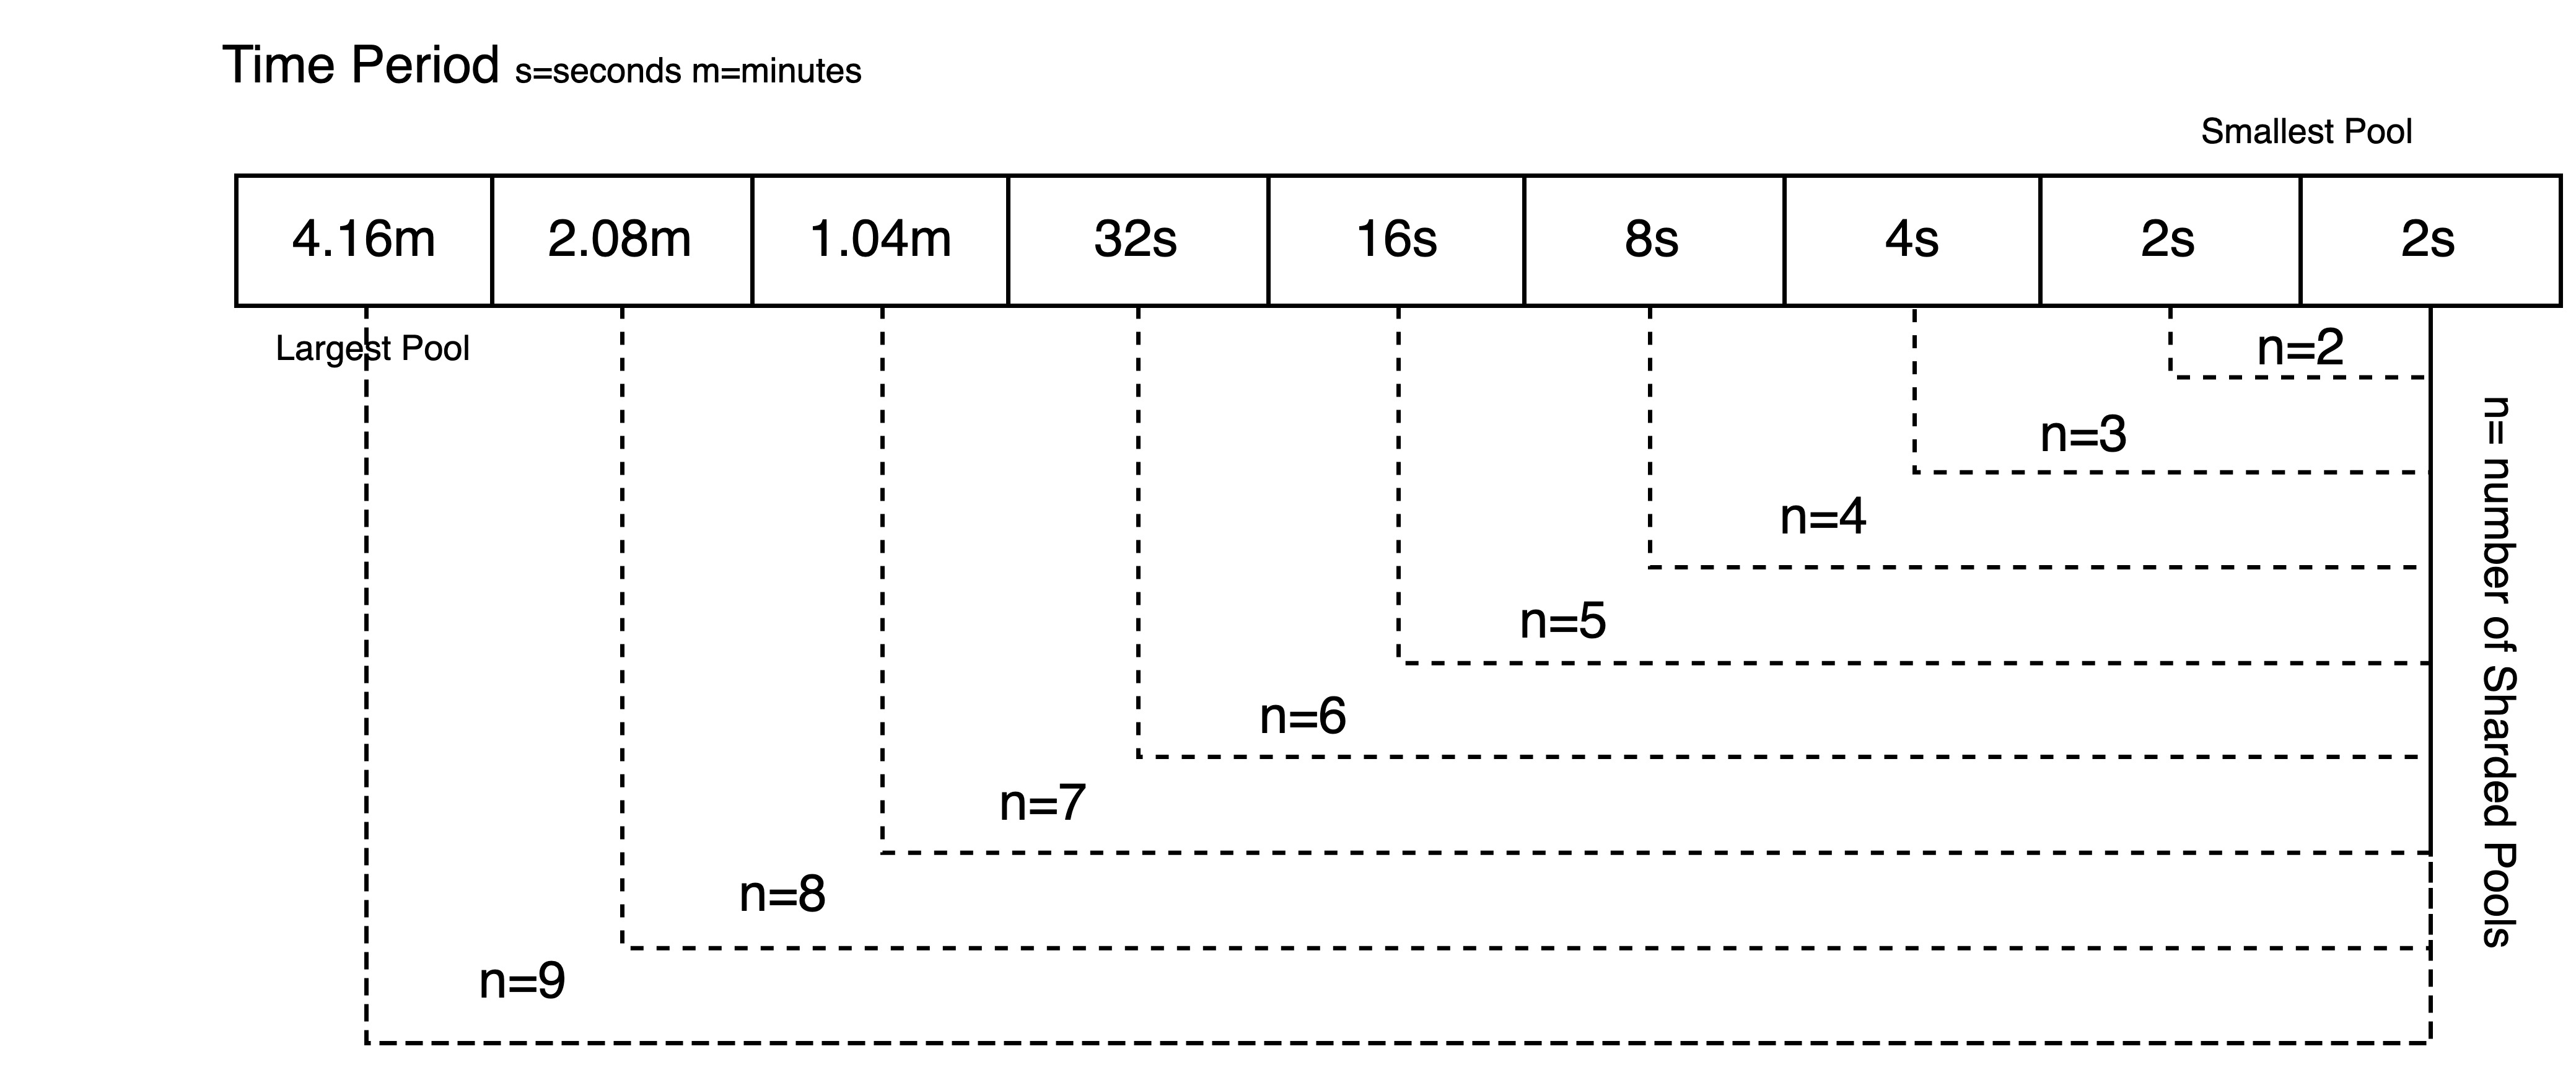
\includegraphics[width=\textwidth]{timeperiod-pools}
\caption{Time-period of Sharded Pools}
\end{center}
\end{figure}

For every new pool creation, the time period of all the pools will be updated accordingly. The time-period will increase by 2 times on the larger pool in descending order after every new pool is sharded i.e., 2,4,8,16,32,64,128,..n. 

\begin{figure}[H]
\begin{center}
\begin{forest}
  forked edges,
  for tree={edge+={-Latex}},
  [5 Total Pools
  	[Pool 1[50\%[16 sec]]]
  	[Pool 2[25\%[8 sec]]]
  	[Pool 3[12.5\%[4 sec]]]
  	[Pool 4[6.25\%[1 sec]]]
  	[Pool 5[6.25\%[1 sec]]]
  ]
\end{forest}
\caption{Example of Time-period of pools if number of pools (n) = 5}
\end{center}
\end{figure}

\textbf{Automated Pool Finding Algorithm}\\

Traders typically use DEX agregator softwares and applications to run complex mathematical algorithms across various DEXs to find the best possible price for a token swap with minimum impact. Most of the DEX employs a single pool for a given trading pair, where multiple DEX will have multiple pools of different algorithms and prices with price impacts. Viral implies a sharded multi-pool architecture where every pool will be priced to rebase according to the market price where the pools will have different prices. Due to the difference in prices users can able to make use of arbitrage trading by buying at low price pools or selling at higher price pools thereby running the protocol to rebase the pool by itself. \\

There are various factors a user can opt to get the best price possible. A trader can opt for two models of dex aggregator service provided in the Viral DEX, 1. Automated 2. Manual. In an automated service an algorithm is run to provide the best possible price by finding the perfect pool with the best price and instant swap support. Automated algorithm will be much faster than manual selection since it implies high efficient off-chain pool finder algorithm and can reduce man work. The user can opt for a manual method of selecting a specific pool according to his/her preference\\

\begin{figure}[H]
\begin{center}
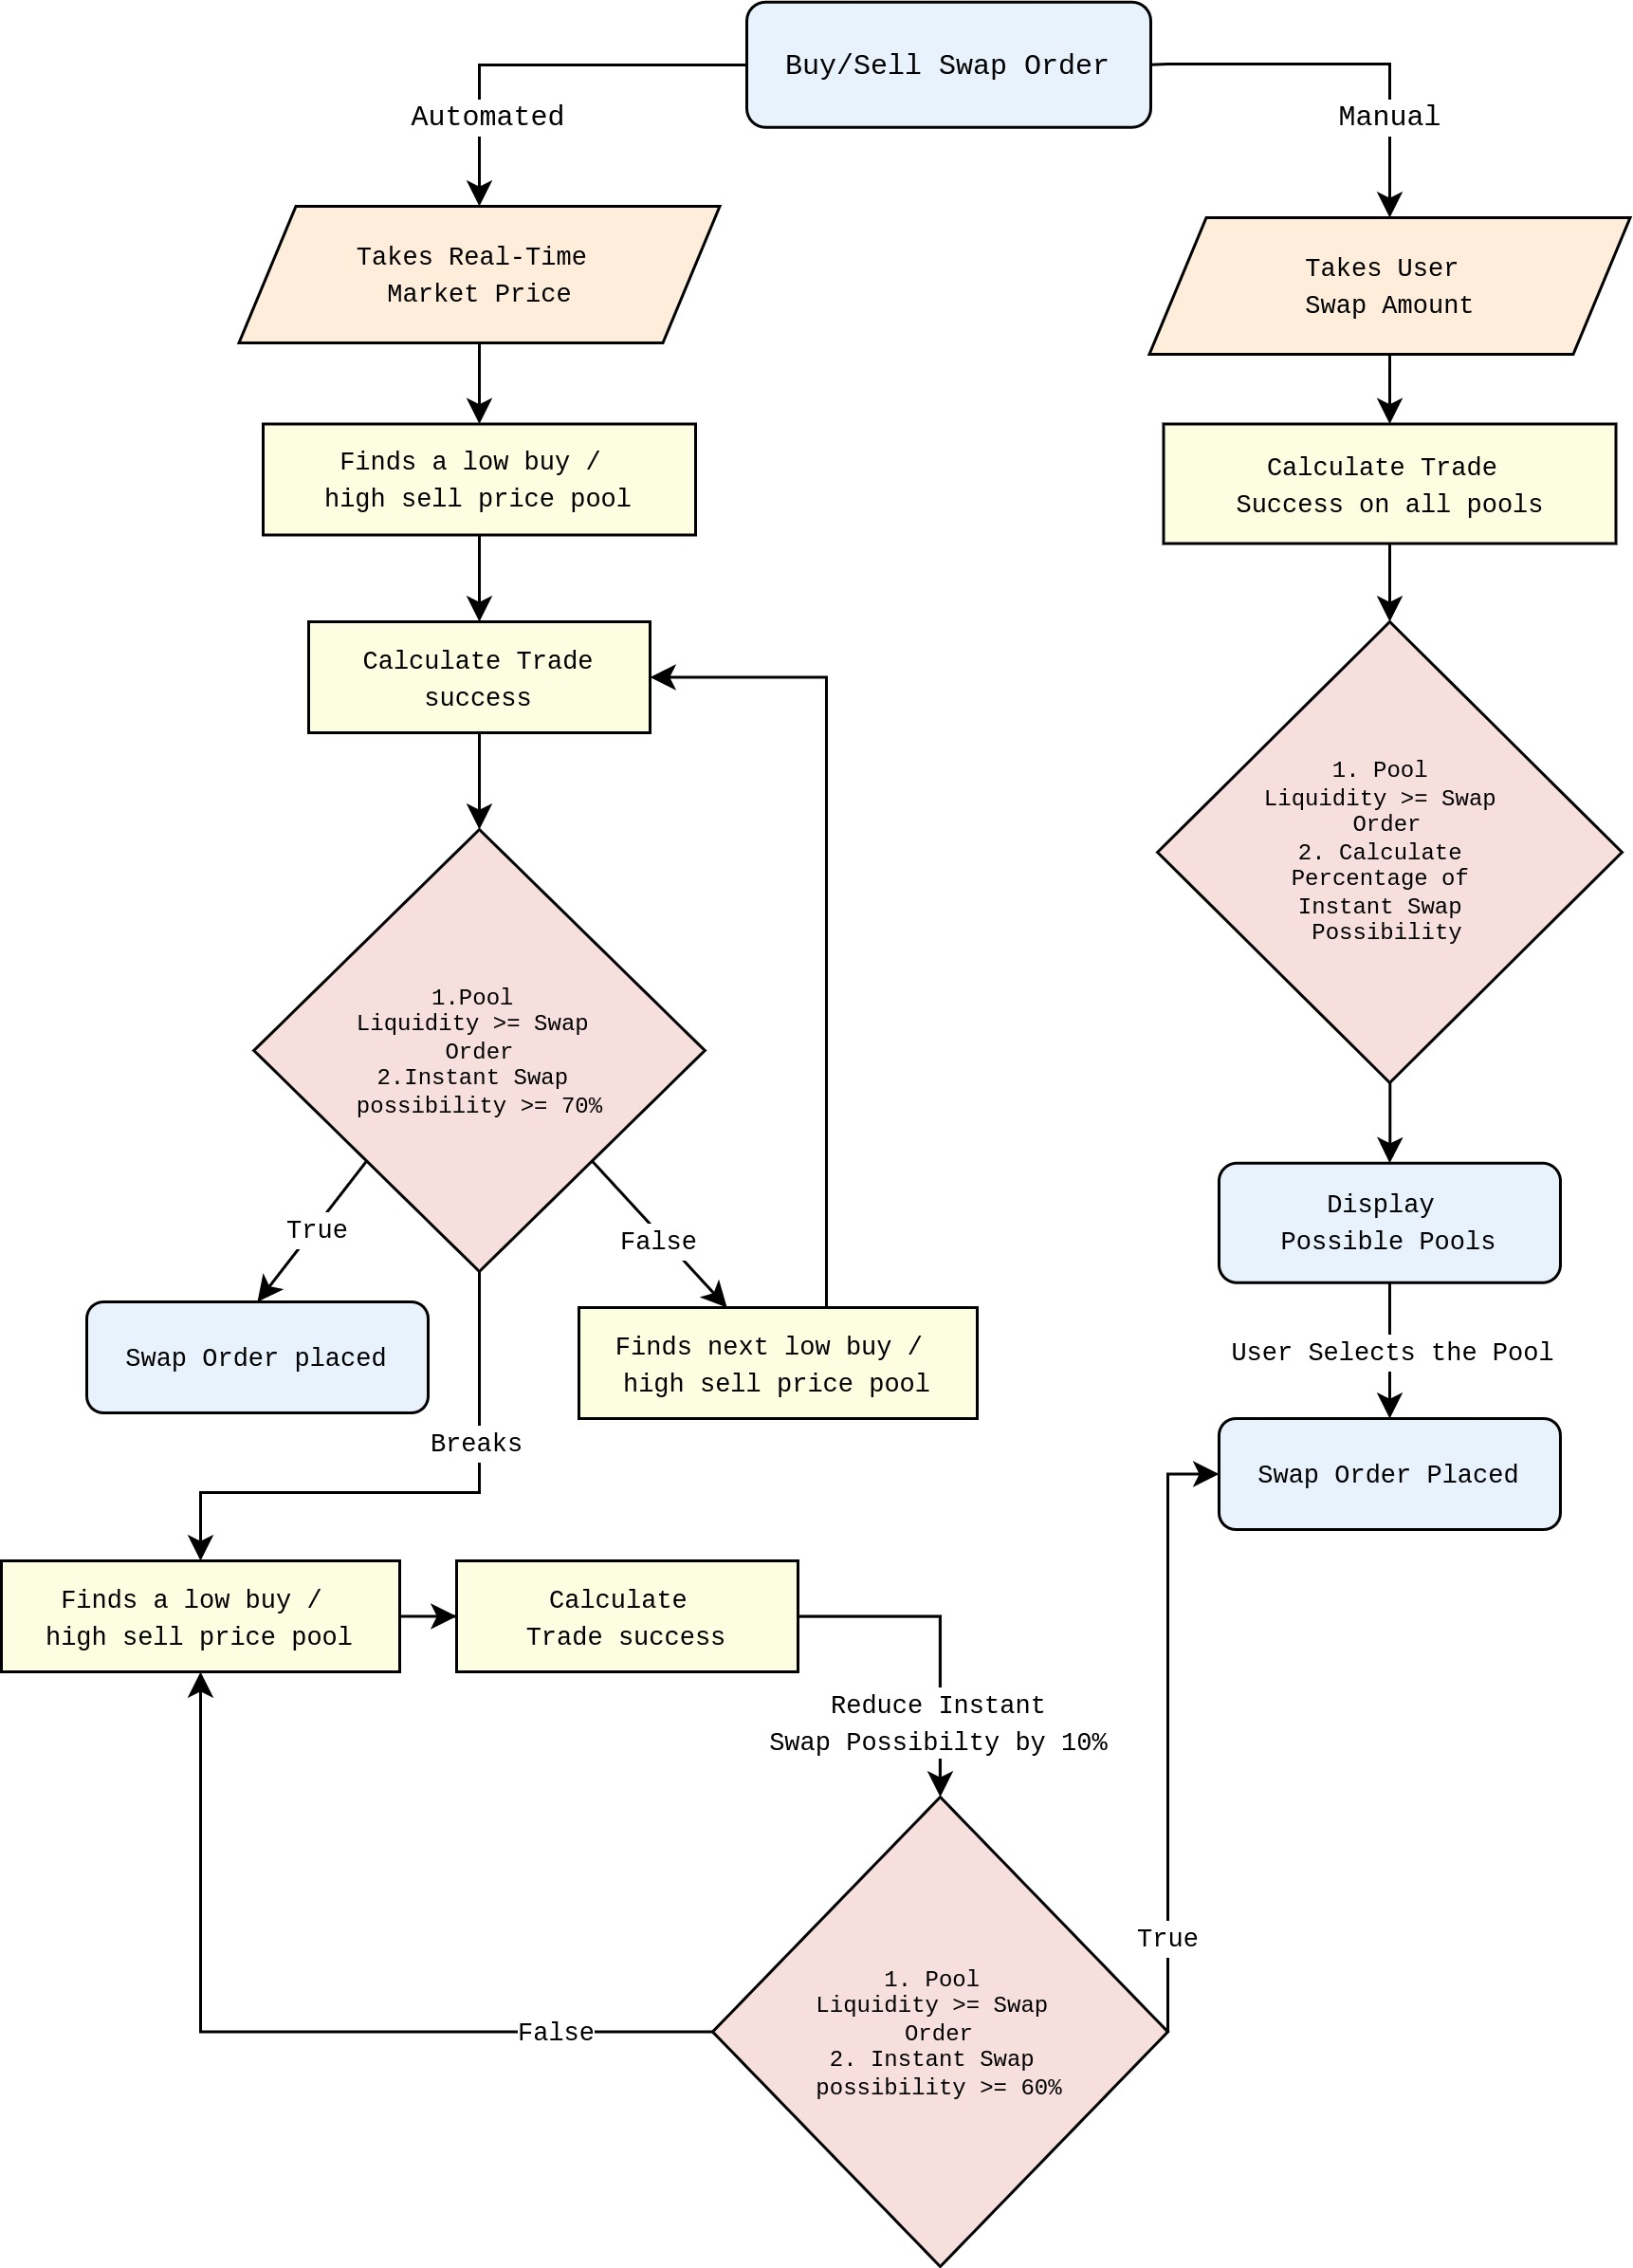
\includegraphics[width=11cm]{dex-algorithm}
\caption{Automated Algorithm for better price among swap orders}
\end{center}
\end{figure}

The algorithm run as follows,
\begin{itemize}[leftmargin=+0.2in]
\item Buyers always look for lowest price and sellers always look to sell for a higher price. The algorithm will work on finding the best low/high price for buy/sell.
\item The user/trader can opt for automated or manual method for a distributed or concentrated swap order
\item The Real Time Market Price and the Swap Amount is fetched to find the low buy/ high sell price pools for maximum benefits to the traders
\item The Swap on a particular pool can only be done if the total liquidity of the pool is lesser than the swap amount. In short, the swap amount shall not exceed the total pool liquidity (since Viral implements sharded pools)
\item The instant swap possibility is calculated by analyzing the pending swap orders that can match with the oppposite orders to instantly swap the trader's order once it sent to the swap book
\item If the Instant Swap Possibility is more than 70\% on the determined pool the swap order is sent to the swap book instantly, if not the algorithm will run on the next best pool. If neither of the total available pools for a specific token is having the instant swap possibility more than 70\%, the algorithm runs again on the best pools by decreasing the percentage by 10\% i.e., 60\%, 50\%, 40\%,...
\item Executing a swap in a lower instant swap possibility pools may increase the time to sucessfully carry out a swap on the Viral DEX pools.
\item Smaller Pools may have higher instant swap possibility, but the prices reflected are realtime. Hence the prices are near to market prices offering straightforward pricing rather than low buy and high sell prices.
\end{itemize}
\begin{equation}
Swap\:Order \leq Pool\:Liquidity 
\end{equation}
The Swap Order should always be lesser than each of the sharded pools i.e., the bigger pool may receive bigger orders but will always be limited to the pool's total liquidity, a trader cannot place a 100A Token order if the pool has a total liquidity of 80A. Since Viral has sharded pools the total liquiidty of all the pools are not considered rather a single pool is considered, so the pool of the bigger pool is considered as the max i.e., the 50\% Pool.\\
\begin{equation}
Instant\:Swap\:Possibility \geq n = 60\%
\end{equation}
\begin{equation}
For\:Unsuccessful\:Rounds \rightarrow n-10\%
\end{equation}\\
The Instant Swap Possibility is determined by calculating the total pending swap orders in the particular sharded pool's swap book that can execute the newly created swap order by matching the summation of the total buy orders and sell orders. The automated pool finding algorithm will find the best pool by calculating the pool's instant swap possibility and chooses the best pool accordingly.\\

\textbf{Reserve Pools}\\

Usual DEXs employing the AMM Constant Product Maker formula requires higher liquidity in it's single bigger pools to minimize the price impacts whereas Viral DEX sharded pools requires equal liquidity to trading volume per sucessful rebase. So, a considerable liquidity per pool is better enough to rebase the pool's price to current market price of the token pairs. If a higher liquidity is provided to sharded pools where only a smaller liquidity is needed, the rebases get delayed making a spike in the price impact for the following traders making them to encounter a increased price slippage on their swap orders. Surplus of excess liquidity can be avoided in Viral DEX compared to current AMM Exchanges. Smaller sharded pools rebases much quickly in seconds where bigger pools takes couple minutes to fetch the market price and adjust the buy/sell price for the pool to rebase. To counter the effect of delayed rebases of sharded pools due to higher liquidity more than the stipulated trading volume per time period the concept of Reserve Pools are used.\\

Reserve Pools are smart contract accounts that is maintained by the trading pair's pool contract which freezes a certain portion of tokens from the liquidity pool to match the trading volume for rebasing the sharded-pools. It is exactly the same as withdrawing a certain percentage of liquidity but to a smart contract that holds the funds separately which accounts for decreasing the pool's liquidity for smoother rebases.\\

\begin{figure}[H]
\begin{center}
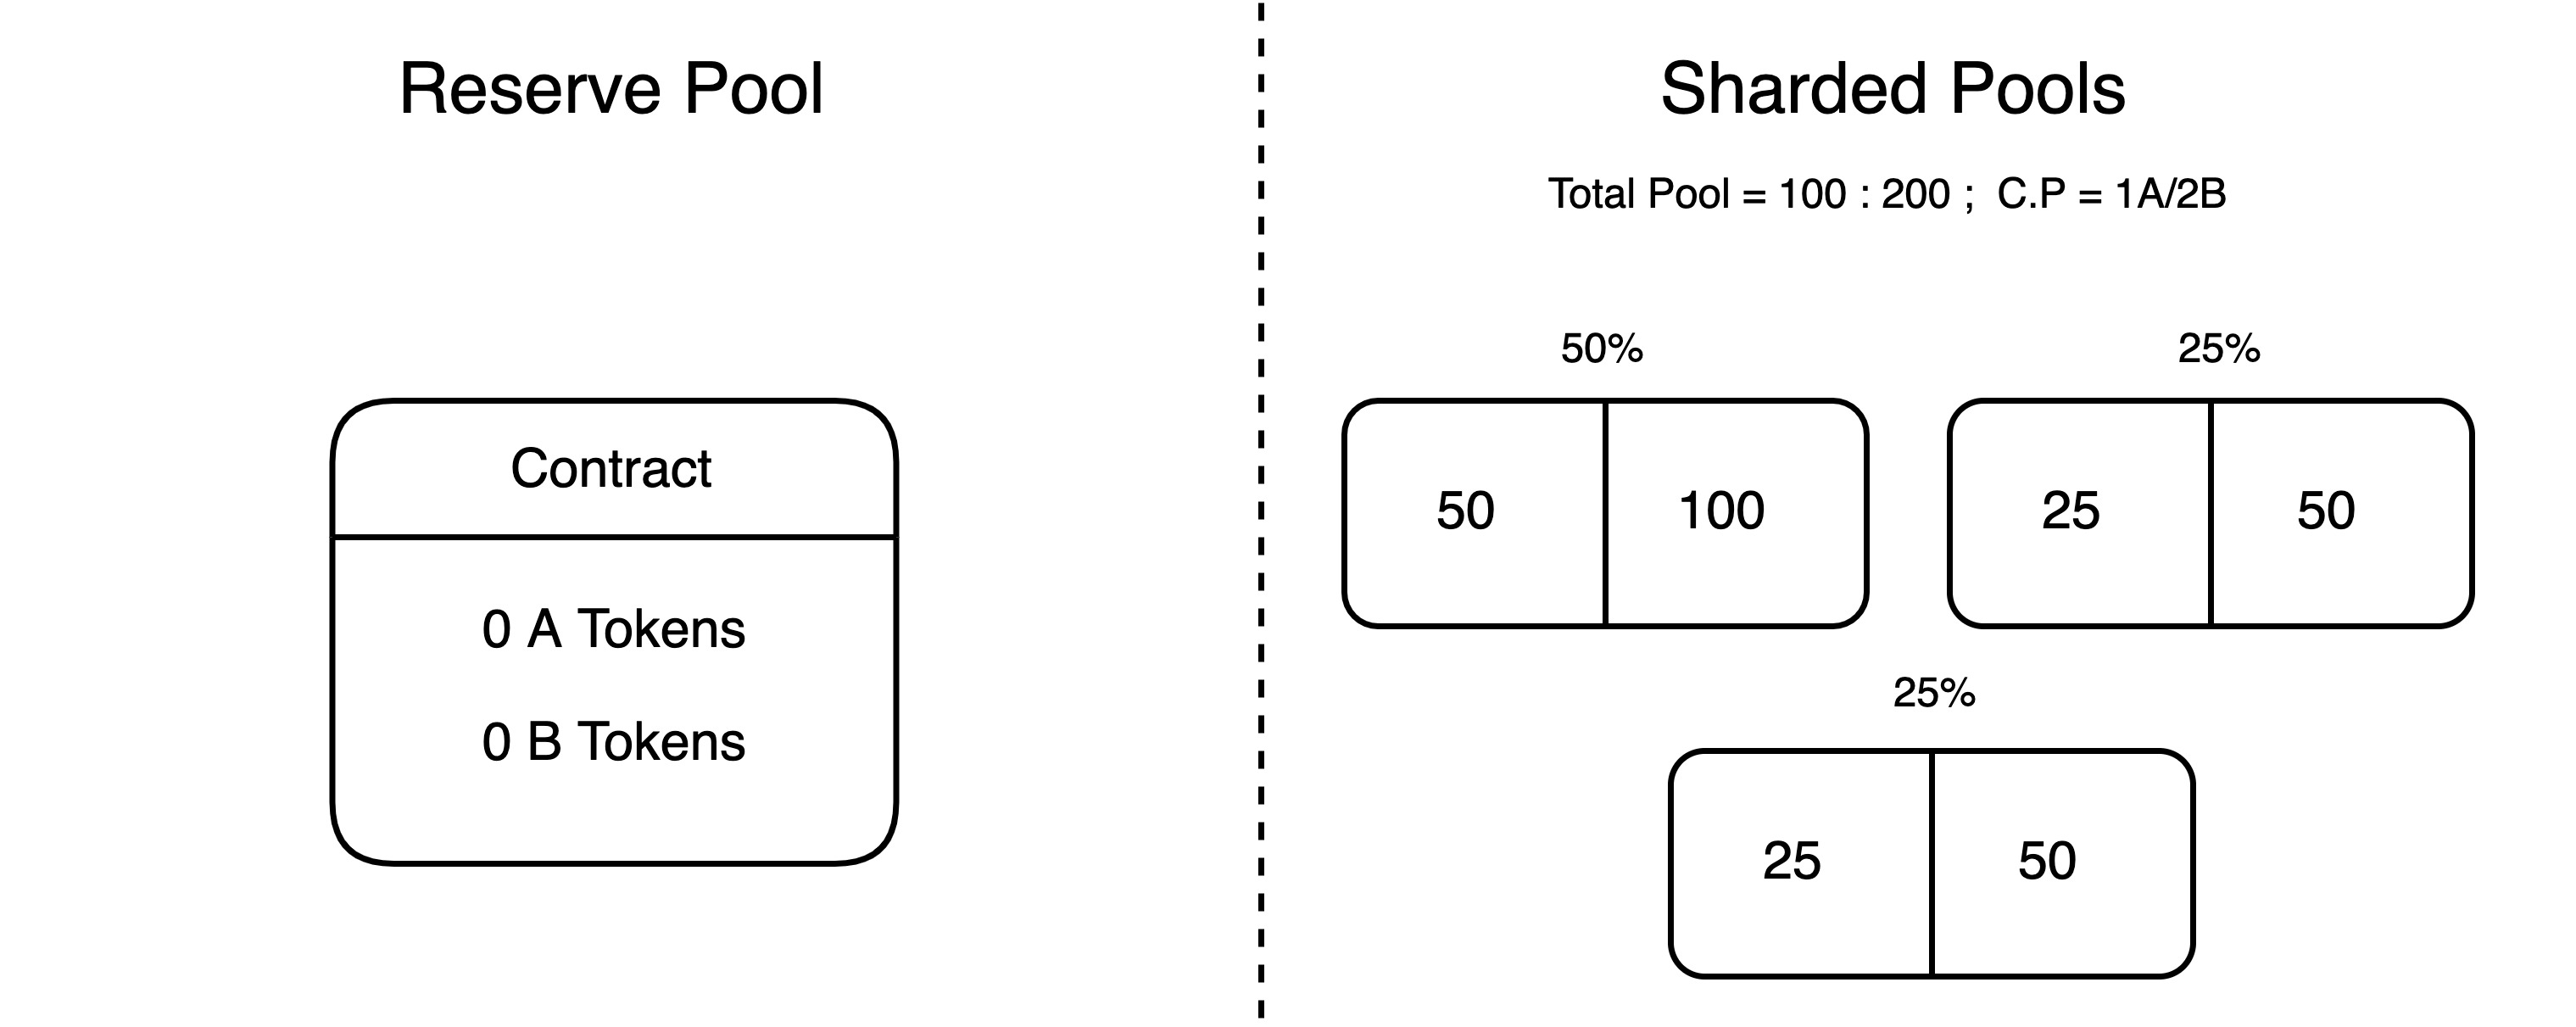
\includegraphics[width=13cm]{reserve-pool-1}
\caption{Initial Creation of Pools}
\end{center}
\end{figure}

During the initialization of the pool, the reserve pool will be set to zero where the pools will be sharded according to the pool creator's configuration where the number of dex-chains are the limit. The pools get sharded by percentage and the market price is been set by an oracle to fetch and provide buy and sell price according to the difference in current price of the pool and market price of the trading pair.

\begin{equation}
Limit Equation For Number Of Dex Chains = Pool Shards Configurations
\end{equation}

Liquidity gets freezed and sent to reserve pool on two occasions
\begin{enumerate}[leftmargin=+0.2in]
\item \textbf{Zero Trading Volume} : Some Pools are created for low-volume tokens that will receive low to no swap orders which then accounts for a huge price impact if the value suddenly sky-rockets making the pool to react differently to price impacts and delayed rebases
\item \textbf{Reduced Trading Volume} : Reduced trading volume gives pressure on delayed rebases on sharded pools which can be prevented by decreasing the liquidity in the pool by withdrawing it into a seperate reserve pool (similar to a wallet account but as a smart contract) 
\end{enumerate}

Pools will withdraw tokens in to its reserve pool on request. The withdrawal ratio will be equal to the Current Price ratio of the current pool not affecting the pool's price. When each pool has different ratio of tokens (possible scenario due to Time Average Market Prices- TAMP) an equal percentage from all the pools shall be withdrawn to maintain the micro-pool architecture. In simple words from each pools the tokens will be withdrawn at a same percentage and sent to it's reserve pool to decrease the liquidity for better rebases.\\


\textbf{Limit Orders}\\

Viral uses an off-chain swap book that matches the summation of primary coin/secondary coin buy and sell orders to execute a swap in the Viral DEX Liquidity Pools that sets a pricing strategy in accordance with rebasing the pool's liquidity to fetched real-time market price of the trading pair. Since it incorporates an off-chain swap book without executing the swap instantly like other DEXs the makers can benefit the features of limit orders and therby making the trading pair liquid in nature. Users can make use of limit orders to buy and sell when the maket reaches a certain price. The limit order gets placed in a seperate book that will run automated pool find algorithm and determines when a pool reaches a limit price and passes the order to the swap book and executes the swap instantly.\\


\textbf{Fee Structure}\\

Viral DEX subtracts a swap fee on every swap order executed. There are two types of fee leaved according to trading pairs nature. A 0.2\% fee will be leaved on normal pairs and a 0.02\% fee will be leaved for stable-coin pairs. These DEX fees are excluding wallet transfer fees which will be leaved separately. These fees will be added into a separate pool where the liquidity providers can collect while withdrawing their staked tokens. 70\% of total DEX fees collected with be allocated to liquidity providers where the rest 30\% will be sent to Viral's global revenue pool.\\

\begin{figure}[H]
\begin{center}
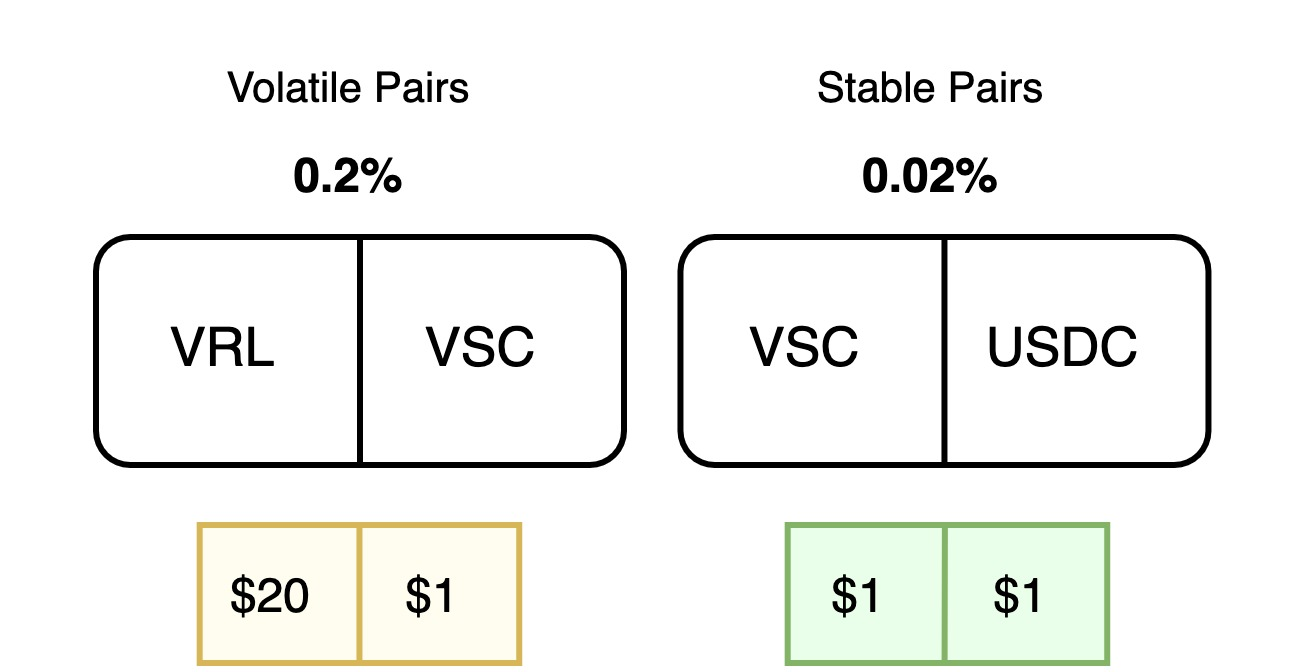
\includegraphics[width=9cm]{dex-fee}
\caption{Fee Structure}
\end{center}
\end{figure}

\begin{equation}
Normal\:Pair\:Swap\:Fee=Swap\:Amount \times  0.2\%
\end{equation}
\begin{equation}
Stable\:Pair\:Swap\:Fee=Swap\:Amount \times  0.02\%
\end{equation}
\begin{equation}
Transfer\:Fee=After\:Swap\:Fee\:Rate \times  Transfer\:Fee
\end{equation}\\

\textit{For Example} 
(Fee Type : Normal Pair) \\
Total Swap amount = $500$\\
DEX Fee : $500 \times  0.2\% = 1$ \\
Transfer Fee= $((500)-(500 \times  0.2\%)) \times  0.05\% = 0.2495$ \\
Final = $498.7505$\\

(Fee Type : Stable Pair) \\
Total Swap amount = $500$\\
DEX Fee : $500 \times  0.02\% = 0.1$ \\
Transfer Fee= $((500)-(500 \times  0.2\%)) \times  0.05\% = 0.24995$ \\
Final = $499.65005$\\
 
 
\textbf{Liquidity Providers}\\

Liquidity providers are investors who stake their cryptocurrency tokens on DEXs to earn transaction fees, often referred to as liquidity mining or market making. Viral Liquidity providers earn transaction fees for their staked tokens in the Viral Smart Chains protocol. The transaction fees are distributed proportionally to all the liquidity providers in the pool according to their percentage of investment. Sine Viral implies micro-pool architecture the liquidity is divided among several micro-pool running blockchains while depositing and withdrawing funds.\\


\textit{For Example}\\

Pool = 1600 : 4,992 LP provides tokens 20 : 62.4 equally to the pool. No.of Micro-Pools = 4\\

\begin{figure}[H]
\begin{center}
\begin{forest}
  forked edges,
  for tree={edge+={-Latex}},
  [20 : 62.4
    [50\%
        [10 : 31.2]
    ]
   [25\%
        [5 : 7.8]
    ]
    [12.5\%
        [2.5 : 3.9]
    ]
    [12.5\%
        [2.5 : 3.9]
    ]
  ]
\end{forest}
\caption{Division of LP funds to micro-pools}
\end{center}
\end{figure}

When an LP withdraws their funds it will be distributed according to his percentage of initial investment percentage i.e If a LP provide 10:20 in a 100:200 Pool, the LP holds 10\% of the pool's liquidity, after multiple trades and rebases the LP's funds might be proportionally distributed among the main pool, reserve pool and transaction fee pool, when the LP withdraws he shall receive the 10\% allocated. The Reserve pool can be determined as a wallet smart contract that hold's the LP funds which are not required for the main pool. When a small percentage of LP's invest their tokens into a restricted liquidity pool, thet trnsaction fee may distributed among a small group of LP's which can provide a better ROI compared to current AMM pools.


\begin{figure}[H]
\begin{center}
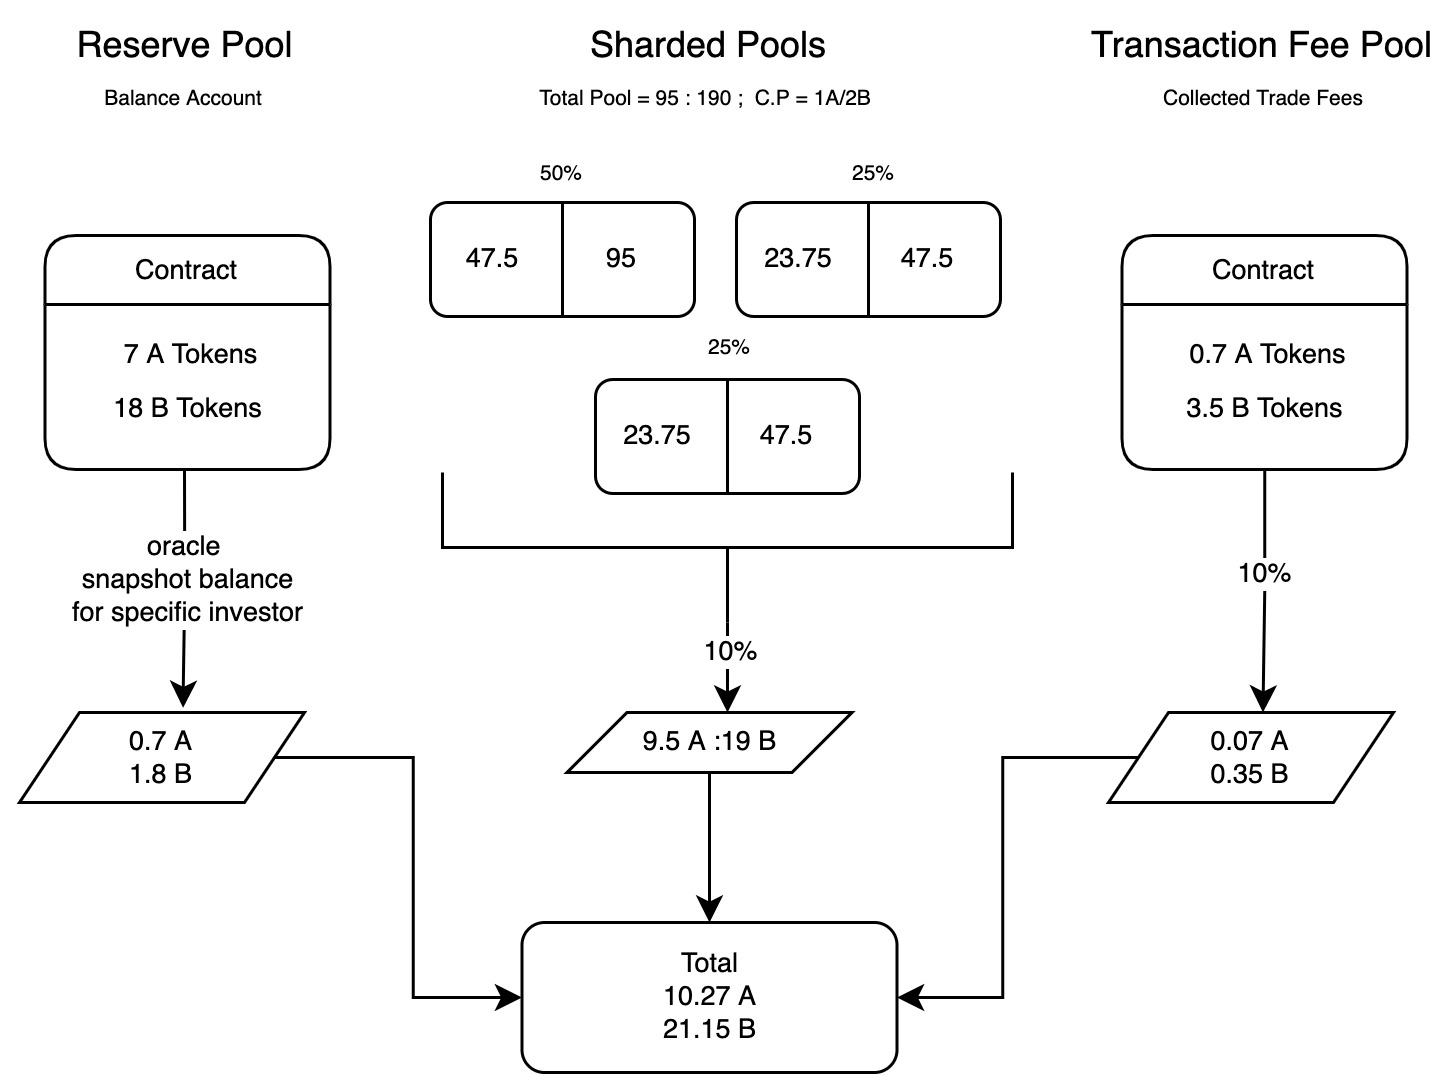
\includegraphics[width=13cm]{reserve-pool-4}
\caption{Liquidity Provider withdrawal of Funds from all reserves}
\end{center}
\end{figure}

\textbf{Benefits of Viral DEX}
\begin{enumerate}[leftmargin=+0.2in]
\item \textbf{Affordable Fees} : Competitive low-priced fees 0.2\% for Normal pairs and 0.02\% for Stable pairs.
\item \textbf{Free from Price Impacts} : Price impacts are eliminated since to execute a swap order both the buyer and seller orders should be matched and swapped at once as a single order which eliminates the price impacts.
\item \textbf{Real-Time Market Price Pool Rates} : Constant Product Maker is not used rather the pool will determine the buy \^ sell price by finding a difference between the current pool price by it's ratio and the market price of the trading pair to rebase the pool always to the market price.
\item \textbf{Faster Swaps} : Sharded Micro-pools deployed on separate chains brings parallel executions of faster swaps .
\item \textbf{Reduced Human-work} : Automated Pool Finding Algorithm shall find the best pool by determining the lowest buy / highest sell price and instant swap possibility by calculating how much liquid a particular pool's swap book orders are.
\item \textbf{Multi-Layer Security} : The Viral Multi-Chain Architecture  offers an immutable state anchoring of each chain's global state to the Tangle (DAG) for additional security.
\item \textbf{Advanced Trading} : Since Viral employs a strategy to receive all the orders on a off-chain swap book, it can receive limit orders for institutional and retail market makers who would like to trade on DEXs.
\item \textbf{Less Volatility} : Real-Time Market Prices are taken in account for the pool rebases that makes the pool less volatile compared to current AMMs that have huge volatility upon larger orders.
\item \textbf{Congestion-Free DEX} : Congestion is eliminated by incorporating micro-pools where larger pools for larger orders and smaller pools for smaller orders.
\item \textbf{Multi-Order Matching} : Comparing to Order book exchanges which matches a buyer and seller, where Viral DEX matches multiple orders who can execute an order in a single swap.
\item \textbf{Higher Yields for LPs} : Unlike current AMMs that require larger pools to become stable without volatile effects, Viral requires only a liited amount of Liquidity equal to the trading volume, which can provide a smaller group of LP's maximum yields.
\end{enumerate}

\subsection{Viral Fiat-Exchange}

Centralized exchanges (CEXs) are a type of cryptocurrency exchange that is operated by a company that owns it in a centralized manner. Centralized exchanges most commonly facilitate trades between users by maintaining an order book: a collection of buy and sell orders posted by individual traders. CEX users do not actually exchange crypto or fiat currencies with each other. Instead, when they deposit their funds onto an exchange, the latter takes over the custody of the crypto assets and issues a corresponding amount to the buyer and seller. Users store their crypto assets on the exchange. Since the private key's ownership rests with the exchange, there is a risk of total loss should the exchange be compromised (Not your Keys, not your Coins). Cases of this kind are rare but historically have already occurred with losses in millions. CEX exchanges are under the control of regulators, third-party providers, and legal regulations. To prevent money laundering, operators are required to collect extensive data about their customers (KYC). This regularity is contrary to the basic idea of cryptocurrencies.\\

\textbf{Common Insecurities Investors have on Centralized Exchanges}\\

Ironically, many of the same factors that contribute to the advantages of a centralized exchange also contribute to the disadvantages.
\begin{enumerate}[leftmargin=+0.2in]
\item \textbf{Custody}: Entrusting an exchange with your private keys means you don’t fully control your own money.

\item \textbf{Security}: Because they hold a large number of assets, centralized exchanges are a prime target for bad actors. The most notorious exchange hacks were aimed at centralized exchanges (e.g., Coincheck, Mt. Gox, BitGrail, NiceHash, and Bitfinex).

\item \textbf{Manipulation}: Several centralized exchanges have been accused of manipulating their opaque nature and conducting insider trading, fake volume, and price manipulation.
\end{enumerate}

\textbf{Security Threats}\\

As the security threats continues, there's currently no effective solution for a non-custodial fiat-crypto exchange. At any instance if a probable propaganda is proposed the primary user aquisition strategy of those solutions is to target the current users of popularly running cryptoexchanges which is a very long and narrow way to bring in users for the platform. Viral has a first mover advantage for such a non-custodial way of buying cryptocurrencies using fiat-currencies since it's application offers end to end solution on all aspects on the de-fi wave, user's are prompted to use it's services while using the application. This has a significance effect in acquiring users for an in-built crypto buying facility for users to trade in their fiat money. For one such of an exchange where it's users derived from a social media will impact the crypto adoption and also reassures the year-long threat of losing user's funds to potential hackers.\\

\textbf{Intro to Viral-FEX}\\

Decentralization refers to freedom and ownership. A centralized exchange restricts the ownership by being a custody to user's funds by maintaining the private keys on their central server. There is only two aspects a CEX will carry out: Buying and Selling. While both fiat and crypto funds is being held in custody, the Fiat Funds is securely holded (due to it's reversal mechanism), whereas the Crypto Funds are always open for attacks and cannot be reverted back nor easy to track the route of transactions to an individual after a breach. While Popular CEXs are tackling these breaches using secured cryptographic encryptions, firewalls, etc there is always a possibilty for a penetration expert to steal the funds. Viral is offering a non-custodial crypto buying solution by supplying fiat-pegged-tokens and exchanging via Viral DEX.\\

\textbf{Basic Structure}\\

Viral Buy/Sell Exchange works differently from centralized exchanges. In current CEXs when user deposits his fiat funds, the funds will get deposited into the exchange's traditional banking account from where the user gets his fiat balance updated with a total figure he would have deposited. CEXs tracks user's fiat balances in a centralized manner and directly updates the database tables of each user after making successful trades. The update in fiat balances are done through centralized systems which is not transparent and needs to be trusted. This effectively comes to the usage of Fiat-backed-crypto tokens such as USDC, USDT, TrueUSD which holds equally backed fiat amount in reserves and thereby minting new tokens for user in which the is pegged 1:1 to a government backed fiat currency .i.e., typically US Dollar.\\

Nowadays most users prefer to buy USDC and later use those tokens in various DeFi applications. The emergence of fiat backed tokens have paved a way of tokenizing fiat coins. As Viral's vision to bring rapid adoption to tokenized economy we provide our users to buy Viral Coins from fiat currencies by adopting fiat-tokenization strategy and swap books of Viral DEX for exchanging tokenized fiat to Viral Coin and vice versa.\\

In simple words while today's crypto exchanges updates the fiat balance when users deposit their fiat currencies i.e., dollar, euro, yen, rupee into the exchange, while Viral Exchange provides users who deposit an equivalent amount of special Fiat-Tagged tokens (Eg; USD, INR, EUR - all as crypto tokens) into their current non-custodial Viral wallet that can be referred as fiat balance from which users can trade in for Viral Coins. While buying and selling Viral Coins the users will be using their Fiat-Tagged Tokens to facilitate trades using a decentralized Swap Books Exchange between white-listed addresses\\

A solution which combines decentralized solutions is a better, safer and cheaper alternative to current custody model exchanges. Since deposit and withdrawal of fiat funds are subject to regulatory compliance some of the process such as KYC, AML will be required for users. Some of the benefits compared to current exchanges are
\begin{enumerate}[leftmargin=+0.2in]
\item \textbf{Security of Funds}: Stored in Non-Custodial Wallet
\item \textbf{Decentralized Exchange}: Atomic Swaps happen on-chain and orderbook will be maintained off-chain
\item \textbf{User Owned Private Key}: Hot Wallets where user owns his/her private key and has complete ownership of deposits
\end{enumerate}

\textbf{User Registration}\\

\begin{figure}[H]
\begin{center}
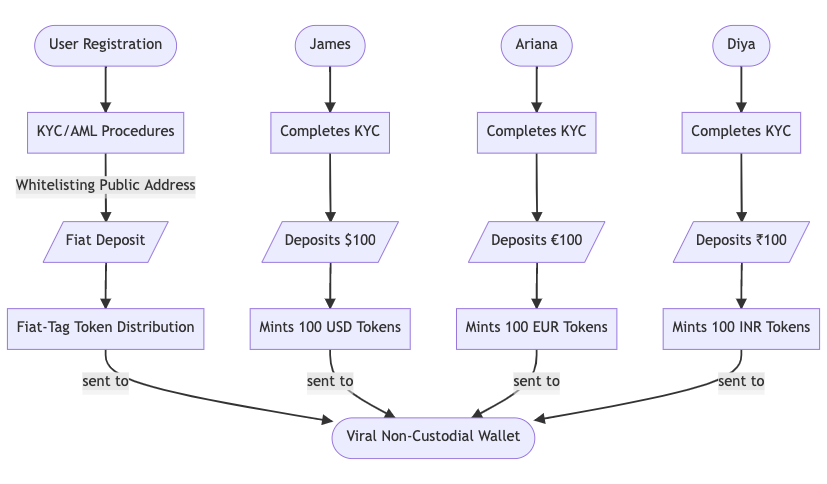
\includegraphics[width=10cm]{user-deposit}\\
\caption{User Deposit and Fiat-Tag Token Distribution}
\end{center}
\end{figure}


\begin{comment}%mermaid
graph TB
    
    A([User Registration])
    C[KYC/AML Procedures]
    D[/Fiat Deposit/]
    E[Fiat-Tag Token Distribution]
    A-->C--Whitelisting Public Address-->D-->E

    F([James])
    G[Completes KYC]
    J[/Deposits \$100/]
    K[Mints 100 USD Tokens]
    F-->G-->J-->K

    L([Ariana])
    M[Completes KYC]
    N[/"Deposits €100"/]
    O[Mints 100 EUR Tokens]
    L-->M-->N-->O

    Q([Diya])
    R[Completes KYC]
    S[/"Deposits ₹100"/]
    T[Mints 100 INR Tokens]
    Q-->R-->S-->T


    P([Viral Non-Custodial Wallet])
    E & K & O & T--sent to-->P
\end{comment}

While Viral application doesn't require any user information, ViralFEX will require user's information such as email, phone verification, etc and also will require Know-Your-Customer (KYC) and Anti-Money-laundering (AML) policies for regulatory purposes. After the registration completes the user's viral wallet username (VNS) will get linked automatically to get white-listed for the exchange (since it's decentralized) and securely drop in fiat-tag tokens directly into the user's VNS-linked Viral Smart Chain wallet address. 


\begin{figure}[H]
\begin{center}
\begin{forest}
  forked edges,
  for tree={edge+={-Latex}},
	[Fetches Viral Username
		[Whitelists-username
			[$username$ returns address $0x71C7656EC7ab88b098defB751B7401B5f6d8976F$]		
		]	
	]
\end{forest}
\end{center}
\end{figure}

\textbf{Fee Structure}\\

Since Viral-FEX deals with only deposit \& withdrawal where the exchanging mechanism depends on swap books and ViralDEX Pools the fees on  Viral Semi-CEX is considerably low compared to other popular centralized exchanges. Viral takes fees based on deposit, withdrawal and trade. These fees doesn't include the network fees paid to the Viral Smart Chain which will be included seperately. Since Viral Smart Chain doesn't take gas fees and takes a very minute amount of base fee \$0.0005 and a transfer fee of 0.05\% it will not affect the users trades. The exchange fees are listed below\\

\textbf{Deposit fees}
\begin{enumerate}[leftmargin=+0.2in]
\item \textbf{Deposit Fee}: Fized 0.1\% excluding credit/debit card or bank transfer fee
\item \textbf{Mint Fee}: Fee charged for minting new fiat-tag tokens .i.e., typically \$0.0005
\end{enumerate}

\textbf{Trade Fee}\\

The trade fee is fixed to 0.2\% for Viral Coin- Fiat Pairs and 0.02\% for Viral Stable Coin - Fiat Pairs. These fees will be allocated to 70\% Liquidity Providers and 30\% Viral Global Revenue Pool\\

\textbf{Withdrawal Fee}
\begin{enumerate}[leftmargin=+0.2in]
\item \textbf{Withdrawal Fee}: Fixed 0.1\% excluding credit/debit card or bank transfer fee
\item \textbf{Burn Fee}: Fee charged for burning fiat-tag tokens .i.e., typically \$0.0005
\end{enumerate}


\textbf{Fiat-Tag Token Supply}\\

Fiat-Tag Tokens are limited tokens that is minted and supplied to FEX users after depositing fiat money i.e., USD, EUR, INR, etc to their exchange accounts. The utility of these tokens is only limited for exchanging purposes inside the viral application. The tokens are classified by listed fiat currencies from which users are allowed to exchange e.g., If Euro can be deposited to Viral FEX account, EUR Tokens will be generated and sent. The supply of tokens are elastic in nature while minting and burning while depositing and withdrawing fiat funds. KYC users addresses will be white-listed for transacting fiat-tag tokens to eliminate spam and usage of tokens by a non-kyc users.\\

\begin{figure}[H]
\begin{center}
\begin{tabular}{ |p{3cm}||p{3cm}|p{3cm}|p{3cm}|  }
 \hline
 \multicolumn{4}{|c|}{Fiat-Tag Tokens} \\
 \hline
 Fiat Currency & Fiat-Symbol & Region & Tag-Token\\
 \hline
 US Dollar &\$ & United States & USD\\
 Euro & €  & Europe  & EUR\\
 Japanese Yen &¥ & Japan & YEN\\
 Pound Sterling &£ & Britain & GBP\\
 South Korean Won &₩   & South Korea & KRW\\
 Indian Rupee &\rupee & India  & INR\\
 Canadian Dollar &\$ & Canada  & CAD\\
 \hline
\end{tabular}
\caption{ViralFEX Fiat Tag Tokens}
\end{center}
\end{figure}


\textbf{Minting Tag-Tokens / Fiat Deposit}\\

Fiat-Tag Tokens will be minted upon a KYC user's deposit of funds to allocated fiat-holding reserve bank. User's funds are holded by custodian banks fiat holding accounts. Viral allows partnership of centralized banks for holding, minting and distributing tokens to Viral-FEX users for a decentralized approach of exchanging crypto for fiat. Minting Tag-Tokens are carried out by the  custodians on behalf of Viral-FEX after deposit is successful. According to the region and it's native fiat currency the funds will be deposited onto the custodian's traditional account where user's funds will be stored securely.\\

\begin{lstlisting}[language=Solidity, caption={Custodian Mint}, numbers=none]

pragma solidity ^0.8.10;

contract HelloWorld {

    string public greet = "Hello World!";
    
}
\end{lstlisting}

\begin{equation}
Total\:Mint=Total\:Fiat\:Deposit-External\:Fees
\end{equation}
\begin{equation}
Total\:Token\:Distribution=Total\:Mint-Deposit\:Fee
\end{equation}\\

70\% of the 0.1\% deposit fee will go to the custodians and 30\% will be reverted to the Viral Global revenue pool. The custodians are paid upto 0.07\% every deposit for securely storing and sending funds to users via direct bank transfers. The deposit fees will be deducted upon minting to maintain the equilibrium of circulating supply of tokens and reserve funds on custodian banks.\\

\begin{figure}[H]
\begin{center}
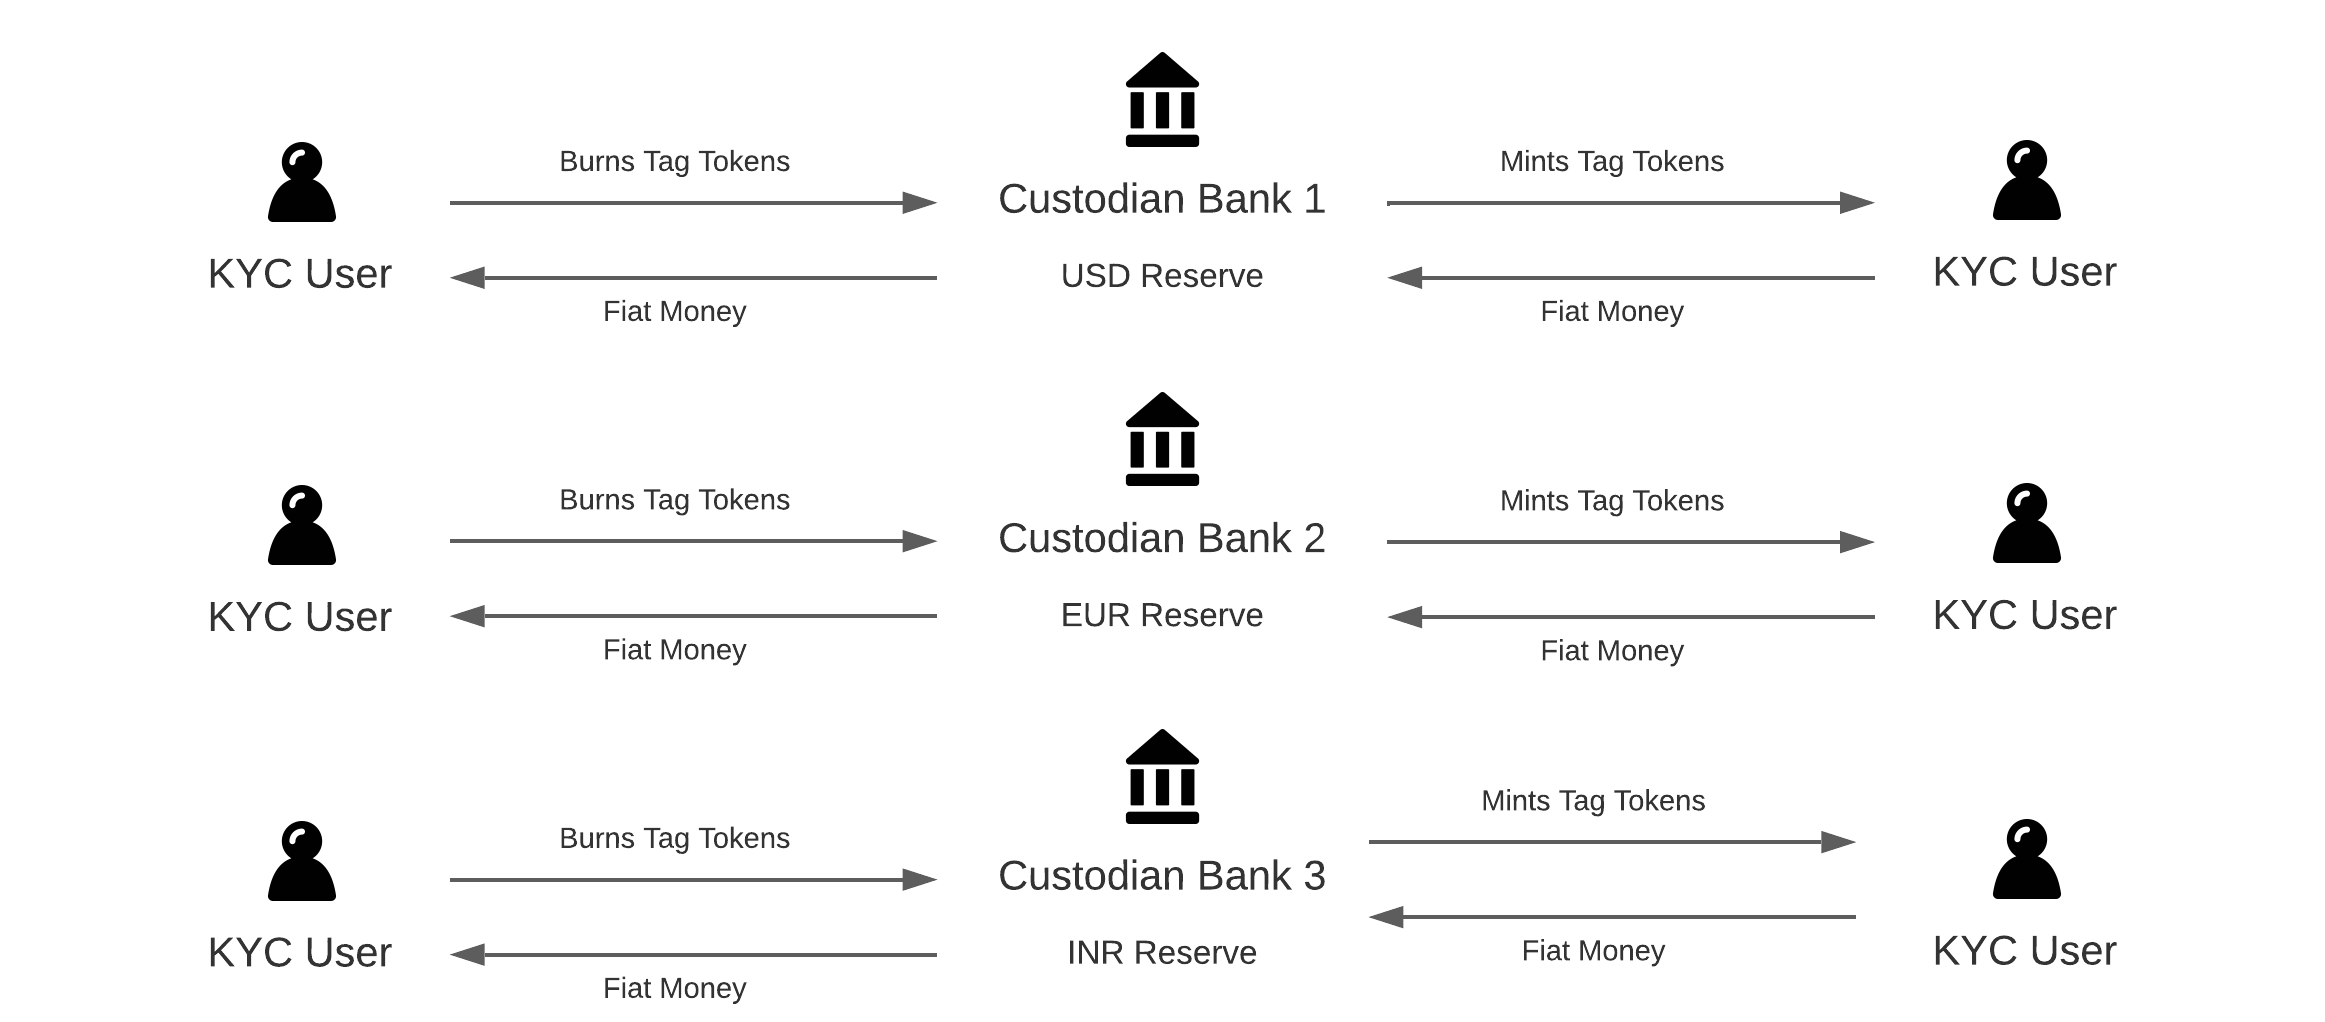
\includegraphics[width=\textwidth]{custodian}
\caption{Fiat Funds Custodian Banks}
\end{center}
\end{figure}

\textit{Example}\\\\
Deposit = \$150 ; Method:Bank Transfer\\
$Total\:Mint=150-0 = 150$\\
Total Mint = 150 USD Tokens\\
$Total\:Token\:Distribution=150-(150 \times 0.1\%)=149.85$\\
Total Distribution = 148.85 USD\\
Total Fee = 0.15 USD ; Custodian Allocation = 0.105 USD\\

\textbf{Exchange}\\

Viral-FEX makes use of ViralDEX Swap Book DEXs for exchanging Tag-Tokens to Viral Coin \& Viral Stable Coin. While Centralized order book exchanges holds user's private key, viral-fex supllies tag-tokens that can be exchanged for viral primary coins using a decentralized efficient White-listed liquidity pool specifically for KYC Users.\\




\textbf{Burning Tag-Tokens / Fiat Withdrawal}\\

Fiat-Tag Tokens are burned upon Cash Out request from the KYC User to the corresponding custodian. The Custodian shall burn the tokens excluding the withdrawal fee and maintain the equilibrium of assets on both bank reserve and token circulating supply. The KYC User is required to add bank accounts or payment ids for the stipulated fiat-money i.e., Burning USD requires USD Bank account integration. 


\subsection{Custodian Services}

\subsection{Business-Wallet API and SDK}

\subsection{Other Wallet Features}

\textbf{QR Pay}\\

The need for faster transactions is rising higher every year and new technologies have been introduced such as NFC, Scan Code, etc. Since Viral Wallet is a crypto wallet, it will be hard for people to use a public address to send and request Viral Coins or other cryptocurrencies to Merchants using the Smart Wallet . QR Pay is a feature to be added on the Smart Wallet to facilitate faster recognition of seller’s wallet address and the amount to be transferred by scanning a simple generated QR Code through Viral Application. This QR Pay will come when the user doesn’t know their username and want to request money from a nearby person. This will be helpful for businesses to collect payment from users swiftly by entering the amount needed to be paid.\\

\section{Child Platforms}


\subsection{Content Moderation Platform}



Centralized social media holds the administrator rights of users’ data which circulates in their platform and also misuses their authority by deleting or expelling a certain user from posting content. This effectively increases the chance of eliminating individual rights, dealing with governments, and most importantly losing the trust of the people. Usually, content moderators on existing social platforms will be held responsible for removing illicit content whereas sometimes due to a centralized approach these moderators are told to filter independent content posted by creators on certain topics where the companies works with the governments sideways. This is why a decentralized community such as ROV is needed for the Viral Network to automate the process by giving administrative rights of the source-uri of contents inside the Viral-Alpha Application to a swarm of moderators which is going to be the key for independent content and removal of explicit contents in a faster and democratic way possible.\\

ROV is an abbreviation for Republic of Viral, a decentralized community-based organization inside Viral Network to govern, filter out reported contents, give support to users, verify VIPs, vote on involvements of community members, etc. The Community is solely developed to bring a decentralized way of allowing a network of administrators under a voting mechanism to remove NSFW, spam content in the Viral Network, and aims to create a cleaner social media while restraining the power of censorship resistance. \\

ROV is designed for curators to work as employees of an organization with a common goal with maximum trust and anonymity. This decentralized way effectively reduces the opinion of a single person, an entity’s founder, and any external influence where the community only decides which is better for the platform. ROV eliminates the need for a centralized entity to run a social platform that holds the power of democracy while ignoring censorship resistance. \\

\textbf{Moderation and Manual Removals}\\

To remove a post in centralized social media, the entity governing the application shall remove the user's database tables that contains the post-meta data. Post Metadata is defined as the data providing information about one or more information about a post i.e., image url, description, etc. Unlike centralized social media, Viral is a decentralized social media that doesn't owns user's data, hence Viral and it's developers doesn't have governance over users meta-data. For a clean, appropriate content platform moderation is a key for it's growth. Viral proposes to solve moderation issues by removing the media's source from it's following storage nodes i.e., Private IPFS Cluster.\\

\begin{figure}[H]
\begin{center}

\begin{forest}
  forked edges,
  for tree={edge+={-Latex}},
  [Viral
    [Alpha-Release
        [Private IPFS Clusters]
    ]
   [Beta-Developers
        [IPFS Public Nodes]
    ]
  ]
\end{forest}
\caption{Available Viral Application Releases}
\end{center}
\end{figure}

Viral Release Applications are separated into two divisions that will have two methods of storing media in the decentralized way possible. Viral Beta-Developer Application resides Open-source as a repository for developers where it will be publicly accessible—anyone can see, modify, and distribute the code as they see fit. The Beta-Application won't be available in mobile application stores and will use IPFS public nodes to store the media. IPFS — a peer-to-peer distributed file system where all files in the public IPFS network are accessible to everyone which cannot be tampered, removed or moderated at any cost. \\

Viral Alpha-Release is the furninshed battle-tested application that will be available in all stores for users. The alpha-release will be using IPFS private cluster, to pin files from public nodes and store public data privately for moderation purposes. The private network cluster allows IPFs nodes to only connect to other peer nodes with shared key, and the nodes in the network do not respond to the communication from nodes outside the network. Cluster replicates and tracks pins across a cluster of private IPFS daemons. In short, The Beta app uses public nodes replicates, store data publicly where it cannot be removed, the alpha app uses private cluster that replicates data from public nodes to a swarm of private nodes that is kept within the ViralDAO where the private nodes are notified by ROV to remove pins(media) from the private nodes. Combination of a fully decentralized storage and a semi-centralized storage to combat illicit content\\


\textbf{Removal Poll Timer}\\

To ensure faster removals and counter the delay of manual approach of votes calculation, after content is reported it will be directly posted on ROV’s Application where the voting poll for the specific post timer will run according to the category’s emergency for removal. This ensures faster content removals in no time, where it takes 24 – 48 hours for a centralized social media entity. We have listed out the major categories and timings for reporting illicit content in Viral.

\begin{itemize}[leftmargin=+0.2in]
\item Spam or Fraud – 2 hours
\item Bullying or Hate Speech – 45 mins
\item False Information – 1 hour
\item Sexual Harassment - 30 mins
\item Nudity – 30 mins
\item Violent or Disturbing – 30 mins
\item Something Else – 2 hours
\end{itemize}

\textbf{Algorithmic Automated Removal Methods}\\

Additionally, to improve faster removals we will be rolling out another AI feature that finishes the poll timer if the votes are more than 10 (Eq 19) and 95\% have voted to remove content or keep content (Eq 20,21). This effectively eliminates the possibility of waiting to remove the content till the timer ends, if the post is in a high state of emergency to remove. There will be an AI feature also to filter out nudity content on the platform automatically without any votes.\\

\begin{equation}
Total\:Votes\:(x) \geq10
\end{equation}
\begin{equation}
(\frac{Total\:Remove\:Votes\:(r)}{x}) \times  100 = r_p \geq 95
\end{equation}
\begin{equation}
(\frac{Total\:Keep\:Votes\:(k)}{x}) \times  100 = k_p \geq 95
\end{equation}

$r_p$=Remove Votes Percentage, $k_p$ = Keep Votes Percentage\\

\textbf{Separate Application}\\

ROV will be having a separate Mobile Application for curators and moderators to easily vote for reported contents using swipe methods similar to dating apps. Since ROV is a restricted content application it will not be available on the mobile applications stores. The Application will be only available on Android as a 3rd Party App and won’t be available for iOS devices due to their security policies. This application will be providing productive features for curators to vote on moderating reported content. \\

\textbf{Process of Polls}\\



\begin{figure}[H]
\begin{center}
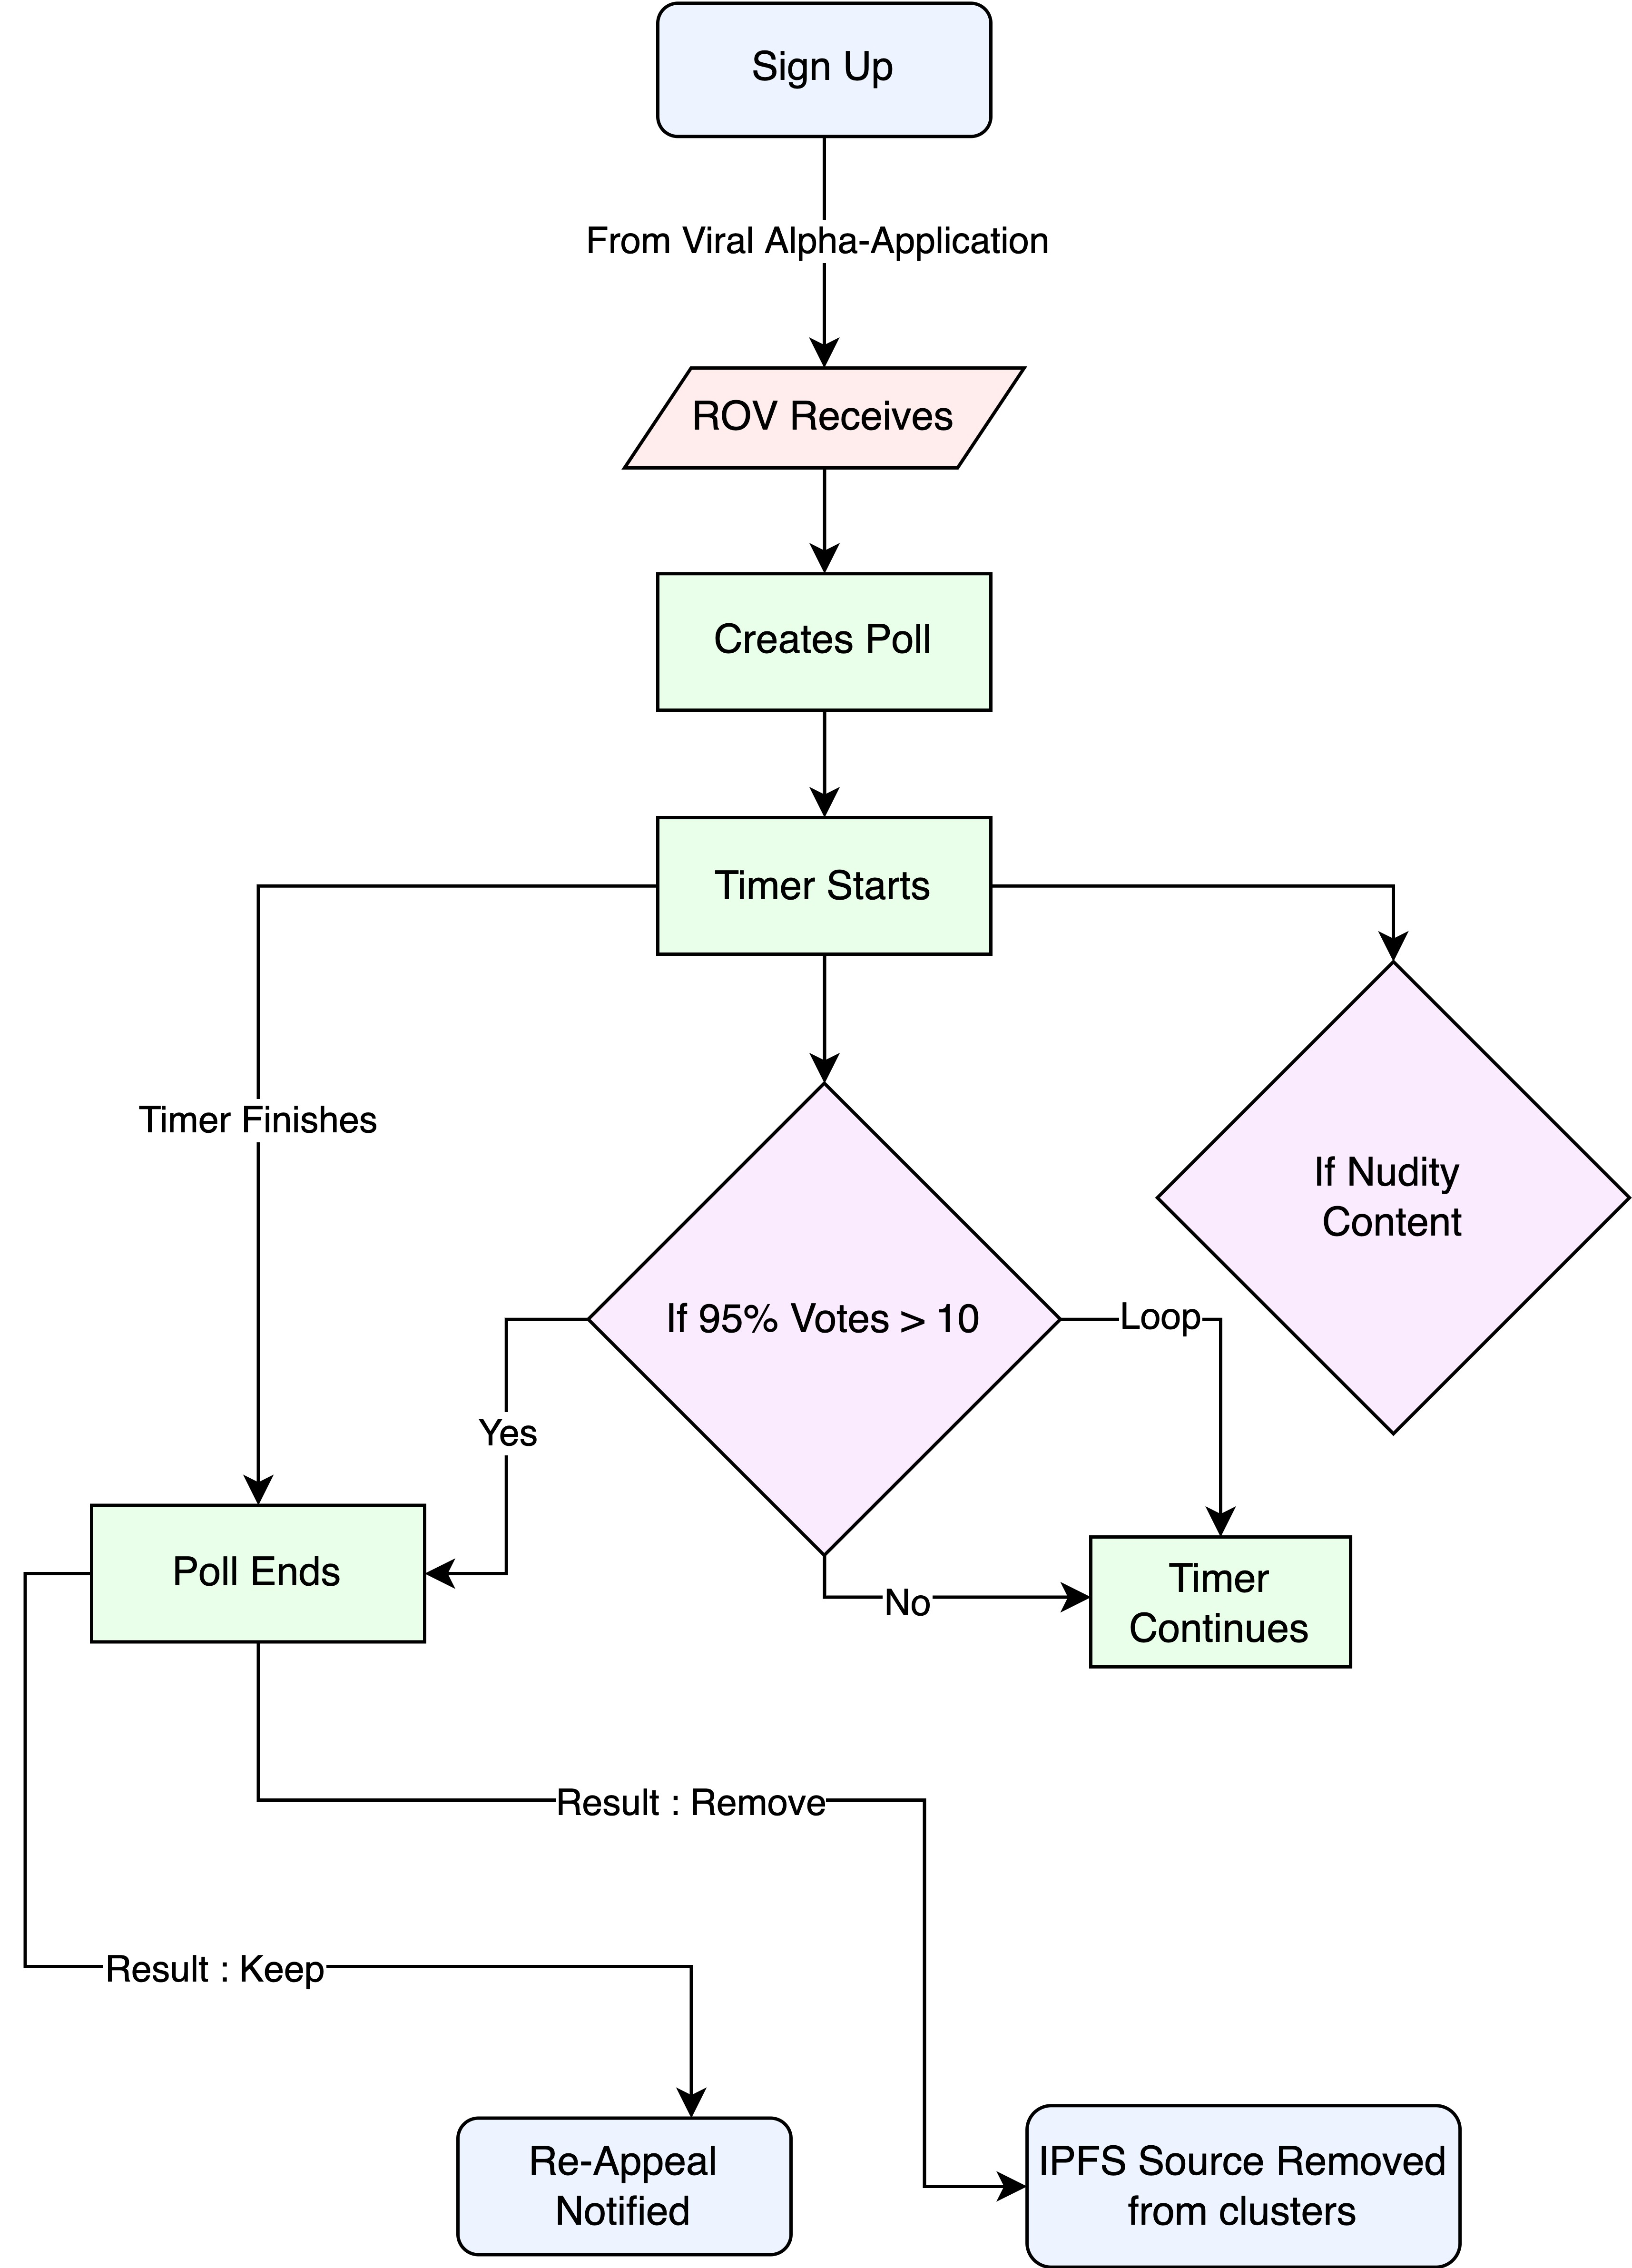
\includegraphics[width=8cm]{rov-poll}
\caption{Glimpse of ROV Process}
\end{center}
\end{figure}


\begin{comment}%rovgrpah

%mermaid graph https://mermaid-js.github.io/

flowchart TB

A([User Reports])--From Viral App-->B[/ROV Receives/]
B-->C
C[Creates Poll]-->D[Timer Starts]
D-->E{If 95% Votes >10}
D-->|Timer Finishes|H
E--no-->G[Timer Continues]
E--yes-->H[Poll Ends]
G--loop-->E
H-->|Result: Keep|I([Re-Appeal Notified])
H-->|Result: Remove|J([IPFS source removed])

\end{comment}

\textbf{Re-Appeals}\\

A unique feature of ROV given to the users of Viral to re-appeal or re-report against the decision of voters while giving an explanation where the ROV curators can again vote to keep the content again or remove based on the explanation given by the user who re-reported. The timer for re-appeal is 5 hours per post where if votes are more than 25 (Eq 22) and 90\% opt again to keep or remove the content (Eq 23,24) the timer will end prematurely.\\

\begin{equation}
Total\:Votes\:(x) \geq25
\end{equation}
\begin{equation}
(\frac{Total\:Remove\:Votes\:(r)}{x}) \times  100 = r_p \geq 90
\end{equation}
\begin{equation}
(\frac{Total\:Keep\:Votes\:(k)}{x}) \times  100 = k_p \geq 90
\end{equation}


$r_p$=Remove Votes Percentage, $k_p$ = Keep Votes Percentage\\

\textbf{Private Accounts}\\

Viral’s content reports are only applicable to public accounts. Viral’s vision to bring complete privacy and security to private accounts which are exempted from being reported. ROV curators will not moderate, nor involve to view the contents of secured private accounts. Thus, it leaves decisions in the hands of followers whether to view their content or not. \\

\textbf{Eliminating Bad Curators}\\

To eliminate biased curators we will be bringing a safe mechanism to filter out bad curators in the community using a feature called positive/negative points. Every single poll will contain two options for the curators to select, “Remove” or “Keep”, the poll results are based on the majority’s decision. When a vote for a poll and falls under the majority’s vote the curator will receive a Positive point, if the curator is on the minority side, which is the losing side he/she be getting a Negative point. Each of the positive and negative points will be added to his profile. An algorithm will run to take the percentage of both points, where if the negative point falls above 30\% to the positive point, his ROV account will be suspended for a couple of days. We have deciphered the factors where there could be no bad actors in the community. There will be records to everyday's positive and negative points. \\

This Positive/Negative points suspension factor will be running after every single vote after the poll finishes. Some factors determining the suspension are\\

\begin{itemize}[leftmargin=+0.2in]
\item If Negative Point is 30\%- 40\% to the Positive Point – Account suspension for 3 days
\item If Negative Point is 40\%- 50\% - Account suspension for 6 days
\item If Negative Point is more than 50\% - Account suspension for 12 days
\end{itemize} 

\begin{equation}
Positive\:Point(p) \times  30\% \leq Negative\:Point(n) \leq Positive\:Point(p) \times  40\%
\end{equation}
\begin{equation}
Positive\:Point(p) \times  40\% \leq Negative\:Point(n) \leq Positive\:Point(p) \times  50\%
\end{equation}
\begin{equation}
Positive\:Point(p) \times 50\% \leq Negative\:Point(n)
\end{equation}\\

We have also made factors to suspend an ROV account forever based on the number of suspensions they get on their account. The factors are
\begin{enumerate}[leftmargin=+0.2in]
\item 20 times 3 day suspension 
\item 10 times 6 day suspension
\item 3 times 12 day suspension
\end{enumerate}

There will be a test-net and live-net to practice voting at its best\\

Example : \\

User A: Day 26; Positive – 234; Negative – 55; Result: More than 20\%: Suspension for 3 days\\
User B – Day 30; Positive – 523; Negative – 343; Result : More than 50\% : Suspension for 12 days\\


\textbf{Community Help \& Support}\\

ROV will be having a separate section for community help \& support, where ROV curators can easily offer their support to Viral users by providing them answers for their queries through the application. The Curators will act as support persons for their issues and thereby providing answers for their problems. It will be a decentralized substitute for centralized customer support. Since the curators cannot offer custom support by an admin staff in a centralized company rather, they can offer support for their questions regarding the usage of the application. For every contribution by the curators, they’ll receive their fair share of rewards.\\

\textbf{Verification of Accounts of Celebrities}\\

ROV curators also will be responsible for several actions on the decentralized platform, one of it's the "Verification of Accounts". Since Viral doesn’t take a single byte of data, we won’t be requesting any country’s identification information like other centralized social medias, it is up to the curators to opt for giving a verified tick for the VIPs on the viral platform. Curators vote on Providing Verification where the majority votes decide the verification of a specific individual or organization. Users applying for verification can provide additional data such as popular media websites blogs about them, provide a verification video and also tip the rov community on whole to provide verified tick.Verified Tick is represented by a unique NFT minted by ROV using it's pool's reserve and send the nft to the user applied for it.\\

\textbf{Requesting ROV}\\

Since ROV is regarded as a DAO (Decentralized Autonomous Organization) we make sure others request ROV for a specific task, poll, support, etc. This feature will be given only to verified profiles where they can write to ROV in any matter where the curators can come collectively to help regarding the issue. This will help VIPs, Governments to write to ROV curators which will be displayed on their feed where they can take necessary actions for it. \\

\textbf{Rewards for Contribution}\\

Every day according to every individual curators contribution rewards will be allocated to their wallets where they can collect it manually after 2AM UTC. 


\subsection{Developer Platform}

Viral Dev-Space is a platform for developers to develop, communicate together with other experts, and receive rewards for their contribution to the Viral Open-Source applications and future development plans of the public and the Viral DAO. The Space for developers is created to decentralize and automize the Software Research \& Development sector of Viral Applications in an efficient way by providing rewards in Viral Coins through unbiased voting based on the intensity of their contribution and popularity in the development community.\\

Viral will be providing an opportunity for all developers regardless of their educational background, region, and language to work on improving the viral decentralized applications on fields such as security, interoperability with other social giants and also to make the application bug-free while providing new updates to the beta software which will be available as an Open-source repository. Giving new opportunities to develop for an upcoming massive social network will pave a way for fastening the development process by using the potential of mass development techniques.\\


\textbf{Short Benefits}:
\begin{itemize}[leftmargin=+0.2in]
\item Full Automation on Research \& Development
\item Potential of a bigger development community
\item New, Exciting Unknown Developments for the application
\item Shorter Time for fixing bugs and issues
\item The cost of Development is considerably low
\item Decentralized HR \& Rewards according to the contribution
\item Expedite the Development of Viral Future Plans
\item And many more advantages to receive a contribution for the application’s source code in trade for daily rewards
\end{itemize}

\textbf{Allocation of Rewards}\\

The rewards are based on democratic voting where every developer will have their own project feed to appreciate the work of other developers. There will be an engagement feature to “Like” the contribution they’ve pushed to the code repository. After a developer makes a commitment to the repository by pushing his/her code and after the merge, their work will be posted on the project’s main feed. At the end of the day every 24 hours, the amount of likes every post received by the user profiles on all the projects will be taken to segregate the amount of rewards per developer. Refer Rewards section for detailed information on the segregation of total revenue separated for developers.\\

\textbf{Application}\\

Viral will provide a web application where developers can join, interact in development groups and receive rewards daily every 24 hours according to their contribution. This application will be maintained by Viral DAO. The App will serve as a community platform where any developer can choose their favorite preferences, communities, and development projects. Developers can choose the project of their preference by searching and also by opting for an interactive questionnaire to find out which project is suitable for them. After giving their preference they can choose the project they want to work in. The developer will have a limit of working on two projects at a time, where they can remove themselves from the project team and opt for other projects as well. This will ensure that developers will have an increased productivity and a higher success rate in specific projects.\\

\textbf{App Features}\\

\begin{itemize}[leftmargin=+0.2in]
\item Choosing preferred project
\item Collaborative Workspace for Developer Teams
\item Easy Work-Management
\item GitHub Account Integration
\item Private and Project Group Chats
\item Add New Projects to Dev-Space by providing a whitepaper
\end{itemize}

\subsection{Viral Decentralized Ads}

\subsection{Influencer-Ad Platform}

Mainstream modern-advertisement focusses on targeting social media users by running campaigns collaborating between brand and influencers. It takes the idea of celebrity endorsement and places it into a modern-day content-driven marketing campaign. This type of marketing doesn't only involves celebrities but popular content creators who have an enthusiastic audience. Influencers can be anyone anywhere but what separates them from a amateur creators is their large following. Some will have hundreds of thousands, some even millions, brands do care their reputation build around the specific industry that they are looking for i.e, Fashion, Comedy, Sports. They are the people who make engaging contents, share the best pictures, entertain their viewers, run exciting discussions across social platforms on their own specialized topics. From a smaller market size of \$1.6 billion in 2016 it rose to a figure of \$13.8 billion industry in which for every \$1 spent businesses receive purchases worth \$5.78 from all over the world giving an ROI (Return of Investment) of 500\%. About 1360+ Influencer marketing focused platforms and agencies entered the market in the last 5 years alone.\\

Viral Influencer Ad-Platform is a place where influencers get connected with brands and businesses under specific requirements to place paid-ads by determining per-impression rates where Content creators can post brand ads under specific categories such as impressions, engagement, link clicks, etc so brands can purchase with the trust of the blockchain. After the promises of the gig are achieved the payment will be released to the influencers. This effectively reduces the unwanted issues regarding promised results. Viral will be tapping the potential of influencer marketing by running ads through popular content creators. We want to effectively eliminate the excess process of a business to find influencers, contact, fix, transfer amount, etc into a simple user-friendly platform where it can
\begin{itemize}[leftmargin=+0.2in]
\item Find tailored Influencers with advanced search algorithm
\item Payment using Viral Pay and multiple available tokens
\item Check Realtime-statistics of the ad
\end{itemize}

\textbf{Influencers}\\

Businesses looking for influencers for their next ad-campaign shall look in terms of followers count on a specific profile where larger brands involve bigger influencers ($\geq$ million followers) and medium enterprises involve smaller influencers ($\leq$ million followers). For seamless results in the Viral Influencer Platform the creators are categorized into several categories according to their followers count
\begin{enumerate}[leftmargin=+0.2in]
\item \textbf{Class X} : $\geq$ 10M Followers
\item \textbf{Class A} : $\leq$ 10M Followers
\item \textbf{Class B} : $\leq$ 1M Followers
\item \textbf{Class C} : $\leq$ 500K Followers
\item \textbf{Class D} : $\leq$ 100K Followers
\item \textbf{Class E} : $\leq$ 50K Followers
\item \textbf{Class F} : $\leq$ 10K Followers
\end{enumerate}

A minimum follower count (1K) and a daily impression count is required for signing up in the Viral Influencer Program. Influencers shall provide their per-impression rates on their profiles. Their daily, hourly impression counts are taken into account to display brands and businesses expected ad-result in a certain time period, etc. Influencers can post their per-impression rate on promising certain ad-result for the ad-buyers in easy simple steps. Elite influencers fall onto the category of Class X will be billing higher rates per-impression where smaller Classes will be billing lower rates per-impression. \\

Each Influencer will be classified into niche category. Hashtags of recent posts are taken into account to decide the percentage of posts that is inclined towards a certain category. Sub-categories are also determined for brands to filter and select the best influencer around their target price and ad-performance. Interests of audiences are not taken into any account as Viral is free of data collection systems where the influencer's categories are determined by hastags of recent posts, similarly the influencer can alter his audience interests manually using his/her dashboard.\\

\textbf{Advertising Cost Models}\\

Advertising using Viral Influencer Platform is economic and a better substitution against targeted-ads by social platforms like Facebook, Instagram, Twitter that relies heavily on tracking user's interest to provide them targeted ads. While Platform ads are done aside, the advent of Influencer ads posses more market and provides better ROI and results for the businesses. Viral Influencer Advertising cost depends on various cost models that can be chosen by influencers which is suitable for advertisements. The Models are
\begin{enumerate}[leftmargin=+0.2in]
\item \textbf{PPV} : Pay Per-Thousand Views
\item \textbf{PPC} : Pay Per-Conversion
\item \textbf{PPD} : Pay Per-Day
\item \textbf{PPP} : Pay Per-Post
\end{enumerate}


\textbf{Pay-Per-Thousand Views}\\

PPV is the default pricing option in the Viral Influencer Platform. It is one of the key-metrics of influencer ads which defines "Total Cost per 1,000 views from an ad post" which is used to understand the pricing, ad's effectiveness and performance. Views means total number of times the post is displayed to the users. Views will contain if a single user watches multiple times the same ad post. Similarly additional metrics are given such as
\begin{itemize}[leftmargin=+0.2in]
\item \textbf{Outreach} : To determine the number of users the ad have reached excluding multiple views of a single user.
\item \textbf{Conversions} : To determine the number of conversions such as link clicks that is provided on the caption, etc. Conversion doesn't includes profile visits of the influencer.
\end{itemize}

The PPV cost of influencers are provided upon registration and will be available for brands and businesses to research for their advertisements. Currently targeted advertisements by various centralized social entities are charging \$7 per thousand impressions, viral influencer platform aims to achieve more affordable standard rates over centralized solutions tailoring for each influencer that suits their reputation in the following industry.\\

\textbf{Pay-Per-Conversion}\\

Conversions are suitably links or tags which gets clicked by the user that may funnel them into further actions. PPC ads are used to drive traffic to websites, brand-pages, etc. The advertiser (influencer) charges a fee every time a link is clicked through the ad-post. Essentially PPC is the way of buying visits to your preferred page/website, rather than attempting to earn those visits organically. Influencers can provide their Pay-Per-Conversion rates to their profile which will attract brands to partner and advertise their content in an efficient manner.\\ 

\textbf{Pay-Per-Day}\\

Influencers usually charge payments for running brand ads according to the amount of days the ad-post will reside on their page. Different influencers such as informative pages, meme pages, niche pages attract businesses to pay them for ad posts that will be ran for a certain amount of days receiving quality amount of impressions and conversions to the brand. Influencers can provide their Pay-Per-Day rates to notify brands the best rates for advertising to their followers and new visitors.\\

\textbf{Pay-Per-Post}\\

Pay-Per Post is a simple, direct advertising by influencers, celebrities and models to publish branded-ads by pricing it per post. Influencers can provide their per-post price to directly display how much the cost would be to deliver branded-ads to quality like-minded followers and fans. This direct advertising is preferred by most bigger brands as it costs higher and the ROI is better in terms of other advertisement models.\\

\textbf{Ad-campaign}\\

\begin{figure}[H]
\begin{center}
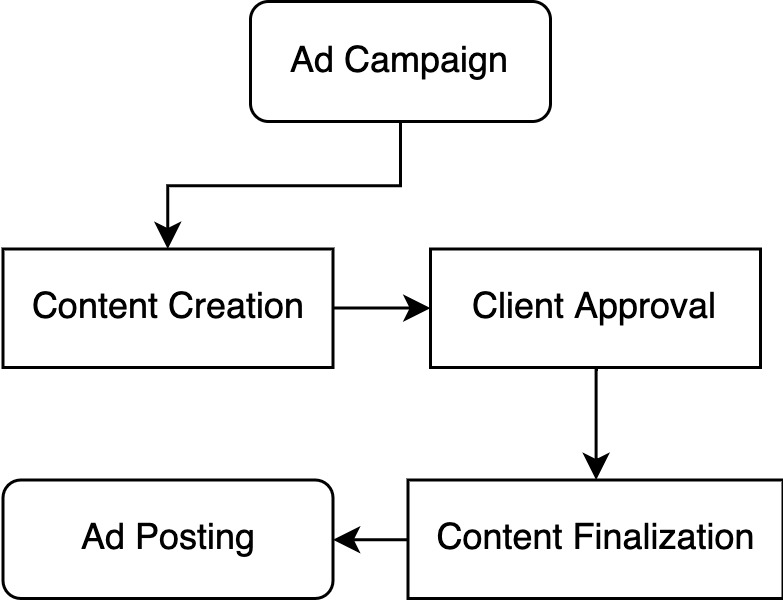
\includegraphics[width=6cm]{ad-flow}
\caption{Ad-Campaign Flow}
\end{center}
\end{figure}

\begin{figure}[H]
\begin{center}
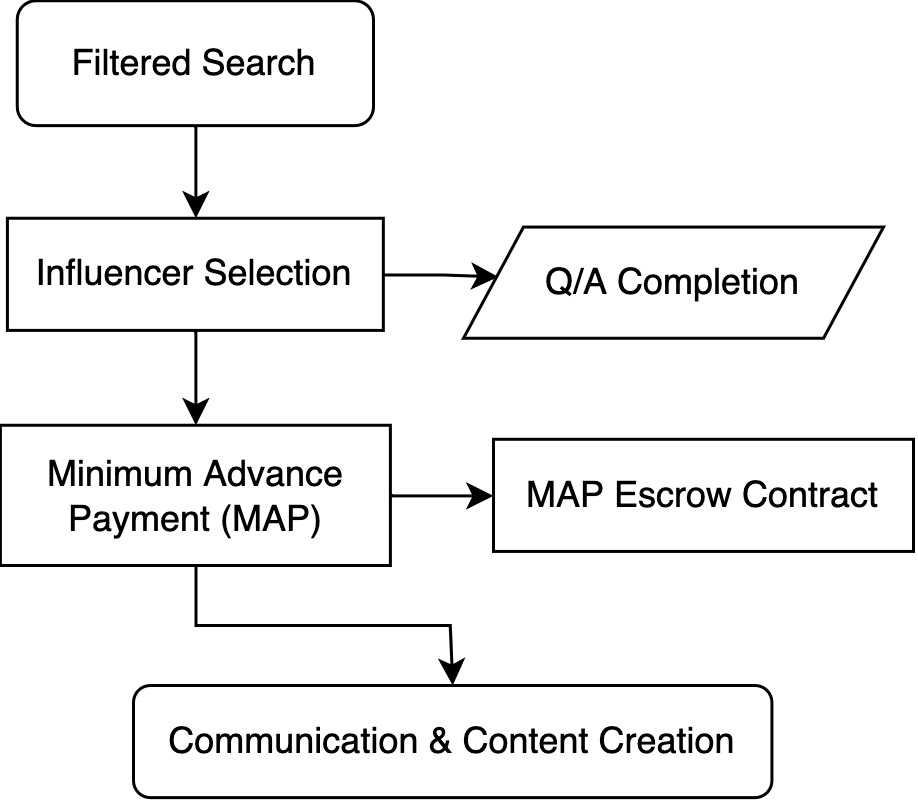
\includegraphics[width=7cm]{ad-selection}
\caption{Influencer Selection \& Initializing Payment}
\end{center}
\end{figure}

\begin{figure}[H]
\begin{center}
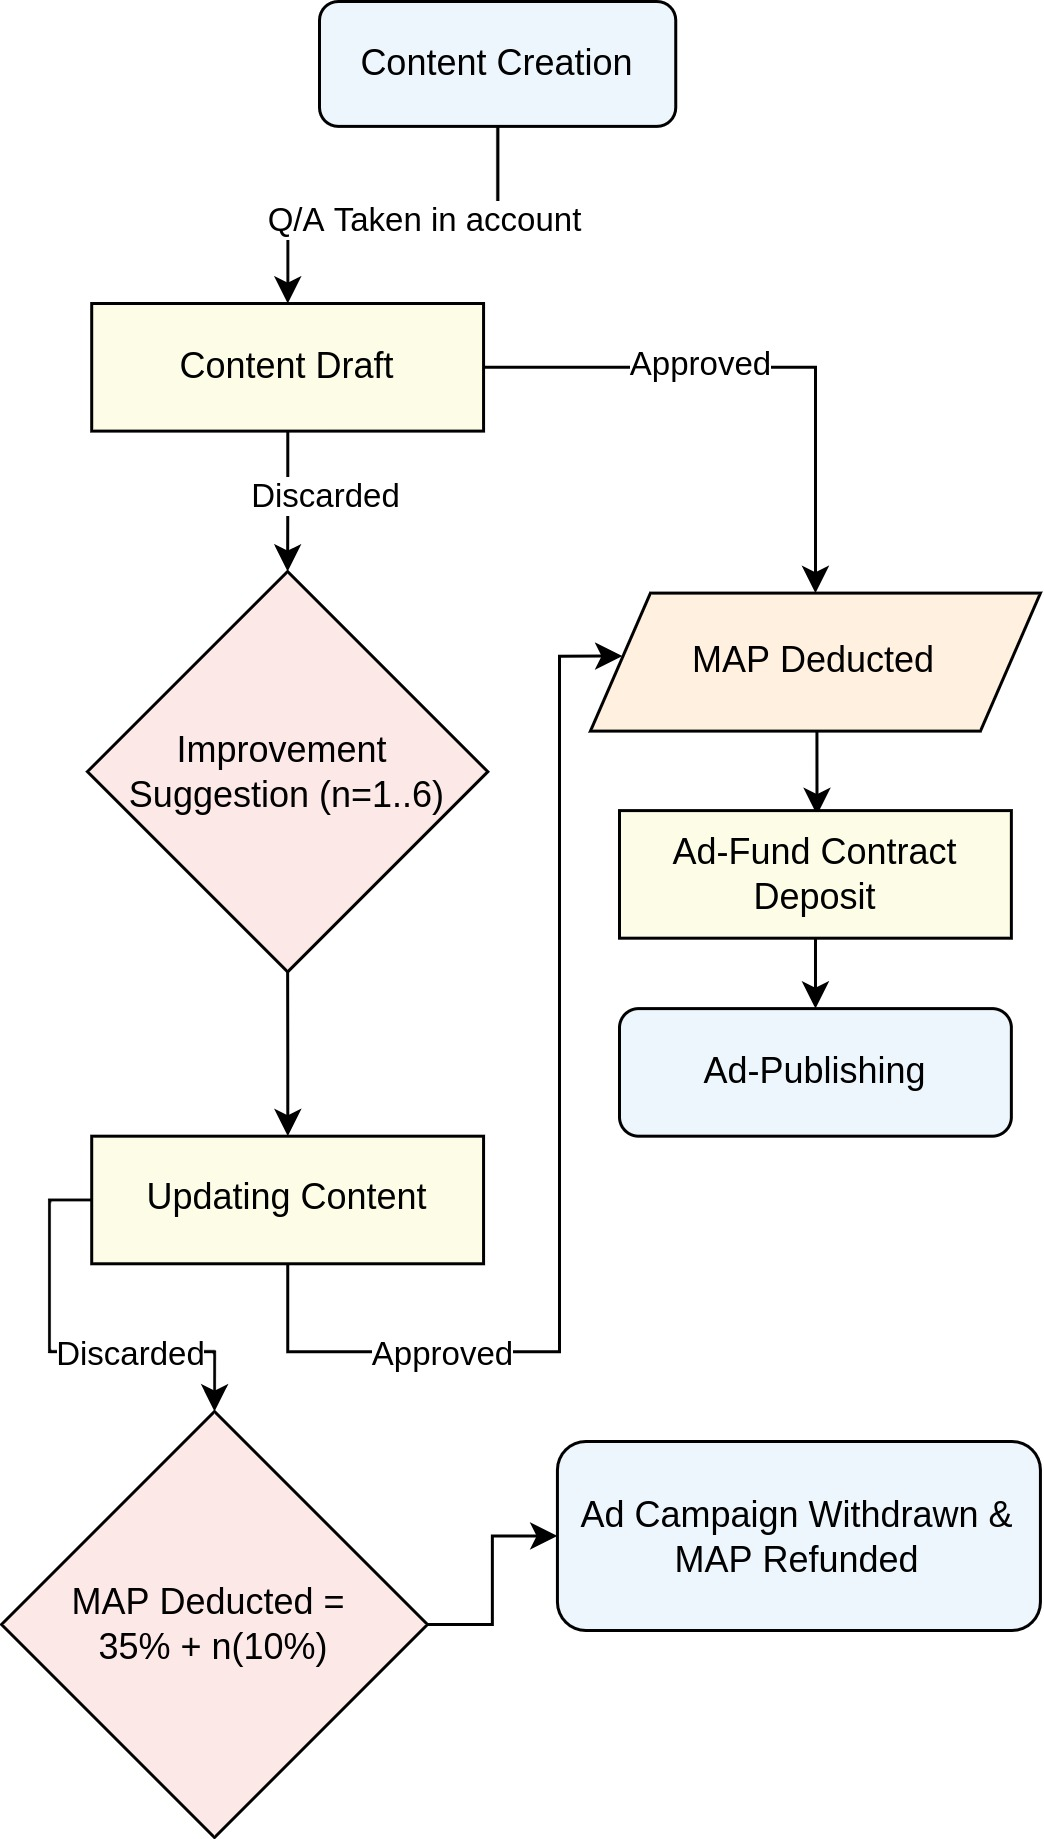
\includegraphics[width=7cm]{ad-content}
\caption{Content Creation \& Cancellation}
\end{center}
\end{figure}

\begin{figure}[H]
\begin{center}
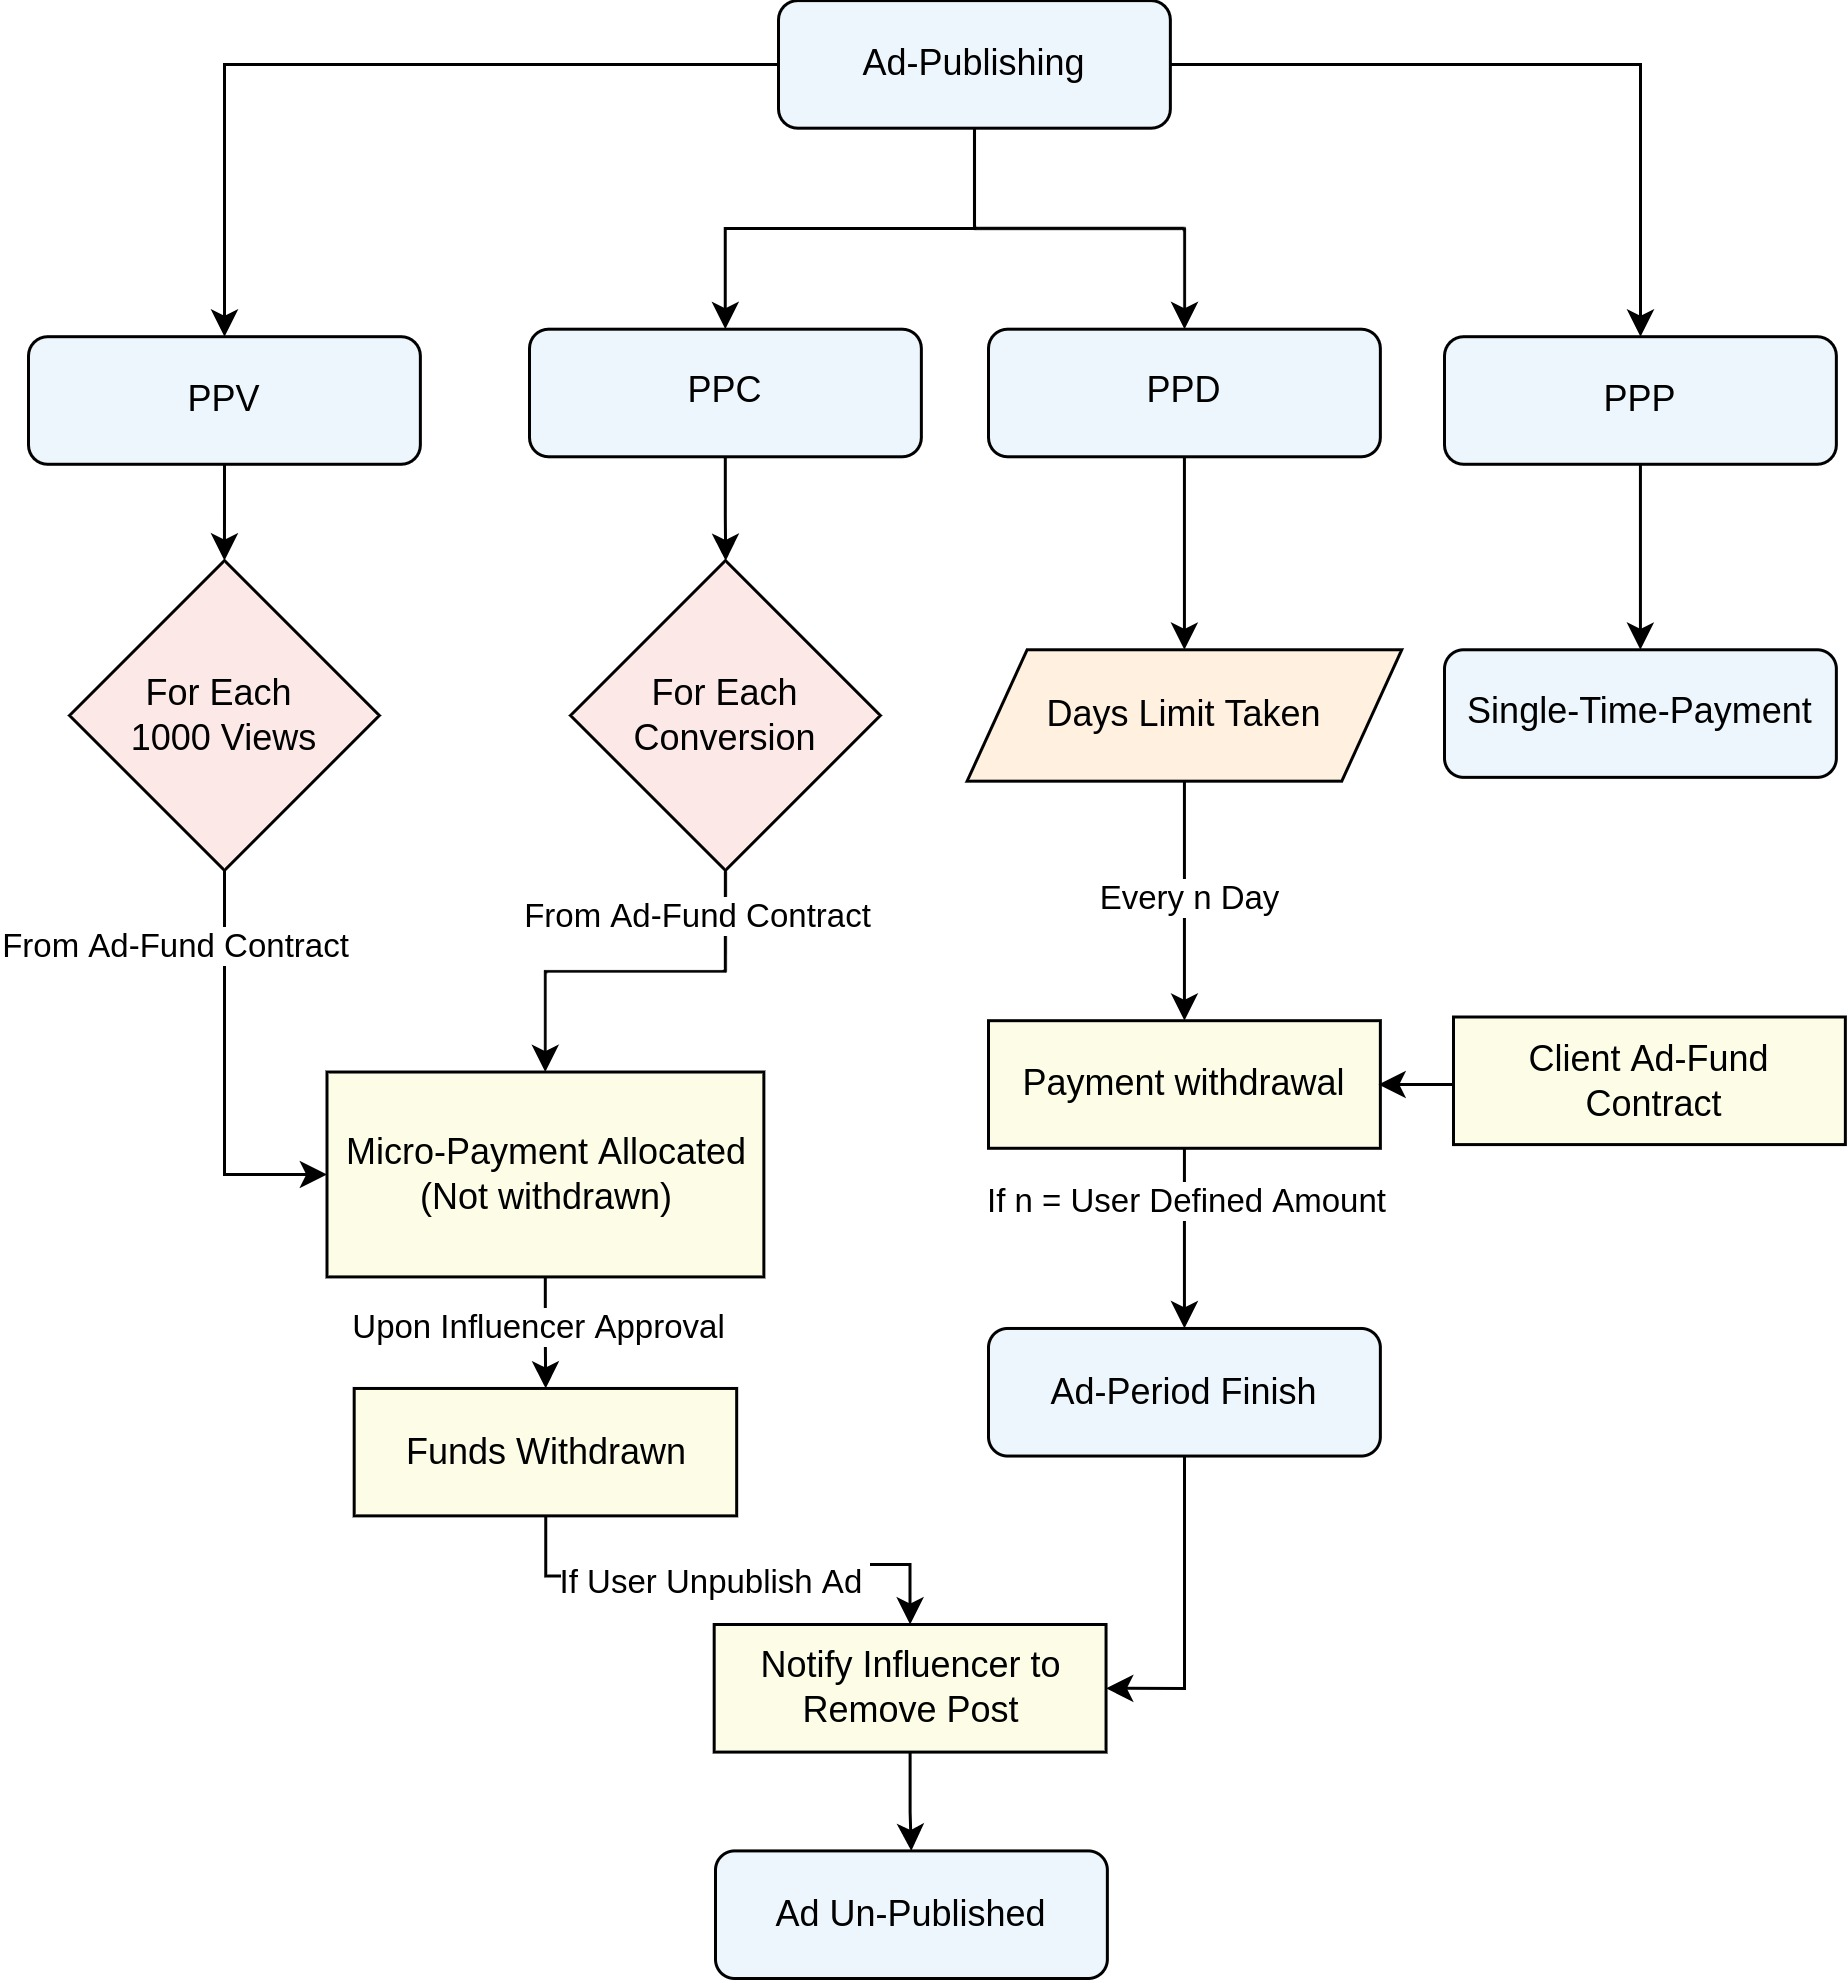
\includegraphics[width=13cm]{ad-publish}
\caption{Ad-Publishing over various payment models}
\end{center}
\end{figure}



\textbf{Fees \& Billing}\\

5\% on inflencer side and 5\% on business side 

\textbf{Benefits of Viral-Influencer Ads}\\




\textbf{How it will work?}
\begin{enumerate}[leftmargin=+0.2in]
\item Business Owners / Individuals / Buyer can search for an influencer account with advanced search filters
\item Finds an Influencer with the list of gigs 
\item Purchases a Gig
\item Amount Paid will be stored in a smart contract (vault/escrow)
\item The influencer gets a notification to create content
\item Buyer reviews the created content and approves
\item Influencer posts the content attributing the buyer
\item The Ad runs successfully and expected engagement by the gig is reached
\item Now the smart contract will release the stored amount to the Influencer’s wallet
\item The buyer gets results, Influencer gets paid
\end{enumerate}


Flowchart\\


Complete Trust\\


If the Gig result is not achieved the payment will not be paid to the influencer. When an individual purchases a gig, he will be paying through Viral Coins where the amount will be securely stored in a vault (smart contract) which is only released to the influencer’s wallet if the gig achieves its result. Here any individual and business owner can be sure that the influencer will need to achieve the result to get paid.\\


Search Filters\\


Influencer Ad-Platform will provide the Business owners and individuals looking for promoting their content on Viral where they can narrow their search to their expected influencers. This makes it easy for individuals and businesses without worrying about the research. We will be providing Filters to narrow down their search as much they can. Some filters are

\begin{itemize}[leftmargin=+0.2in]
\item Account Category (Eg: Food)
\item Fan Base (Eg: more than 1M followers)
\item Account Age (Eg: 6 months)
\item Daily Impression (Eg: 257k views)
\item Country (Eg: Canada)
\item Reviews and Ratings
\item Sort by : Top/Trending/Age/Fans/Impression/Rating 
\end{itemize}


Cancellation and Refund\\


The cancellation and refunds window will be updated by the Influencer on every of their gig where if the Buyer cancels and apply for a refund before the certain hour of posting the picture, the smart contract will refund the exact amount paid to the buyer’s wallet. After the refund window, the smart contract will not refund the buyer. \\


\subsection{P2P Exchange}

Nowadays people want cryptocurrencies without transaction fees, exchange fees, and also without KYC process in an anonymous way. But in order to buy on central exchanges using Fiat-Money, it is not possible without disclosing their personal information and identity cards for Anti-Money-Laundering purposes. Buying cryptocurrencies using fiat money is not possible on Decentralized Exchanges, since it is a platform to swap from one cryptocurrency to another cryptocurrency in a decentralized manner without any centralized order books.\\

This is where P2P exchanges come in. Peer-to-peer refers to the exchange or sharing of information, data, or assets between parties without the involvement of a central authority. These P2P exchanges work on connecting two users nearby around their city, area, who are willing to sell and buy crypto tokens for fiat currencies. Thereby making an agreement of holding the seller's cryptocurrencies in a smart contract to verify sellers and withdraw to buyer until he transfers the fiat-currency funds to the seller and gets confirmed.\\

\textbf{Advantages over Centralized}
\begin{enumerate}[leftmargin=+0.2in]
\item Peer-to-peer transactions generally do not require the involved parties to provide identification,  protecting everyone's right to privacy. 
\item P2P exchanges allow the purchase of cryptocurrencies through the regional medium of exchange that the seller opts for (E.g. PayPal, Square, M-Pesa  etc). Viral offers P2P solutions to all countries' local payment methods for the users without any hassles.
\end{enumerate}

\textbf{P2P for Sellers}\\

Seller listing will be initiated by the token seller. The tokens are allocated on a escrow smart contract that will be holding the funds which can be only withdrawn in the account of closing the listing. Non-sensitive information such as City, State, Country shall be provided upon listing which is preferred by buyers for smooth trade of tokens offline. The Regional Payment Methods are selected and the listing is created. The listing consists of Token name, Tokens amount, Payment methods and City.\\


\begin{figure}[H]
\begin{center}
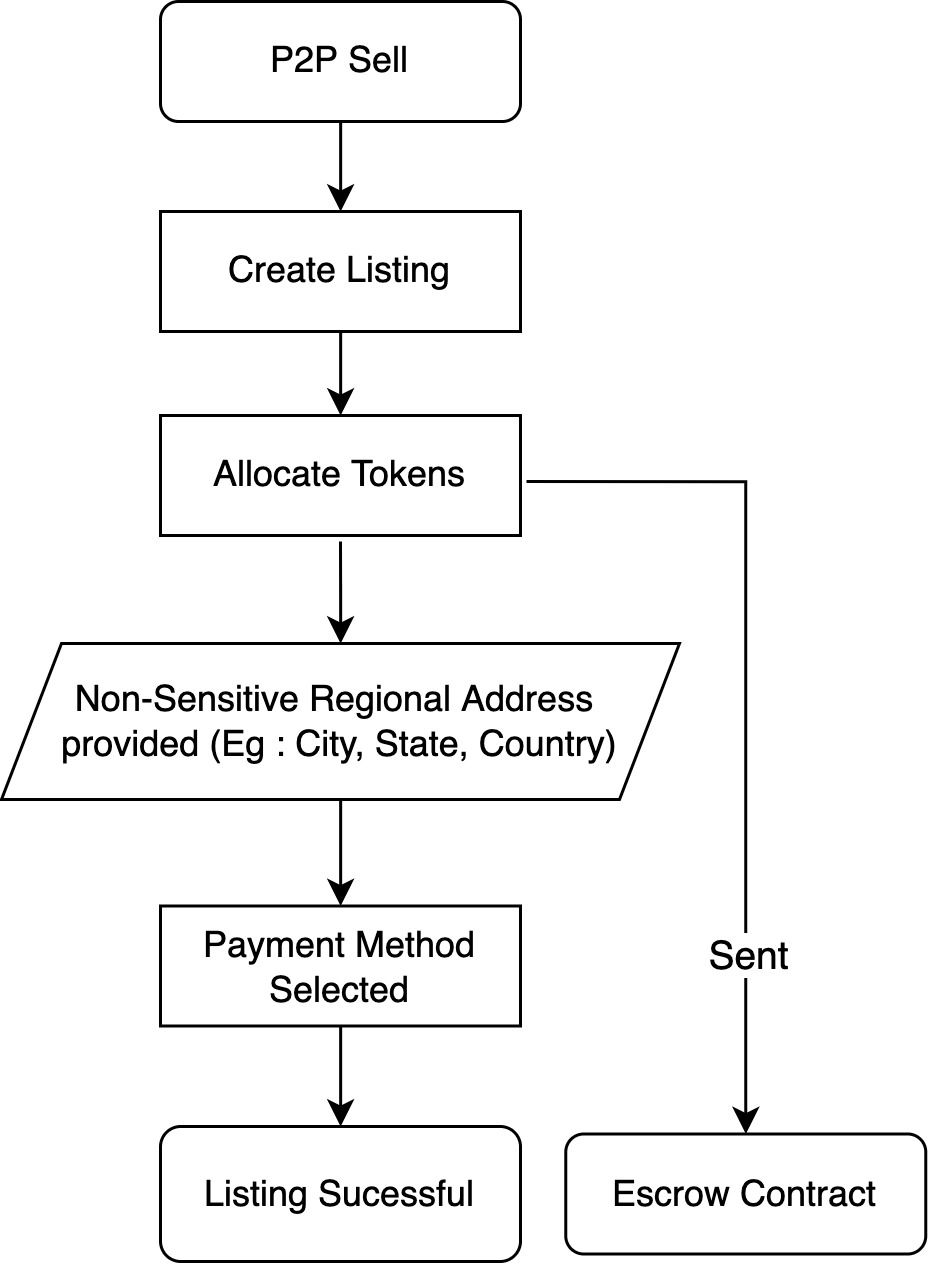
\includegraphics[width=7cm]{p2p-sell}
\caption{Selling Tokens via P2P}
\end{center}
\end{figure}

\begin{lstlisting}[caption={Token Sale Listing}, numbers=none]

	listing id: 02698 {
	
    	"token-id": "vrl",
   		"token-ticker": "VRL",
    	"token-amount": "7289.375",
    	"city" : "Los Angeles"
    	"state" : "California"
    	"escrow-contract-id" : "vy89xfwieug2t8793br9hd2by2dfg"
    	
	}
\end{lstlisting}


\textbf{P2P for Buyers}\\

Users can buy tokens in a secured anonymous manner by connecting with sellers using the P2P Viral Exchange. The Location shall be provided by the buyer to list all the potential seller listing that can be selected upon confirmation by the buyer. The buyer will be immediately connected with the seller by initiating a chat. All the sell listing on the Viral P2P exchange are verified by the escrow smart contract balance which will hold exact value/balance of the listing which offeres a trustless solution for the buyer. After the chat is connected, the seller and buyer shall communicate with each other and provide locations to visit in person or to agree on terms for ssmoother trade without conflicts.\\

The Buyer enters the amount of tokens he would like to buy and the current market price is fetched for the buyer. After the buyers sends the fiat payment, the buyer shall confirm his/her payment. The Seller refers the fiat payment and confirms it. After the confirmation from both parties the contract is revoked and the specified amount of tokens will be sent directly to the buyer's Viral wallet.\\

\begin{figure}[H]
\begin{center}
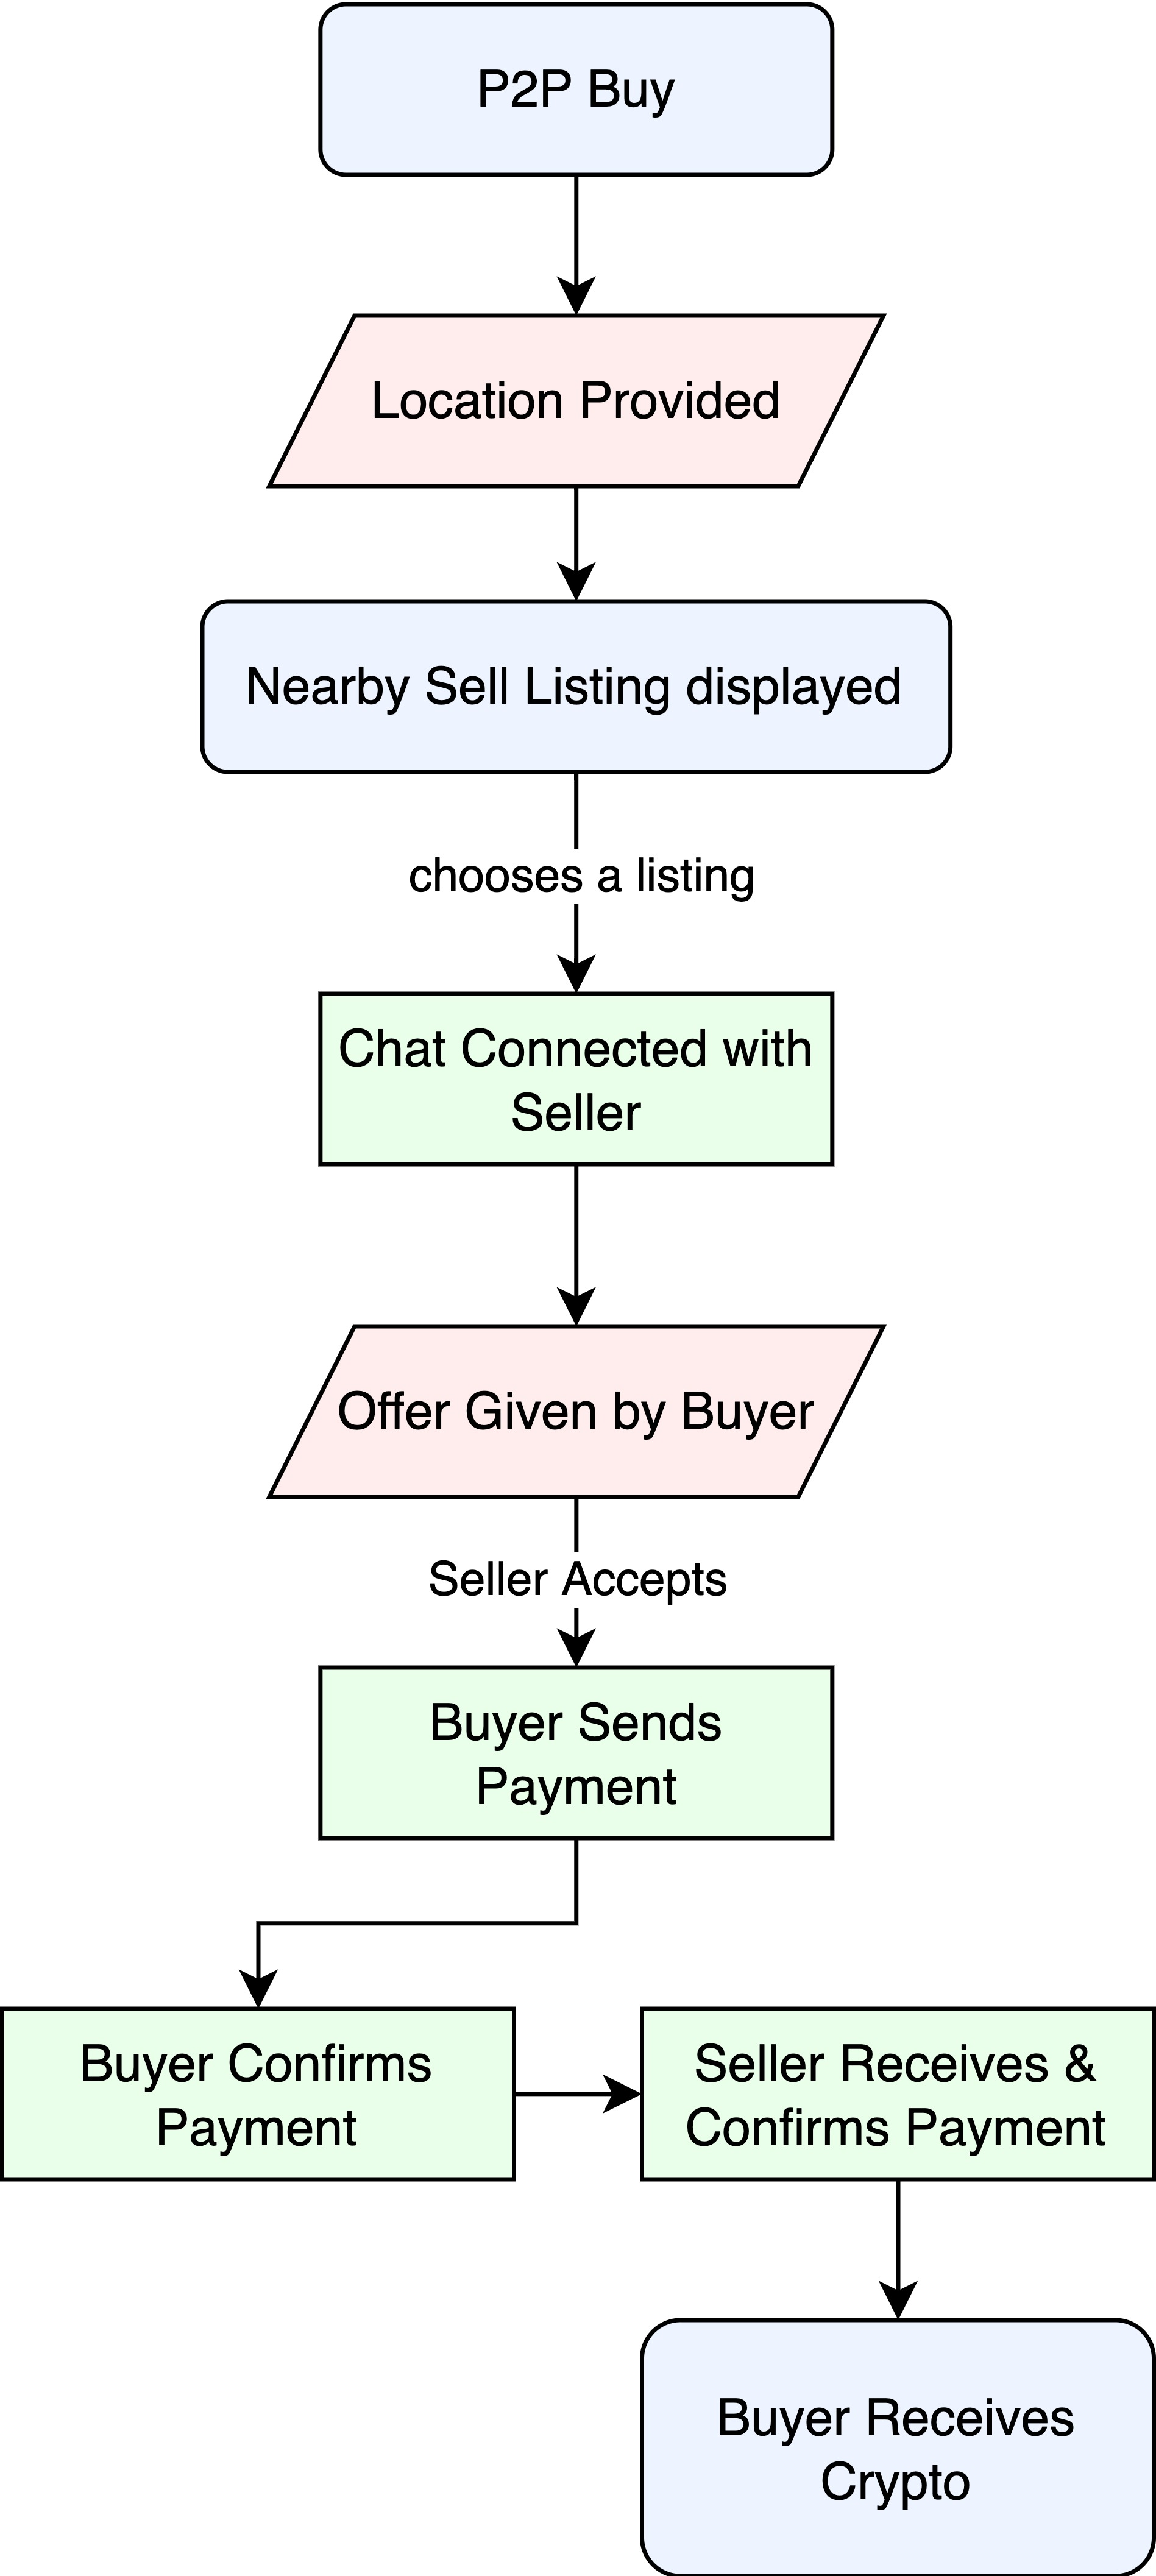
\includegraphics[width=6cm]{p2p-buy}
\caption{Selling Tokens via P2P}
\end{center}
\end{figure}

Our ultimate vision is to develop a decentralized social media without any central authority or a need for a company to run its product, a P2P Exchange will carry out its process of buying and selling Viral Coins for Fiat money. This ensures the trades cannot be banned nor withdrawn no matter what the land rules are.\\



\section{Global Reward Pool}

Viral Rewards are daily rewards allocated to every user on the decentralized platform who contributes towards running the platform. It includes Users, Miners, Volunteers, and DAO Members. Since it is a decentralized platform, it requires no maintenance and authority by a centralized entity. The contribution of every single individual user is needed to run the platform seamlessly. We would be giving out rewards in Viral tokens and Wrapped tokens of popular cryptocurrencies such as Bitcoin, Ethereum, Solana, etc for all the users who contribute towards running the social and multi-chain platform.\\

The Reward allocation for each user happens through automated smart contracts every day at 2 AM UTC. Viral Rewards are designed in such a way that every single contributor inside the network will get paid for their contribution through a either democratic voting system or mathematically predicted points. These points prediction program will be calculated from off-chain real-time data through decentralized tamper-proof oracles in a secure  manner to ensure fair rewards to each user without any influence, third-party recommendation, or external factors. 

The 100\% percent of total daily revenue is distributed as \\
\begin{figure}[H]
\begin{center}
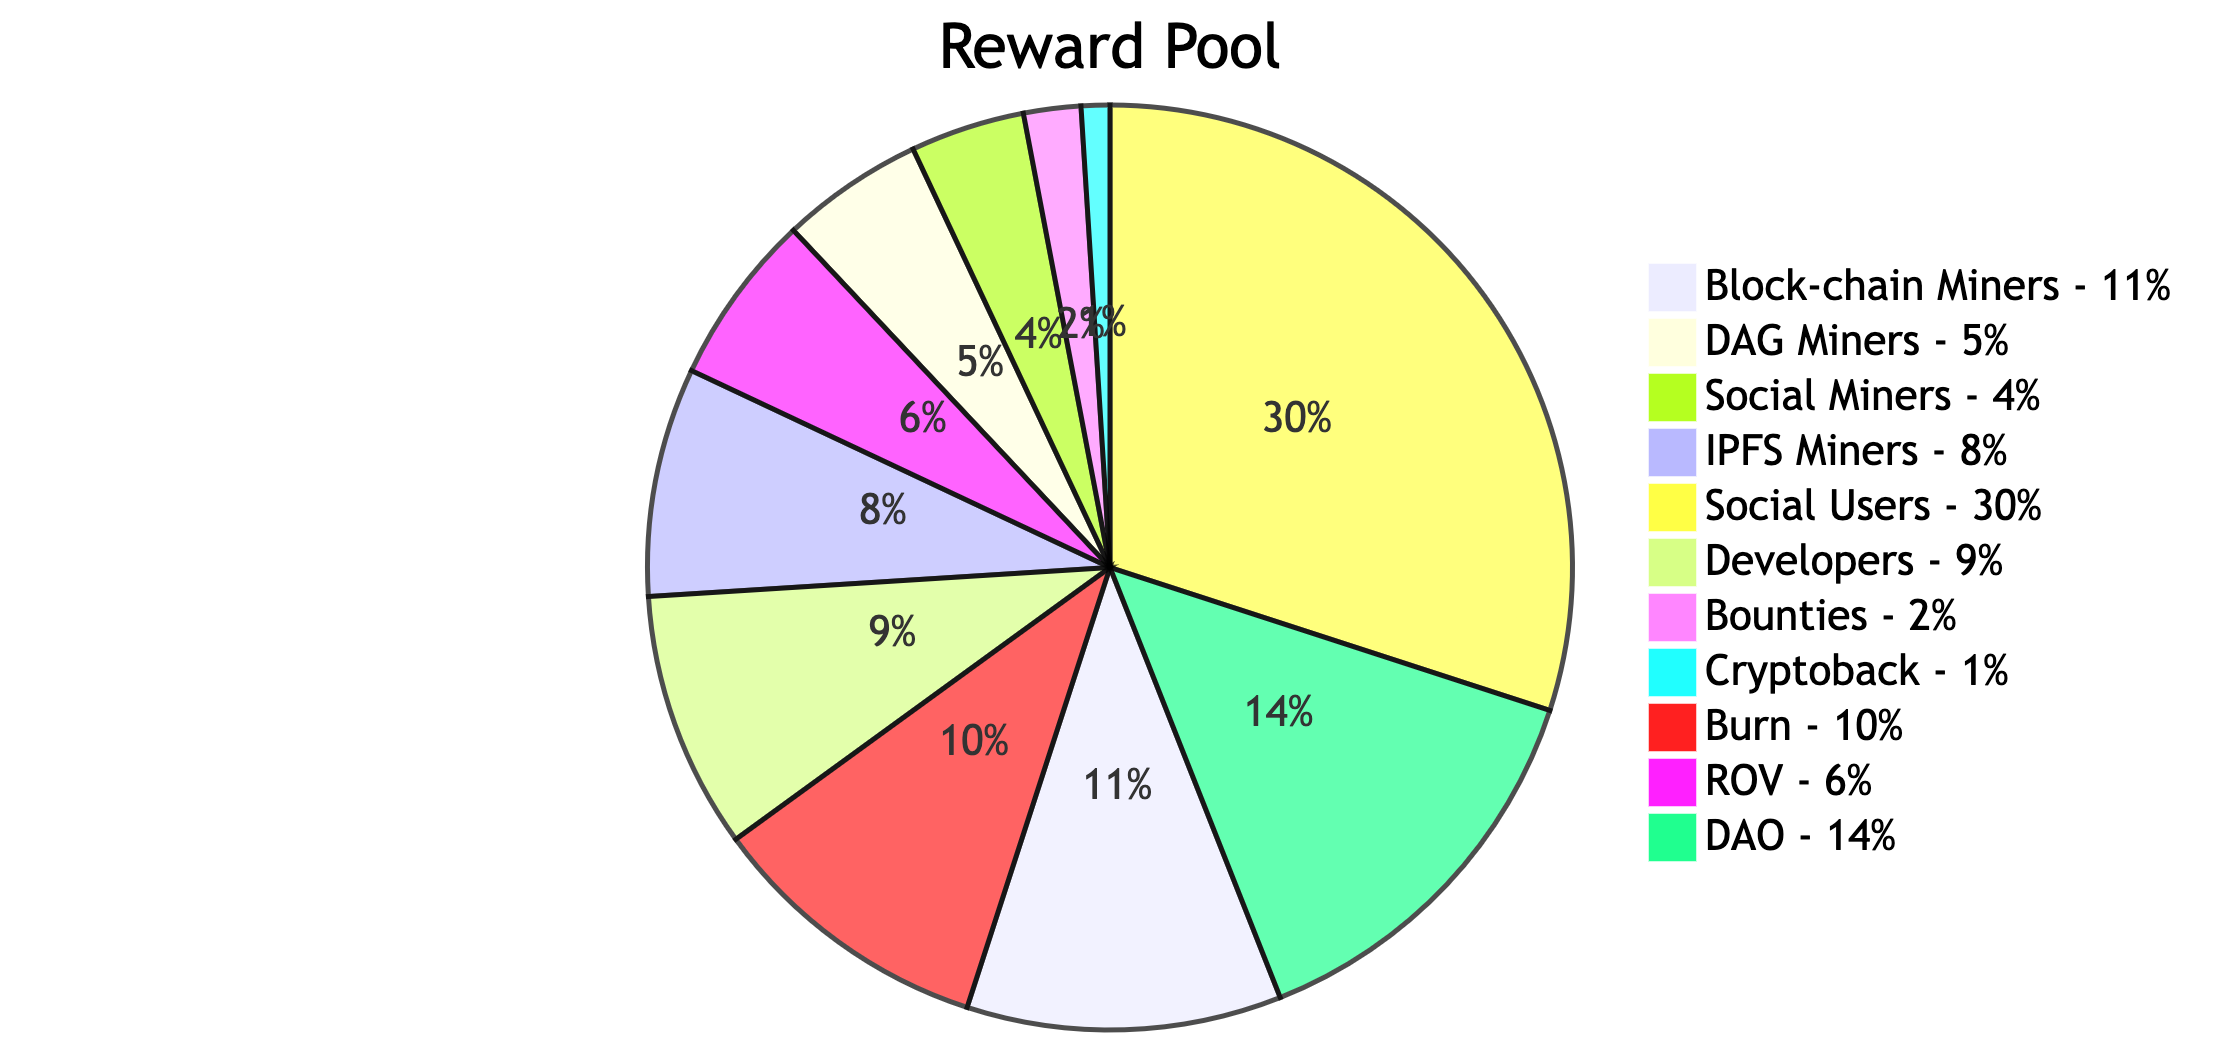
\includegraphics[width=14cm]{global-reward}
\caption{Allocation of Daily Revenue in percentage}
\end{center}
\end{figure}

\begin{enumerate}[leftmargin=+0.2in]
\item \textbf{Blockchain Miners} : For Viral Multi-Chain Validators according to total gas received per validator.
\item \textbf{DAG Miners} : For Tangle Full Nodes that stores \& mine transactions.
\item \textbf{Social Miners} : Nodes running relay servers of various decentralized tech-stack runs on Viral Social Application
\item \textbf{IPFS Miners} : Storage IPFS Public \& Private Cluster nodes.
\item \textbf{Social Users} : For Social Application users according to their daily impression on their media content.
\item \textbf{Developers} : Allocated for Viral Open Source Developers
\item \textbf{Bounties} : Rewards for developers who can improve the protocols by detecting major flaws and loopholes in the operating protocols.
\item \textbf{Crypto Back}: Similar to cashback systems in payment applications. Viral Pay users will receive crypto-back for every payment they make.
\item \textbf{Burn} : Portion of the pool allocated to swap tokens to Viral Coin and sending it to a burn address where the supply will be removed.
\item \textbf{ROV} : Content Moderation community rewards according to their plus votes received for won polls.
\item \textbf{DAO} : Allocation for governing, maintenance and operation of the decentralized viral applications.


\end{enumerate} 

\begin{figure}[H]
\begin{center}
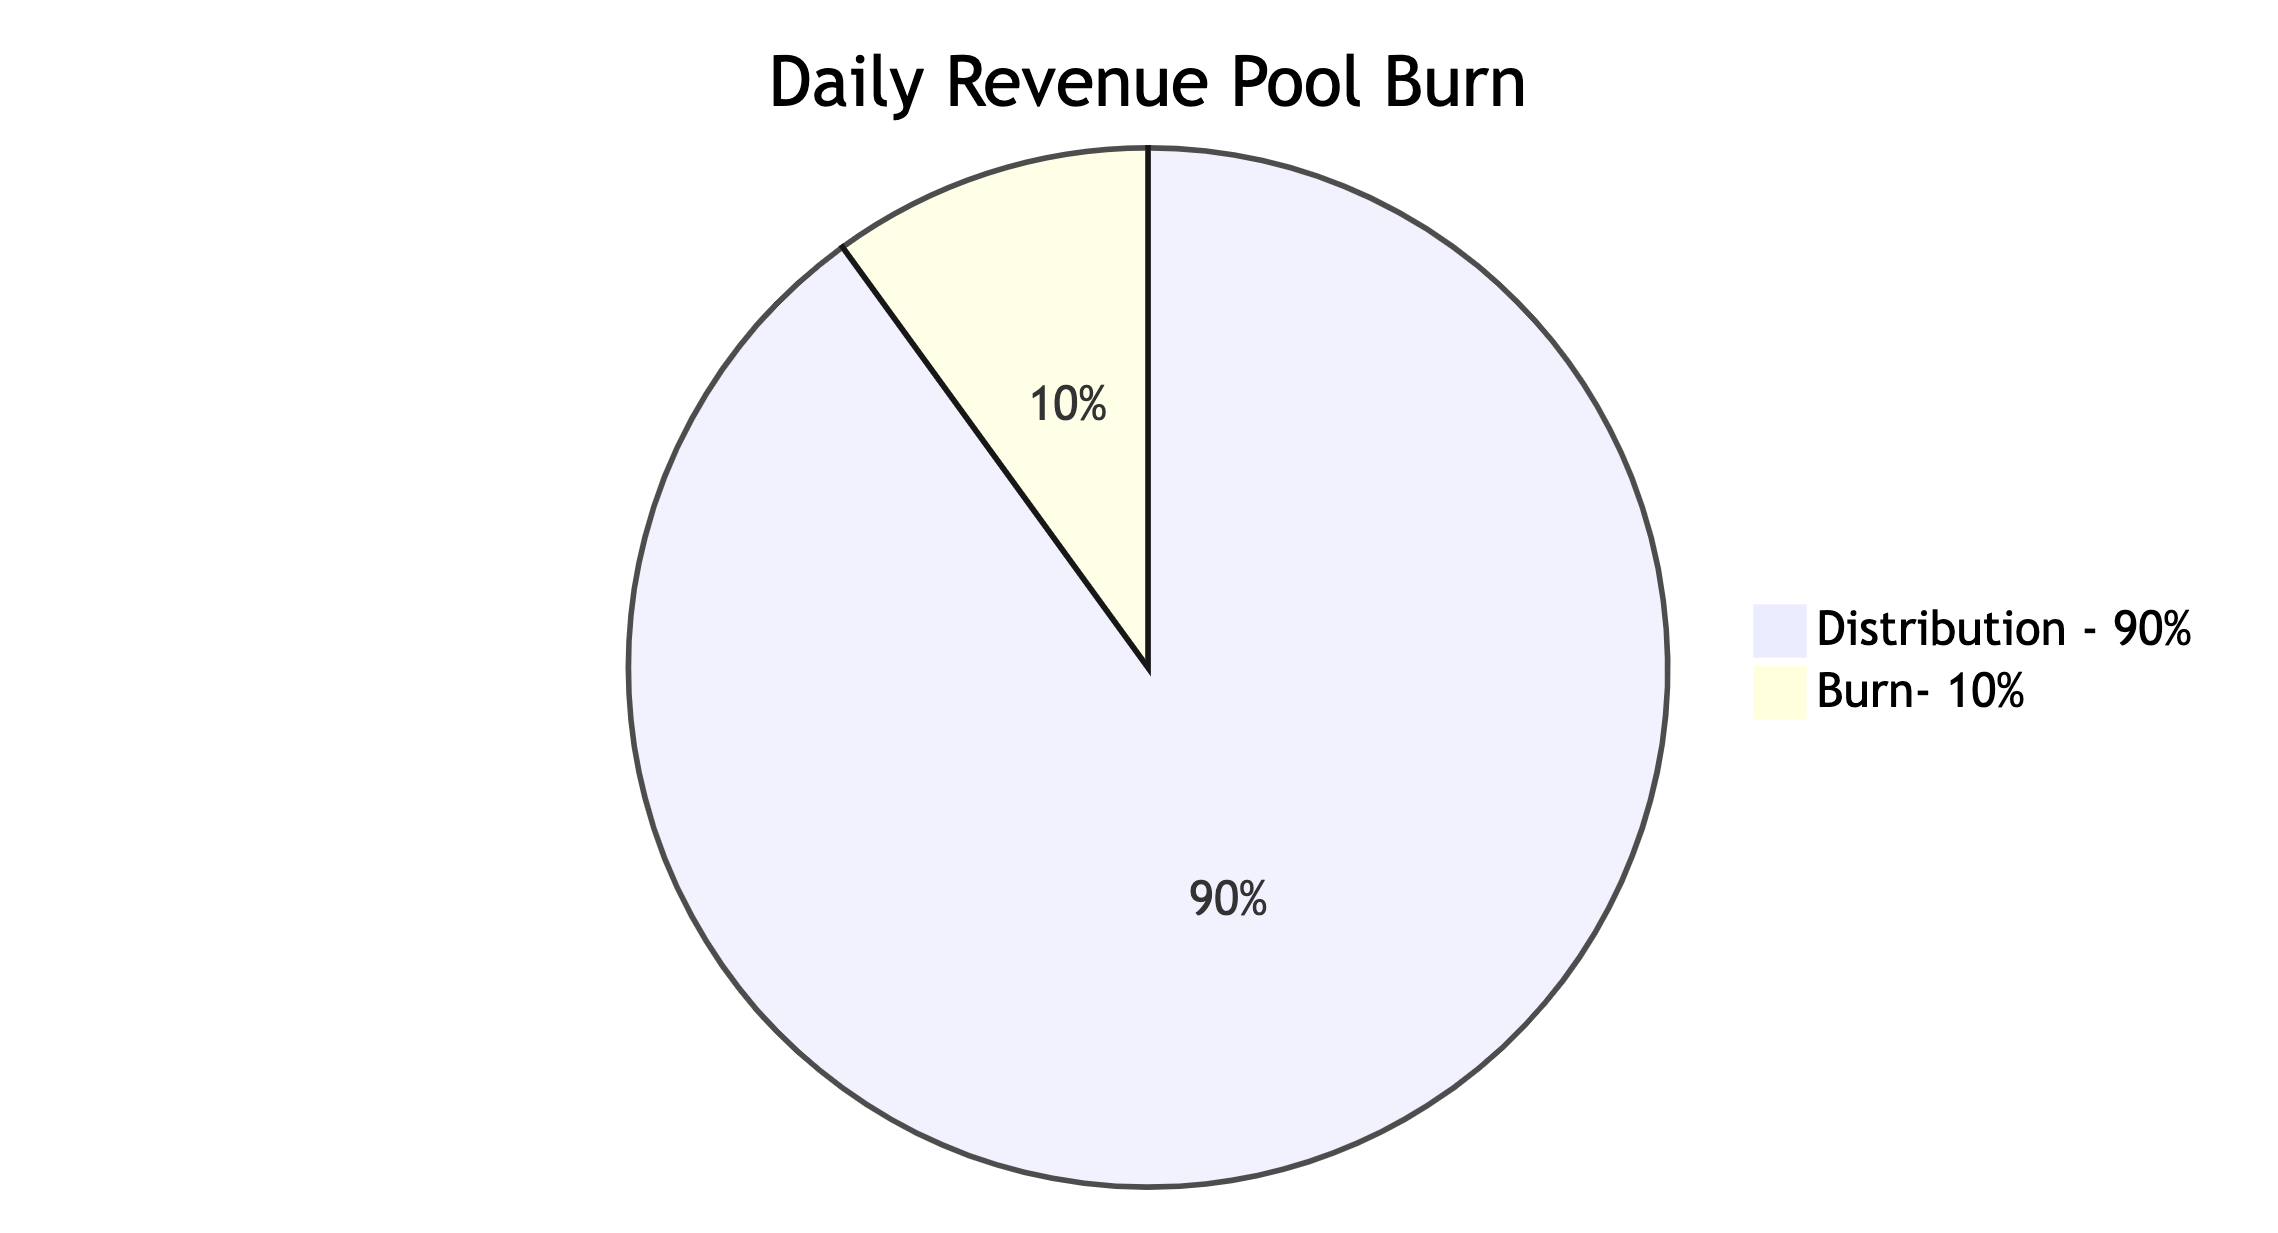
\includegraphics[width=10cm]{burn-chart}
\caption{Burn percentage from Global Reward Pool}
\end{center}
\end{figure}

\begin{figure}[H]
\begin{center}
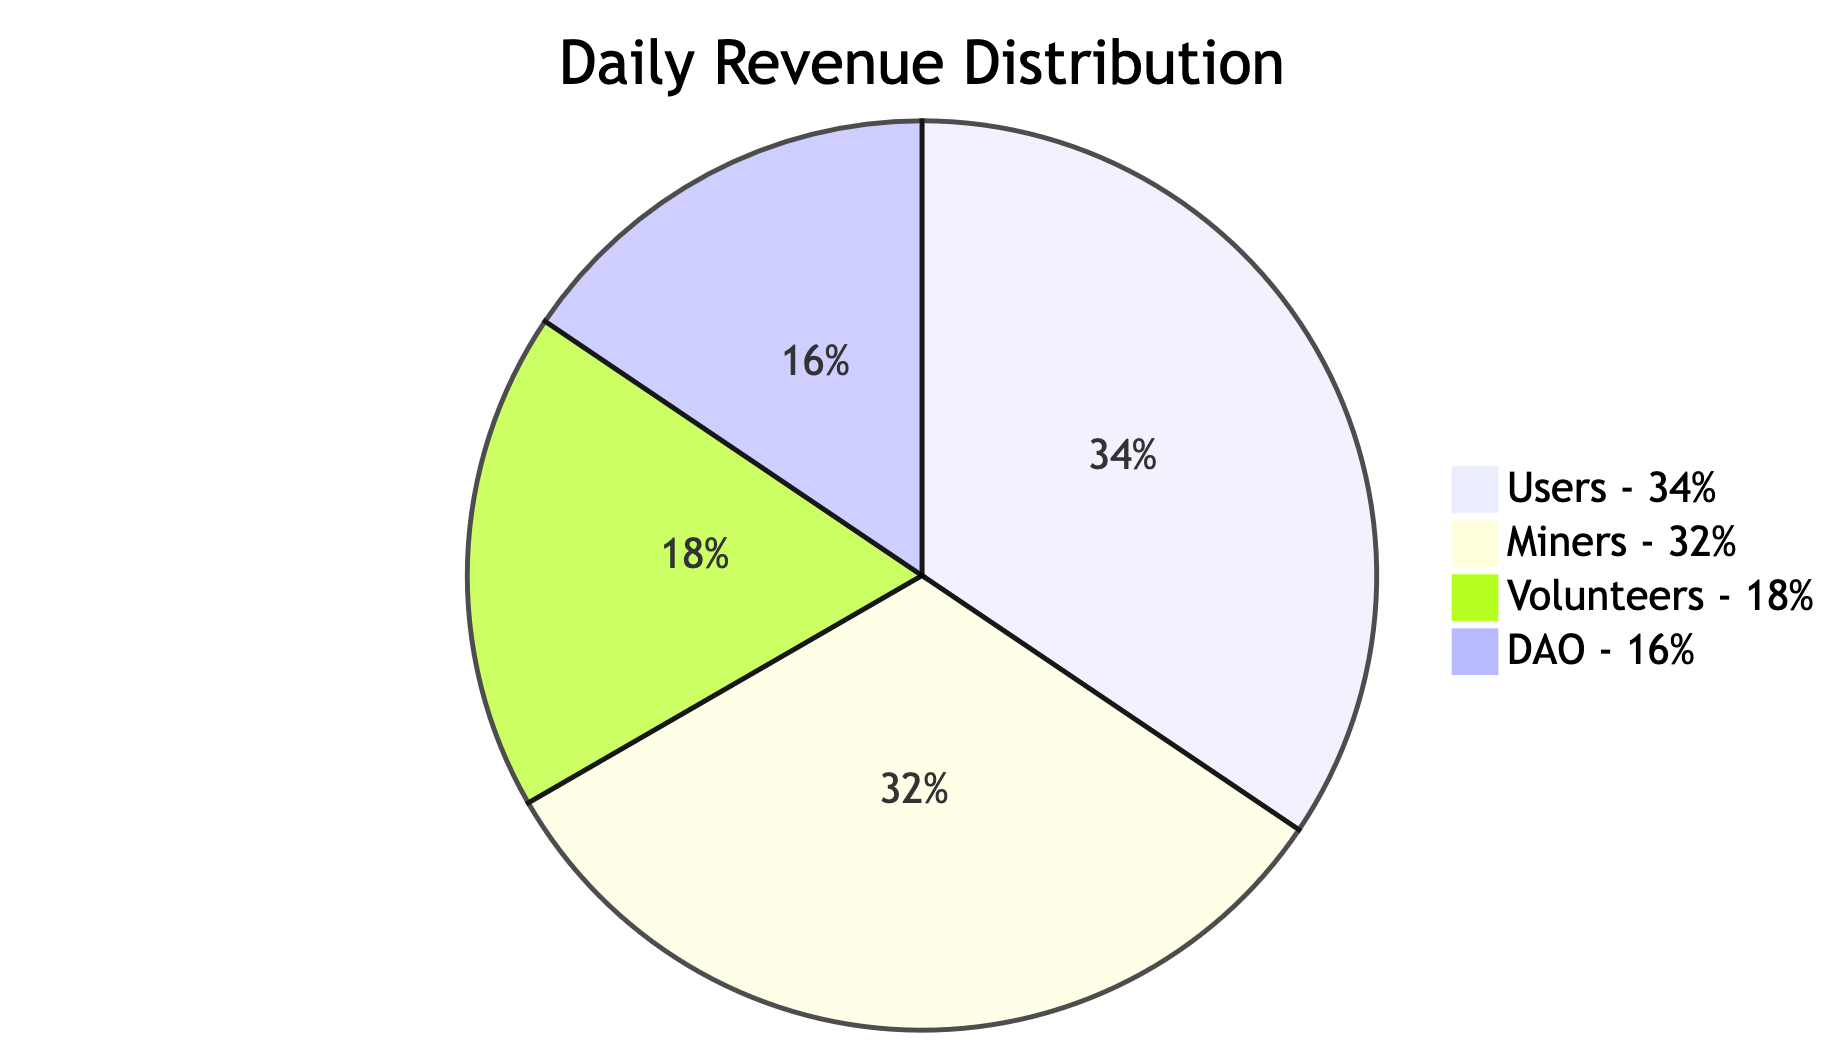
\includegraphics[width=10cm]{revenue-distribution}
\caption{Total Distribution of Funds excluding burn}
\end{center}
\end{figure}


\begin{comment}%mermaid

pie

    title Daily Revenue Distribution
    "Users - 39%" : 35
    "Miners - 31%" : 28
    "Volunteers - 17%" : 15
    "DAO - 13%" :  12


pie

    title Reward Pool
    "Block-chain Miners - 11% " : 11
    "DAG Miners - 5% " : 5
    "Social Miners - 4% " : 4
    "IPFS Miners - 8% " :  8
    "Social Users - 30% " : 30
    "Developers - 6.5% " : 6.5
    "Bounties - 2% " : 2
    "Cryptoback - 5%" : 5
    "Burn - 10% " : 10
    "ROV - 6.5% " : 6.5
    "DAO - 12% " : 12   
   
  
\end{comment}











\subsection{Social Users (Impression-based) - 30\%}

30\% of rewards from the global reward pool is allocated to Application Users based on the total views/impressions users get on their profiles. Impressions counts are agnostic to the type of content that is published in the Viral Application. Impressions/Views are a basic engagement of a typical post in all of social networking platforms. This ensures every content creator on the platform will get rewards according to their reach, popularity, and usage they get for their content on the decentralized platform. This can keep content creators getting paid every day according to the traffic they receive on their profile/content they post.\\

\textbf{Advantages}
\begin{itemize}[leftmargin=+0.2in]
\item Creators can be able to create content expecting a reward for it
\item A fair share of rewards according to the popularity of the content.
\item Users will trust the platform which gives them 30\% of it’s daily collected revenue to every user without any centralized company meddling.
\item Encourages other platform users to join and receive rewards.
\end{itemize}


\textbf{Segregation of Rewards}\\

Global Impressions of all users will be taken to calculate each user’s individual percentage which will be required to allocate individual reward amount from the User Reward Pool.\\

\begin{equation}
User\:Percentage(U_p)=\frac{User\:Total\:Impression(U_i)}{Global\:Impression(G)} \times 100
\end{equation}

\begin{equation}
User\:Rewards(x)=\frac{Total\:Rewards(T) \times User\:Reward\:Percentage(U_p)}{100}
\end{equation}\\

\begin{lstlisting}[language=Solidity, caption={Example User Reward Contract in Solidity}, numbers=none]


// SPDX-License-Identifier: MIT

pragma solidity ^0.8.4;

import "@openzeppelin/contracts@4.5.0/token/ERC20/ERC20.sol";
import "@openzeppelin/contracts@4.5.0/token/ERC20/extensions/ERC20Snapshot.sol";
import "@openzeppelin/contracts@4.5.0/access/Ownable.sol";
import "@openzeppelin/contracts@4.5.0/security/Pausable.sol";

contract Reward is Ownable, Pausable {
   
    uint256 public rewardamount;
    uint256 public rewardfortheuser;
    uint256 public impression = 0.0;
    uint256 public totalimp = 0;


    function pause() public onlyOwner {
        _pause();
    }

    function unpause() public onlyOwner {
        _unpause();
    }
    
    function totalrewardamount() external view onlyOwner returns(uint256){     // read 
         return rewardamount;
    }

    function finalimpression() external view onlyOwner returns(uint256){         //read
        return impression;
    }
    function finalrewardforuser() external view onlyOwner returns(uint256){      //read
        return rewardfortheuser;
    }

    function totalimpressionoftheday(uint256 totalImpressionOfTheDay) public onlyOwner{  //write
          totalimp = totalImpressionOfTheDay;
    }
    
    function claim(uint256 impressionoftheuser) public {                         //claim function
        require(totalimp != 0,"you cant claim your rewards yet");
        require(rewardamount != 0,"you cant claim your rewards yet");
        impression = ((impressionoftheuser*100) / totalimp);
        rewardfortheuser = (rewardamount * impression)/100 ;
        payable(msg.sender).transfer(rewardfortheuser);
    }

}
\end{lstlisting}


\textbf{Example User-Reward}\\

Input:\\
User Impression = 10,000\\
Global Impression = 1,000,000,000\\
Total Reward = 80,000 VRL, 500 BTC, 700 ETH, 1200 SOL \\

\begin{equation}
User\:Percentage(U_p)=\frac{10,000}{1,000,000,000} \times 100 = 0.001\%
\end{equation}
\begin{equation}
User\:Rewards(VRL)=\frac{80,000 \times 0.001}{100} = 0.8\:VRL
\end{equation}
\begin{equation}
User\:Rewards(BTC)=\frac{500 \times 0.001}{100} = 0.005\:BTC
\end{equation}
\begin{equation}
User\:Rewards(ETH)=\frac{700 \times 0.001}{100} = 0.007\:ETH
\end{equation}
\begin{equation}
User\:Rewards(SOL)=\frac{1200 \times 0.001}{100} = 0.012\:SOL
\end{equation}
Output:\\

User Percentage of Rewards : 0.001\%\\
User Reward : \\
0.8 VRL \\
0.005 BTC \\
0.007 ETH \\
0.012 SOL\\


The reward allocation and analysis of coins for each User(Views-Based) will be done at 2.00 AM UTC every day. The users can collect their activity-based rewards manually within a stipulated period of 15 hours. Manual collection of rewards are specifically brought to ensure that the non-active users on the platform will not receive the rewards and only the people who contribute to the platform by being active will be receiving their rewards. The non-active users' coins will be sent to the burn address, where the coins will be sent to burn pool after the stipulated time period finishes. This creates a daily deflationary effect to the Viral Coin that will benefit other wallet users who hold Viral Coins.\\

\subsection{DAO - 12\%}

\subsection{Blockchain-Miners (Gas-based) - 11\%}

\subsection{Burn - 10\%}

\subsection{IPFS-Miners (Storage-based) - 8\%}


\subsection{ROV (Contribution-based) - 6.5\%}

7.5\% of rewards from the global reward pool is allocated to ROV (Republic of Viral), a content moderation community for the Viral Decentralized platform. There, curators will be filtering and voting posts to eliminate spam, inappropriate content which is reported by users and also govern the application's content in a democratic nature considering every curator's vote. This method of democratic voting community eliminates the power of a single individual to decide the type of content if it's violating the social media's posting guidelines. \\

This ensures rapid results in removing explicit content in a relatively short time without any hassles. In short, ROV is a decentralized autonomous organization to maintain Viral's media contents at its best. The curators will be rewarded by Viral Coins for their contribution to the network.\\

\textbf{Advantages of ROV over Centralized Organization}
\begin{itemize}[leftmargin=+0.2in]
\item Faster content removals
\item The decision of a single organization/person will be eliminated
\item A better-decentralized approach to centralized organizations
\item Will work in any time zone 24/7 without any hassles
\end{itemize}

\textbf{Segregation of Rewards}\\

The segregation will be done at 2 AM UTC where the curator's Plus points for the day will be taken and the percentage of rewards will be determined using it. For every vote and every positive contribution they make the points will be increased in the ROV Profile where the curators will get their fair share of rewards considering the total points collected by all curators in 24 hours similar to the segregation algorithm of Users Views-based. Every curator will receive their rewards directly to their wallets where they should collect them manually in a period of 15 hours.\\

\subsection{Social Miners (Serving based) - 4\%}

Social Miners are people running nodes in the viral decentralized network for storing media and data transfers. It is similar to blockchain mining nodes but here the nodes will run Gun DB Relay server, WebRTC signaling server, and other several mini peers of other stacks simultaneously to provide faster data transfer, decentralization of data, higher encryption, better stability, etc. Users can download the node software and run the program to become a social node for the Viral network and start earning rewards according to the data served for the network\\

The segregation will take place at 2 AM UTC by taking the total number of data served from each technology stack's peer such as GUN, WebRTC, and all other mini peers. The points will be given to Social Nodes based on the percentage they served to total served by all stabilizers in the given 24 hours. The stabilizers can able to receive their Daily rewards to their wallets based on contribution, where the rewards have to be collected manually within the 15 hour stipulated window, in which the uncollected coins will be sent to burn address automatically.\\


\subsection{Developers (Contribution-based) - 7.5\%}

7.5\% of rewards from the global reward pool is allocated to Developers. Viral is an Open-source platform where developers contribute to development of the beta application which will be available as an open repository. To give rewards for developers' contribution to the decentralized platform and also to encourage developers by giving paid rewards to structure a better, safer, secure social media for the masses using collaborative work is the ultimate goal. By bringing mass development to life we can ensure that the people who run social media will be the product of hundreds of developers working every day for a common goal of a powerful social communication platform.\\

We will be linking developers' GitHub and viral accounts in a separate ROV-Dev Application in which the developers can contribute their work and get voted by other developers for rewards. The votes will determine their rewards where the maximum voted contribution will receive more viral coins than the minimum voted contribution.\\ 

Developers are the backbone of Viral. Every single developer should be rewarded fairly for their work and the rewards should be determined by their fellow developers inside the community. Since there is no meddling of Viral DAO and its executives, the developer platform will be democratic, decentralized, and autonomous to keep the social media strong and secure in the most possible way. By rewarding developers, we can expect other developers to join the people-run social media.\\

Viral will give a better world to developers expecting a reward for their contribution and also engages a lot of developers into a small community to get most of the percentage from the allocated 7.5\% of daily revenue to a closed community. This will encourage autonomous development of superior technology where all hands matter. \\

The segregation takes place every day at 2 AM UTC according to the votes they got for every single contribution to the beta platform and future plans. Every developer can vote on the done contribution by other developers on a special ROV-Dev Application. This will determine the popularity of the contribution and give fair rewards to each. The rewards will be sent to the Developers' wallets for manual collection which will be available to collect for a period of 15 hours every day.\\

\subsection{DAG-Miners (Transaction-based) - 5\%}

\subsection{Crypto-Back - 5\%}

\subsection{Bounties (DAO-Vote) - 2\%}


\subsection{Charity Contribution}

If the user opts for transferring the rewards to a Non-Profit-Organizations it can be easily transferred directly to the user's preferred Charity. Viral will have a registration portal for Charities to Register their information and get verified to appear on the Application's Wallet.\\ 

\section{Governance \& Viral DAO}

Viral incorporates a vast ecosystem of blockchains and De-Fi application along with the integration of social networking for the masses to adopt cryptocurrencies to the fullest. While aiming for a true-decentralized product, governance plays a huge role in every aspect of decisions on updating the protocols. Most de-fi organizations have separate on-chain governance communities apart from offline-governance to vote and improve their platforms, Viral prepared to seperate governance of current and future products into two governance models and bring decentralized decision making oppurtunity for the members of the community. The Viral Foundatoin decided not to bring in any centralized governance model for any of it's ecosystem except the ViralFEX since it complies with regulatory restrictions.\\

\textbf{Governance Models}\\

\begin{figure}[H]
\begin{center}

\begin{forest}
  forked edges,
  for tree={edge+={-Latex}},
  [Governance
    [Smart Chain Governance
    ]
   [Ecosystem Governance
    ]
  ]
\end{forest}
\caption{Governance Model}
\end{center}
\end{figure}

While governing Viral Smart Chains protocols requires validators and nodes on voting consensus, the mobile application comprising de-fi protocols requires a decentralized autonomous organization (DAO) to vote on frequent updates and maintenance of offline compliances. This model for governance is seperated among validators (miners) and DAO Token Holders.\\


\textbf{Viral Smart Chain}\\

On-Chain Governance\\
Staked Tokens\\
Viral Improvement Proposal\\
Addition of New Chains\\


\textbf{Viral Ecosystem Governance}\\



DAO Intro\\
List of Governing Platforms\\
Viral DAO Tokens\\
Holding Benefits\\
DAO Platform\\
DAO Revenue\\
Distribution and Dividends\\
Viral Operations Cost Structure Proposals\\
DAO Treasury and Decisions\\
Intial DAO Coin Offering\\
DAO Bylaws\\

\section{Tokenomics \& ICO}

\begin{enumerate}[leftmargin=+0.2in]
\item \textbf{Name of the Utility-Token} : Viral Coin
\item \textbf{Ticker of the Token} : VRL
\item \textbf{Pre-mined Tokens} : 5,000,000,000 Tokens will be issued 
\item \textbf{Supply Hard-Cap} : 5,000,000,000 Tokens
\item \textbf{Token Nature} : Deflationary
\end{enumerate}
\begin{figure}[H]
\begin{center}

\includegraphics[width=2.5cm]{viral-coin-logo}
\caption{Viral Coin Logo}
\end{center}
\end{figure}

\begin{figure}[H]
\begin{center}
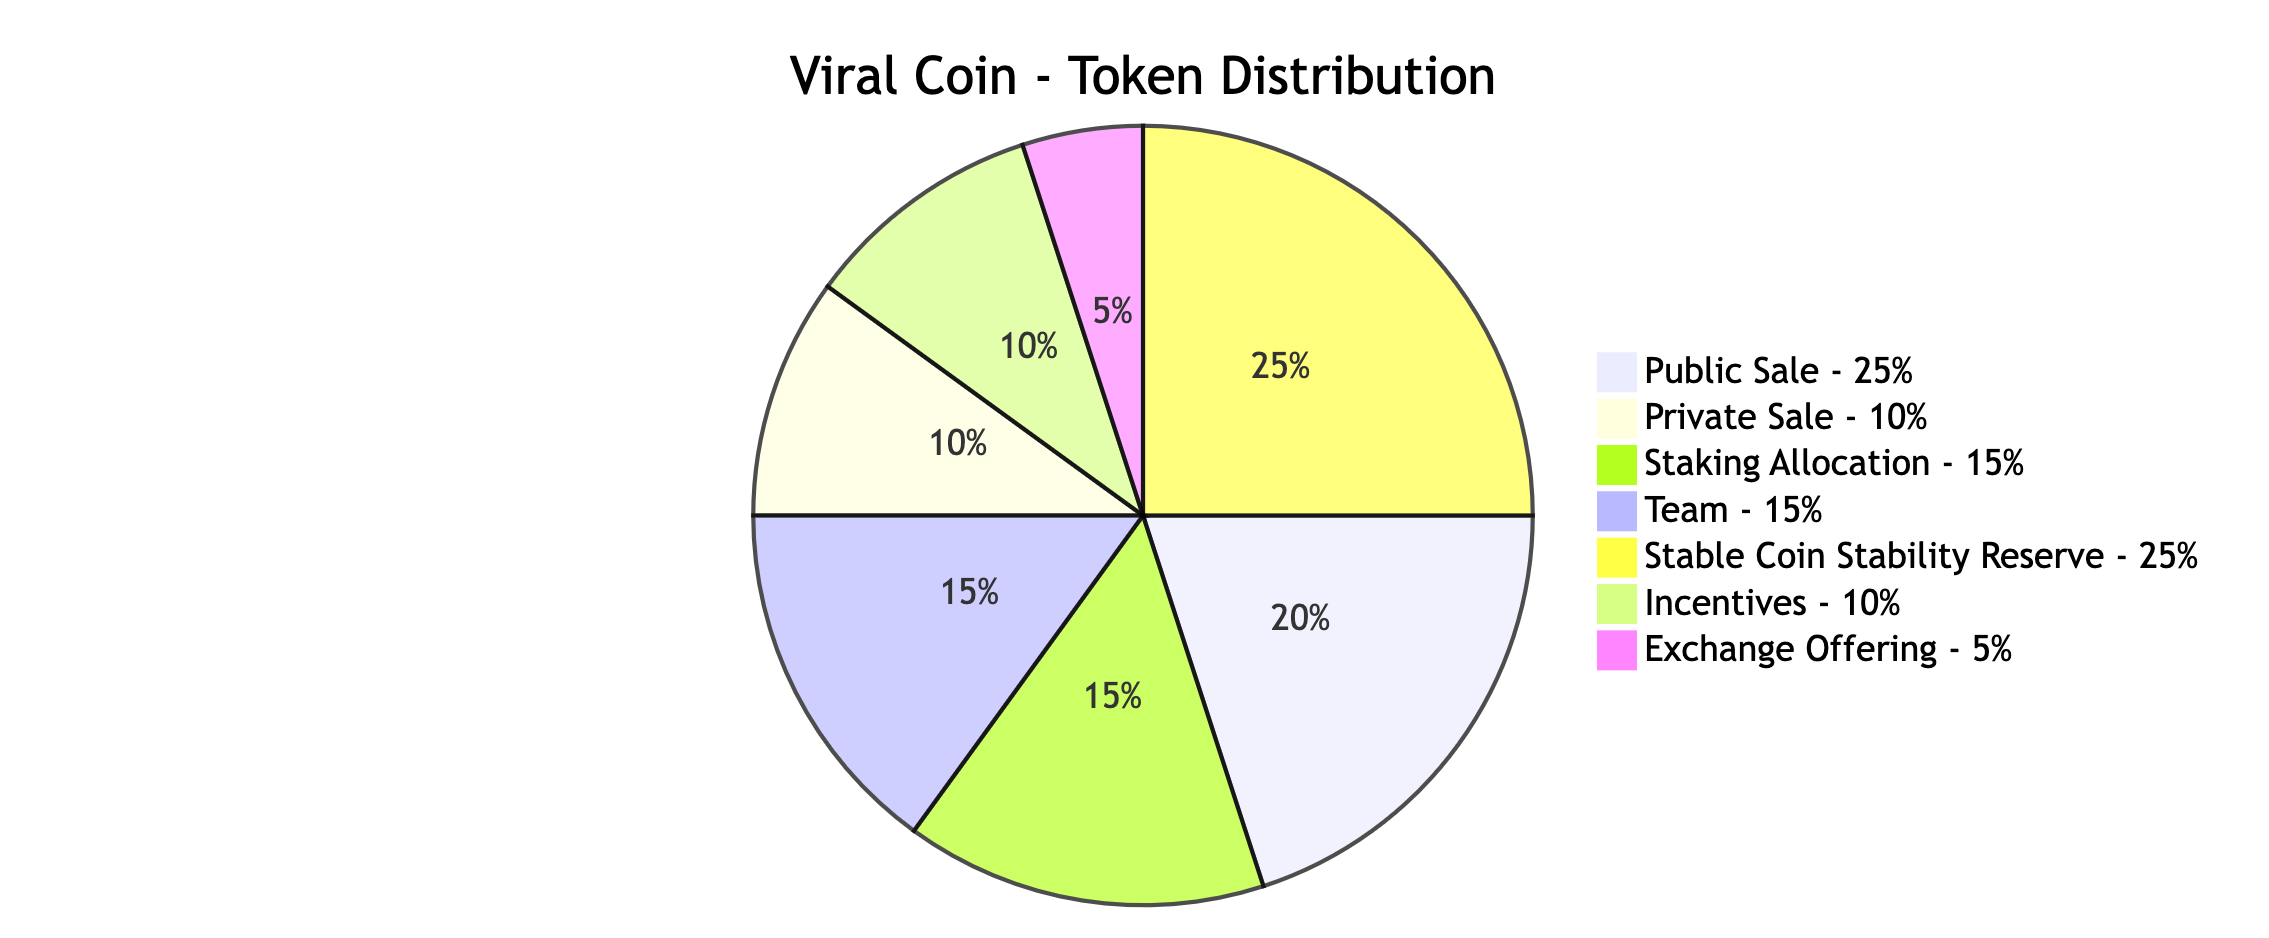
\includegraphics[width=\textwidth]{token-distribution}
\end{center}
\end{figure}


\begin{center}
\begin{table}[!ht]
    \centering
    \begin{tabular}{|l|l|l|l|l|}
    \hline
        \textbf{Sl.no} & \textbf{Round} & \textbf{Supply} & \textbf{Tokens} & \textbf{Price} \\ \hline
        1 & Pre-Seed & Private - 3 \% & 150,000,000 & ~ \\ \hline
        2 & Seed & Private - 4.5 \% & 225,000,000 & ~ \\ \hline
        3 & Pre-Sale & Private - 1.5 \%,  Public (White-list) - 7 \%  & 425,000,000 & ~ \\ \hline
        4 & Main-Sale & Private -  1 \%, Public - 10 \% & 550,000,000 & ~ \\ \hline
        5 & Alpha-Sale & Public - 8 \% & 400,000,000 & ~ \\ \hline
        6 & Exchange Offering & IEO - 5 \% & 250,000,000 & ~ \\ \hline
    \end{tabular}
\end{table}
\end{center}



\begin{comment}
pie

    title Viral Coin - Token Distribution
    "Public Investors - 20%" : 20
    "Private Investors - 10%" : 10
    "Staking Allocation - 15%" : 15
    "Team - 15%" : 15
    "Stable Coin Stability Reserve - 25%" :  25
    "Incentives - 10%" : 10
    "Exchange Offering - 5%" : 5

\end{comment}

\textbf{Intro to Token}\\


\textbf{Deflationary}\\


\textbf{Utility Cases}\\


\textbf{Price Predictions}\\


\subsection{Token Distribution \& Why}


\subsection{Token Sales with Incentives \& Vesting Info}


\subsection{Investor Exit Strategies}




\section{Development Roadmap}

Phase 1 - Beta Launch, Alpha Launch
Phase 2 - External Upgrades\\
Phase 3 - Internal Upgrades\\




\section{Future Plans}

\section{Development}

\begin{table}[!ht]
    \centering
    \begin{tabular}{|c|c|c|c|c|}
    \hline
        Sl.no & Name of the Project & Custom Code & Custom + Fork & Full Fork \\ \hline
        1 & Decentralized Exchange & \checkmark & - & - \\ \hline
        ~ & ~ & ~ & ~ & ~ \\ \hline
        ~ & ~ & ~ & ~ & ~ \\ \hline
        ~ & ~ & ~ & ~ & ~ \\ \hline
        ~ & ~ & ~ & ~ & ~ \\ \hline
        ~ & ~ & ~ & ~ & ~ \\ \hline
        ~ & ~ & ~ & ~ & ~ \\ \hline
    \end{tabular}
\end{table}

\section{ICO Funds Allocation}



\section{Team}

\section{References}

\section{Glossary}











































\end{document}



